\documentclass[11pt, a4paper, titlepage, listof=totoc, bibliography=totoc, index=totoc, twoside, openright, headings=normal]{scrreprt}
\usepackage[ngerman]{babel}
\usepackage[T1]{fontenc}% wichtig für Trennung von Wörtern mit Umlauten
\usepackage{microtype}% verbesserter Randausgleich
\usepackage[utf8]{inputenc}
\usepackage{amsmath}
\usepackage{amsfonts}
\usepackage{amssymb}
\usepackage{graphicx}
\usepackage{fancyhdr}
\usepackage{multirow, tabularx}
\usepackage{setspace}
\usepackage[right]{eurosym}
\usepackage{acronym}
\usepackage{subfig}
\usepackage{floatflt}
\usepackage[usenames,dvipsnames]{color}
\usepackage{colortbl}
\usepackage{paralist}
\usepackage{array}
\usepackage{titlesec}
\usepackage{parskip}
\usepackage[right]{eurosym}
\usepackage{picins}
\usepackage[subfigure,titles]{tocloft}
\usepackage[pdfpagelabels=true]{hyperref}
\usepackage{chngcntr}
\counterwithin{figure}{chapter}
\usepackage{natbib}
\bibliographystyle{dinat}

\usepackage{listings}
\lstset{basicstyle=\footnotesize, captionpos=b, breaklines=true, showstringspaces=false, tabsize=2, frame=lines, numbers=left, numberstyle=\tiny, xleftmargin=2em, framexleftmargin=2em}
\makeatletter
\def\l@lstlisting#1#2{\@dottedtocline{1}{0em}{1em}{\hspace{1,5em} Lst. #1}{#2}}
\makeatother

\usepackage[left=40mm, right=20mm, top=30mm, bottom=30mm]{geometry}

\hypersetup{unicode=false, pdftoolbar=true, pdfmenubar=true, pdffitwindow=false, pdfstartview={FitH},
	pdftitle={Abschlussarbeit},
	pdfauthor={Philipp Anders},
	pdfsubject={Bachelorarbeit},
	pdfcreator={\LaTeX\ with package \flqq hyperref\frqq},
	pdfproducer={pdfTeX \the\pdftexversion.\pdftexrevision},
	pdfkeywords={Bachelorarbeit},
	pdfnewwindow=true,
	colorlinks=true,linkcolor=black,citecolor=black,filecolor=magenta,urlcolor=black}
\pdfinfo{/CreationDate (D:20110620133321)}

\makeatletter
\renewcommand*\l@figure{\@dottedtocline{1}{1.5em}{3em}}
\makeatother
\makeatletter
\def\l@lstlisting#1#2{\@dottedtocline{1}{1.5em}{3em}{#1}{#2}}
\makeatother
\begin{document}

\titlespacing{\section}{0pt}{12pt plus 4pt minus 2pt}{-6pt plus 2pt minus 2pt}

% Kopf- und Fusszeile
\renewcommand{\sectionmark}[1]{\markright{#1}}
\renewcommand{\leftmark}{\rightmark}
\pagestyle{fancy}
\lhead{}
\chead{}
\rhead{\thesection\space\contentsname}
\lfoot{}
\cfoot{}
\rfoot{\thepage}
\renewcommand{\headrulewidth}{0.4pt}
% \renewcommand{\footrulewidth}{0.4pt}

% Vorspann
\renewcommand{\thechapter}{\Roman{chapter}}
\pagenumbering{Roman}
\raggedbottom

% ----------------------------------------------------------------------------------------------------------
% Titelseite
% ----------------------------------------------------------------------------------------------------------
\thispagestyle{empty}
\begin{center}
	\vspace*{1cm}
	\textbf{Hochschule für Technik, Wirtschaft und Kultur Leipzig}\\
	\vspace*{0.3cm}
	Fakultät Informatik, Mathematik und Naturwissenschaften\\
	Bachelorstudiengang Medieninformatik\\
	\vspace*{1cm}
	Bachelorarbeit\\
	zur Erlangung des akademischen Grades\\
	\vspace*{0.3cm}
	\textbf{Bachelor of Science (B.Sc.)}\\
	\Huge
	\vspace*{1cm}
	\textbf{Integration des Tacton Produktkonfigurators in ein Open Source Shopsystem}\\
	
	\vfill
	\normalsize
	\newcolumntype{x}[1]{>{\raggedleft\arraybackslash\hspace{0pt}}p{#1}}
	\begin{tabular}{x{3cm}p{10cm}}
		\rule{0mm}{5ex}\textbf{eingereicht von:} & Philipp Anders\newline Matrikelnummer: 58359 \\ 
		\rule{0mm}{5ex}\textbf{Betreuer:} & Prof. Dr. Michael Frank (HTWK Leipzig)\newline Dipl.-Wirt.-Inf. (FH) Dirk Noack (Lino GmbH)\\ 
		\rule{0mm}{5ex}\textbf{Abgabedatum:} & 28.09.2015 \\ 
	\end{tabular} 
\end{center}
\pagebreak

%% ----------------------------------------------------------------------------------------------------------
% Abstract
% ----------------------------------------------------------------------------------------------------------
\setcounter{page}{1}
\onehalfspacing
\titlespacing{\section}{0pt}{12pt plus 4pt minus 2pt}{2pt plus 2pt minus 2pt}
\section*{Kurzfassung}
Das ganze auf Deutsch.

\vspace{-1,2em}
\titlespacing{\section}{0pt}{12pt plus 4pt minus 2pt}{-6pt plus 2pt minus 2pt}
\section*{Abstract}
Das ganze auf Englisch.
\pagebreak

% ----------------------------------------------------------------------------------------------------------
% Verzeichnisse
% ----------------------------------------------------------------------------------------------------------
% TODO Typ vor Nummer
\renewcommand{\cfttabpresnum}{Tab. }
\renewcommand{\cftfigpresnum}{Abb. }
\settowidth{\cfttabnumwidth}{Abb. 10\quad}
\settowidth{\cftfignumwidth}{Abb. 10\quad}

\rhead{Inhaltsverzeichnis}
\setcounter{secnumdepth}{3} 
\setcounter{tocdepth}{3}
\tableofcontents
\pagebreak
\rhead{Verzeichnisse}
\listoffigures
\pagebreak
\listoftables
\pagebreak
\renewcommand{\lstlistlistingname}{Listing-Verzeichnis}
\lstlistoflistings
\pagebreak

% ----------------------------------------------------------------------------------------------------------
% Abkürzungen
% ----------------------------------------------------------------------------------------------------------
\chapter*{Abkürzungsverzeichnis}
\addcontentsline{toc}{chapter}{Abkürzungsverzeichnis} 
\begin{acronym}[WSDL] % längste Abkürzung steht in eckigen Klammern
	\setlength{\itemsep}{-\parsep} % geringerer Zeilenabstand
	\acro{AJAX}{asynchronous JavaScript and XML}
	\acro{API}{Application Programming Interface}
	\acro{ATO}{Assemble-to-Order}
	\acro{B2B}{Business-to-Business}
	\acro{B2C}{Business-to-Customer}
	\acro{CORS}{Cross-Origin Resource Sharing}
	\acro{CSP}{Constraint Satisfaction Problem}
	\acro{etc.}{et cetera}
	\acro{ETO}{Engineer-to-Order}
	\acro{i.d.R.}{in der Regel}
	\acro{JSON}{JavaScript Object Notation}
	\acro{MC}{Mass Customization}
	\acro{MTO}{Make-to-Order}
	\acro{MVC}{Model View Controller}
	\acro{ORM}{objektrelationale Abbildung}
	\acro{PTO}{Pick-to-Order}
	\acro{RPC}{Remote Procedure Call}
	\acro{SOP}{Same-Origin-Policy}
	\acro{UML}{Unified Modeling Language}
	\acro{URI}{Uniform Resource Identifier}
	\acro{vgl.}{vergleiche}
	\acro{WSDL}{Web Service Description Language}
\end{acronym}
\newpage

% ----------------------------------------------------------------------------------------------------------
% Inhalt
% ----------------------------------------------------------------------------------------------------------
% Abstände Überschrift
\titlespacing{\section}{0pt}{12pt plus 4pt minus 2pt}{0pt plus 2pt minus 2pt}
\titlespacing{\subsection}{0pt}{12pt plus 4pt minus 2pt}{-1pt plus 2pt minus 2pt}
\titlespacing{\subsubsection}{0pt}{12pt plus 4pt minus 2pt}{-1pt plus 2pt minus 2pt}

% Kopfzeile
\renewcommand{\sectionmark}[1]{\markright{#1}}
\renewcommand{\subsectionmark}[1]{}
\renewcommand{\subsubsectionmark}[1]{}
\lhead{Kapitel \thesection}
\rhead{\rightmark}

\onehalfspacing
\renewcommand{\thesection}{\arabic{section}}
\renewcommand{\theHsection}{\arabic{section}}
\setcounter{section}{0}
\pagenumbering{arabic}
\setcounter{page}{1}

\chapter{Einleitung}
\begin{quote}
\glqq I'd like a plain omelette, no potatoes, tomatoes instead, a cup of coffee and toast.\grqq{}
\begin{addmargin}[25pt]{0pt} 
\glqq No substitutions.\grqq{}
\end{addmargin}
\glqq What do you mean, you don't have any tomatoes?\grqq{}
\begin{addmargin}[25pt]{0pt} 
\glqq Only what's on the menu. You can have a number 2 -- a plain omelette. It comes with cottage fries and rolls.\grqq{}
\end{addmargin}
\glqq I know what it comes with but it's not what I want.\grqq{}
\end{quote}
Diese Unterhaltung stammt aus der \glqq Diner Scene\grqq{} des Films \glqq Five Easy Pieces\grqq{} (1970). Darin versucht Schauspieler Jack Nicholson verzweifelt, sich ein individuelles Essen aus den Zutaten der Gerichte in der Karte zusammenzustellen. Die Szene endet mit der Explosion des angestauten Frusts über diese umständliche Bestellung, indem er das gesamte Geschirr mit dem Arm vom Tisch fegt.

Diese Situation illustriert auf humorvolle Weise das Problemfeld der Produktkonfiguration. In diesem möchte sich der Kunde ein individuelles Produkt zusammenstellen, da keiner der Standardartikel seinen Vorstellungen entspricht. Die Produktkonfiguration unterstützt den Kunden bei seinen Individualisierungswünschen im Rahmen dessen, was vom Hersteller umsetzbar ist.

Die Produktkonfiguration findet Anwendung in einem breiten Aufgabenfeld. Das kann die einfache Optionsauswahl beim Designen eines individuellen Nike-Schuhs via \emph{NIKEiD} sein oder die Konfiguration eines Flugzeugs durch Fachpersonal mit technischer Expertise. Im Gegensatz dazu steht ein Onlineshop wie z.B. Zalando üblicherweise für den Vertrieb von Standardprodukten. Mit der Auswahl der richtigen Kleidergröße oder -farbe bieten diese Systeme einen eher begrenzten Entscheidungsspielraum.

Die vorliegende Arbeit entstand im Rahmen der Tätigkeit bei der Lino GmbH. Diese vertreibt unter anderem als autorisierter Reseller Produkte der Tacton Systems AB (Tacton), welche eine softwaretechnische Lösung für die Produktkonfiguration in Form des Tacton Produktkonfigurators anbietet. Die Lino GmbH hat den Bedarf von Industrieunternehmen, deren Produktkatalog aus konfigurierbaren Artikeln besteht, zur Erschließung eines direkten Absatzweges via Onlineshop erkannt. Die Integration des Tacton Produktkonfigurators in ein Shopsystem erweitert dessen technische Mittel, um diesem Bedarf gerecht zu werden.

\section{Ziel der Arbeit}
Das Ziel der Arbeit ist die Entwicklung einer softwaretechnischen Lösung, die es dem Anwender ermöglicht, ein Produkt in einem Open-Source Shopsystem zu konfigurieren und zu bestellen, wobei die Konfiguration durch den Tacton Produktkonfigurator realisiert wird. Dabei müssen zwei Systeme betrachet werden -- das Shopsystem und das Konfigurationssystem. Um letzteres in einer neuen Systemumgebung verfügbar zu machen, muss ein entsprechendes Integrationskonzept entworfen werden. Dabei wird geklärt, welche Daten auf welchem Wege auszutauschen sind. Wie weiterhin der konfigurierte Artikel in den Bestellprozess integriert wird, ist abhängig von der konkreten Wahl des Shopsystems. Letztendlich werden ein Plugin für das Konfigurationssystem und ein Plugin für das Shopsystem entwickelt, welche durch deren Zusammenarbeit das Integrationsszenario bewältigen.

\section{Aufbau der Arbeit}
Im Grundlagenteil (Kapitel 2) wird zunächst ein Bezugsrahmen für das Thema Produktkonfiguration geschaffen. Dabei wird geklärt, welche ökonomischen Rahmenbedingungen deren Einsatz motivieren und auf welche Produkte sie anwendbar ist. Das weitere theoretische Fundament leitet sich aus dem Titel der Arbeit \glqq \textbf{Integration} des Tacton \textbf{Produktkonfigurators} in ein Open-Source \textbf{Shopsystem}\grqq{} ab. Zunächst wird die Produktkonfiguration sowie die Softwaresysteme, die diese realisieren, behandelt. Unter der Voraussetzung, dass sowohl das Shopsystem als auch das Konfigurationssystem webfähig sind, werden danach Webservices als Integrationsinstrument erläutert. Abschließend werden Online-Shops in einen ökonomischen Rahmen eingeordnet und typisiert. 

Im Analyseteil (Kapitel 3) werden die konkreten Systeme betrachtet. Dabei wird zunächst der Tacton Produktkonfigurator besprochen. Aus dessen Analyse werden Anforderungen an das Shopsystem abgeleitet. Die Evaluierung der möglichen Kandidaten ist nicht Bestandteil der Arbeit. Es wird ein Shopsystem festgelegt und einer Detailbetrachtung unterzogen. Aus dem Kapitel resultieren die Erweiterungsmöglichkeiten und grundlegenden Verantwortungsbereiche der Systeme im Integrationsszenario.

Aufbauend auf der Analyse werden in Kapitel 4 die funktionalen und nichtfunktionalen Anforderungen für die Integration formuliert. Diese dienen als Orientierungspunkte für die folgende Entwicklung eines Integrationskonzepts in Kapitel 5. Kapitel 6 skizziert die Herangehensweise und den Ablauf der Implementierung.

In Kapitel 7 wird die Lösung diskutiert, wobei Potentiale für zukünftige Entwicklungsarbeiten aufgezeigt werden. Abschließen erfolgt eine anwendungsbezogene Einordnung des Resultats in den ökonomischen Kontext, der im Grundlagenteil umrissen wurde.

\chapter{Grundlagen}
\label{Grundlagen}
\section{Bezugsrahmen}
Im Folgenden wird ein Bezugsrahmen für Produktkonfigurationssysteme (Konfiguratoren) geschaffen. Dazu wird zunächst die marktwirtschaftliche Situation erläutert, welche die Notwendigkeit \emph{hybrider Wettbewerbsstrategien} begründet. Diese wiederum stellen zu ihrer Umsetzbarkeit Bedingungen an \emph{Produktionskonzepte}, welche daraufhin vorgestellt werden.

\subsection{Hybride Wettbewerbsstrategien}
\label{oekonomischerBezug}
Neue Wettbewerbsbedingungen und gesteigerte Kundenansprüche haben den Druck auf Industrieunternehmen zur Produktion individualisierter Produkte erhöht \citep{piller98}. Das entspricht einer stärkeren Forcierung der \emph{Leistungsdifferenzierung} \citep{lutz11}. Diese ist eine der von \citet{porter02} beschriebenen \glqq generischen Wettbewerbsstrategien\grqq{}. Bei der Leistungsdifferenzierung werden Produkte mit höherem individuellen Kundennutzen zu höheren Preisen verkauft. Eine der anderen Wettbewerbsstrategien ist die \emph{Kostenführerschaft}. Diese bezieht sich klassischerweise auf Anbieter von Massenproduktion. Dabei werden die Marktanteile durch die Unterbietung der Konkurrenzpreise gesteigert.

\vspace{1em}
\begin{minipage}{\linewidth}
	\centering
	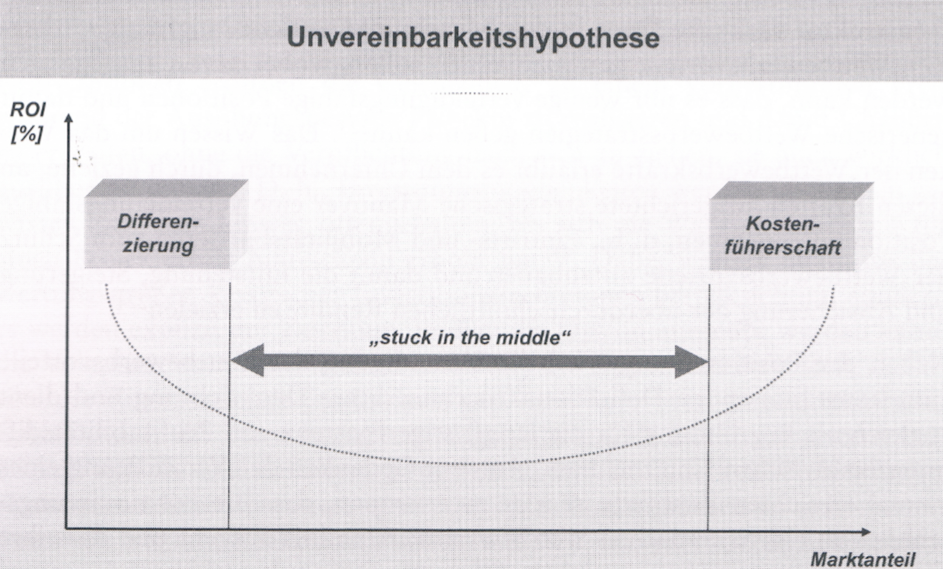
\includegraphics[width=0.7\linewidth]{Abbildungen/unvereinbarkeitshypothese.png}
	\captionof{figure}[Unvereinbarkeitshypothese nach Porter]{Unvereinbarkeitshypothese nach \cite{porter80}, zitiert von \cite{schuh05}}
	\label{fig:unvereinbarkeitshypothese}
\end{minipage}
\vspace{0.3em}

In diesem Zusammenhang formulierte \citeauthor{porter80} die \emph{Unvereinbarkeitshypothese}. So sollen Kostenführerschaft und Leistungsdifferenzierung nicht gleichzeitig erreichbar sein. Eine uneindeutige Positionierung führe zu einem \glqq stuck in the middle\grqq{} und damit zur Unwirtschaftlichkeit, wie Abbildung \ref{fig:unvereinbarkeitshypothese} darstellt.

Die Beobachtung der Unternehmensrealität zeichnet ein anderes Bild. Neue Organisationsprinzipien, Informationsverarbeitungspotentiale und Produktstrukturierungsansätze ermöglichen einen Kompromiss aus Preis- und Leistungsführerschaft \citep{schuh05}. Das Ergebnis wird als \emph{hybride Wettbewerbsstrategien} bezeichnet. Eine dieser Strategien ist die sogenannte \emph{\ac{MC}}.

\ac{MC} ist die \glqq Produktion von Gütern und Leistungen für einen (relativ) großen Absatzmarkt, welche die unterschiedlichen Bedürfnisse jedes einzelnen Nachfragers dieser Produkte treffen, zu Kosten, die ungefähr denen einer massenhaften Fertigung vergleichbarer Standardgüter entsprechen\grqq{} \citep{piller98}. Mit anderen Worten: Preisvorteil (\ac{i.d.R.} durch Massenfertigung) wird mit Individualisierung (\ac{i.d.R.} durch Variantenvielfalt) vereint.

Ein Beispiel für einen Anwendungsbereich von \ac{MC} ist die Automobilindustrie. Hersteller bieten Modelle in verschiedenen Ausführungen an, die der Kunde beim Online-Bestellprozess weiter individualisieren kann (siehe z.B. Opel\footnote{http://www.opel.de/tools/konfigurator/personenwagen.html} und BMW\footnote{http://bmw.de/BMW\_Konfigurator}).

\subsection{Produktklassifizierung}
\label{Produktklassifizierung}

\ac{MC} stellt zu deren Umsetzbarkeit gewisse Bedingungen an die Produktionsweisen der abzusetzenden Güter. Im Folgenden wird eine Klassifizierung von Produkten in Bezug zu deren Herstellung vorgestellt. Die Typen werden als \emph{Produktionskonzepte} bezeichnet (nach \citealt{schuh06}, zitiert von \citealt{lutz11}):
\begin{compactitem}
	\item[\textbf{\ac{PTO}:}] Herstellung ohne Kundenauftrag; Lagerhaltung auf Ebene ganzer Produkte; Keine Abhängigkeit dieser Produkte untereinander;\vspace{0.3em}
	
	Beispiel: Ein Standardnotebook.
	\item[\textbf{\ac{ATO}:}] Herstellung ohne Kundeauftrag; Lagerhaltung auf Ebene der Baugruppen/-teilen; Teile mit Abhängigkeiten untereinander;\vspace{0.3em}
	
	Beispiel: Ein Notebook, bei welchem auf Kundenwunsch statt des CD-Laufwerks eine zusätzliche Festplatte eingebaut wird. Die Festplatte wurde bereits im Lager vorgehalten.
	\item[\textbf{\ac{MTO}:}] Herstellung teilweise erst nach Kundenenauftrag; Lagerhaltung auf Ebene der Baugruppen/-teilen; Produktion oder parametrisierte Konstruktion (d.h. durch Regeln generierte Konstruktionsdaten) von Komponenten nach Kundenanforderung; Abhängigkeiten zwischen Teilen; keine unendliche Anzahl von Varianten;\vspace{0.3em}

Beispiel: Ein Notebook, bei dem der Kunde die Displaygröße abweichend von den Standarddiagonallängen bestimmen kann. Display und Notebookgehäuse müssen konstruiert/hergestellt und die technischen Standardkomponenten (z.B. Festplatte, Motherboard) eingepasst werden. 
	\item[\textbf{\ac{ETO}:}] Produkt ist nicht komplett vom Hersteller vorhersehbar; Wenig bis keine Lagerhaltung auf Ebene der Baugruppen/-teilen; Entwicklung und Fertigung von Teilen nach Kundenspezifikation; unendliche Variantenanzahl möglich;\vspace{0.3em}

Beispiel: Herstellung eines Notebooks mit ausklappbarem Gamepad.
\end{compactitem}

Die Produktionskonzepte unterscheiden sich hauptsächlich danach, wann die Produktion der Baugruppen/-teile beginnt -- vor oder nach Auftragsspezifikation. Eine Produktion vor Auftragseingang, also ohne Kundenspezifikation, erlaubt Lagerhaltung. Ein hoher Komponentenanteil, der erst nach Auftragseingang hergestellt werden kann oder sogar konstruiert werden muss, spricht für eine starke Kundenindividualisierung \citep{lutz11}. Die unterschiedlichen Produktionskonzepte haben jeweils einen Anwendungsbezug zu Konfiguratoren, welche im Folgenden vorgestellt werden.

\section{Produktkonfiguration}
\label{Produktkonfiguration}
 
Aus der \ac{MC} (siehe Kapitel \ref{oekonomischerBezug}) resultiert mehr Produktvariabilität und damit Produktkomplexität. Die \emph{Produktkonfiguration} (Konfiguration) ist ein Werkzeug zur Beherrschung dieser Komplexität. Sie unterstützt das Finden einer Produktvariante, die auf Kundenanforderungen angepasst und gleichzeitig machbar ist \citep{lutz11}.

\subsection{Begriffsüberblick}
\label{begriffsuberblick}
Die \textbf{Konfiguration} ist eine spezielle Designaktivität, bei der der zu konfigurierende Gegenstand aus Instanzen einer festen Menge wohldefinierter Komponententypen zusammengesetzt wird, welche entsprechend einer Menge von Konfigurationsregeln (Constraints) kombiniert werden können \citep{sabin98}.

Die Einordnung als Designaktivität erlaubt außerdem die Beschreibung der Konfiguration als ein Designtyp. Es werden das \emph{Routine Design}, \emph{Innovative Design} und \emph{Creative Design} unterschieden. Die Konfiguration entspricht dem Routine Design. Dabei handelt es sich um ein Problem, bei der die Spezifikation der Objekte, deren Eigenschaften sowie kompositionelle Struktur vorgegeben ist und die Lösung auf Basis einer bekannten Strategie gefunden wird \citep{brown89}. Damit ist Routine Design die simpelste der drei Formen. Die anderen Designtypen enthalten hingegen Objekte und Objektbeziehungen, die erst während des Designprozesses entwickelt werden.

Die Schlüsselbegriffe der Definition von \citeauthor{sabin98} sind Komponententypen und Constraints. \textbf{Komponententypen} sind Kombinationselemente, welche durch Attribute charakterisiert werden und eine Menge alternativer (konkreter) Instanzen repräsentieren. Übertragen auf die objektorientierte Programmierung verhalten sich Komponententypen zu Instanzen wie Klassen zu Objekten. Komponententypen stehen zueinander in Beziehung. Diese kann entweder eine \glqq Teil-Ganzes\grqq{}-Beziehung oder Generalisierung sein \citep{felferning14}. \textbf{Constraints} (d.h. Konfigurationsregeln) im engeren Sinne sind Kombinationseinschränkungen \citep{felferning14}. Auf die eben genannten Begriffe wird in Kapitel \ref{wissenrepraesentation} genauer eingegangen.

Zur besseren Nachvollziehbarkeit der weiteren Terminologie ist eine Definition des Variantenbegriffs angebracht. DIN 199 beschreibt Varianten als \glqq Gegenstände ähnlicher Form und/oder Funktion mit einem in der Regel hohen Anteil identischer Gruppen oder Teile\grqq{}. Varianten sind also Gegenstandsmengen. Ein Element dieser Menge unterscheidet sich von einer anderen durch mindestens eine Beziehung oder ein Element \citep{lutz11}.

Die Einheit aus Komponententypen und dem Wissen um deren Kombinierbarkeit in Form von Constraints wird als \textbf{Konfigurationsmodell} bezeichnet. Es definiert implizit alle Varianten eines Produkts \citep{soininen98}. Dadurch muss nicht jede Variante explizit definiert und abgespeichert werden (z.B. in einer Datenbank). Die Anzahl möglicher Kombinationen kann in die Millionen gehen. Das würde die Suche nach einer bestimmten Variante, die einer vorgegebenen Optionskombination entspricht, sehr zeitaufwändig machen \citep{falkner11}.

Die Einheit aus Konfigurationsmodell und Kundenanforderungen (d.h. den Vorstellungen und Wünschen des Kunden über das Produkt) wird als \textbf{Konfigurationsaufgabe} bezeichnet \citep{felferning14}. Auf deren Grundlage kann die gewünschte Konfiguration errechnet werden. Demzufolge ist der Begriff Konfiguration inhaltlich überladen -- er bezeichnet sowohl den technischen Verarbeitungsprozess der Lösungsfindung als auch die Lösung selbst. Im Folgenden werden daher die Begriffe \textbf{Konfigurationsprozess} sowie \textbf{Konfigurationslösung} verwendet. Der Konfigurationsprozess wird von einem System durchgeführt. Dieses wird als \textbf{Konfigurator} bezeichnet.

Die vorausgehende Beschreibung einer Konfigurationslösung suggeriert, dass zu Beginn des Konfigurationsprozesses einmalig die Konfigurationsaufgabe formuliert und daraufhin die Konfigurationslösung ermittelt wird. Diese Form wird als \textbf{statische Konfiguration} bezeichnet. Demgegenüber erlaubt die \textbf{interaktive Konfiguration} das schrittweise Treffen und Revidieren von Entscheidungen \citep{hadzic04}. Die Menge aller bisher getroffenen Entscheidungen wird als \textbf{Konfigurationszustand} bezeichnet \citep{tactonTCsiteDevelopmentManual}. Ein interaktiver Konfigurator muss beim Konfigurationsprozess einen Mechanismus besitzen, der die Konfigurationsaufgabe in Bezug mit dem Konfigurationszustand bringt.

\subsection{Wissensrepräsentation}
\label{wissenrepraesentation}
Das Wissen, welches über ein konfigurierbares Produkt besteht, wird als  \emph{Konfigurationswissen} bezeichnet \citep{soininen98}. Dieses Wissen kann auf unterschiedliche Art und Weise repräsentiert (d.h. dargestellt) werden. Die Repräsentation kann zur Definition eines Konfigurationsmodells genutzt werden \citep{felferning14}. Auf konzeptioneller Ebene werden die Begriffe Wissensrepräsentation und Konfigurationsmodell äquivalent verwendet. Auf technischer Ebene bezeichnet das Konfigurationsmodell jedoch das spezifische Format, welches ein Konfigurator versteht \citep{soininen98}.

Im Folgenden wird eine grafische Form der Wissensrepräsentation vorgestellt, die auf UML basiert. Die grafische Darstellung wurde gewählt, da durch diese eine Vorstellung über die Problemdomäne gebildet werden kann. Sie ist UML-basiert, da die Sprache in der Informatik zur Wissensmodellierung bekannt ist. Zur Erklärung wird eine Notebook-Konfiguration eingeführt, die im weiteren Verlauf der Arbeit immer wieder aufgegriffen wird. Die Modellierung basiert auf dem Arbeitsbeispiel von \citep{felferning14}. Einzelne Komponenten des Beispiels wirken aus aktueller Sicht überholt, sind zur Veranschaulichung bestimmter Constraints aber bewusst gewählt.

\vspace{1em}
\begin{minipage}{\linewidth}
	\centering
	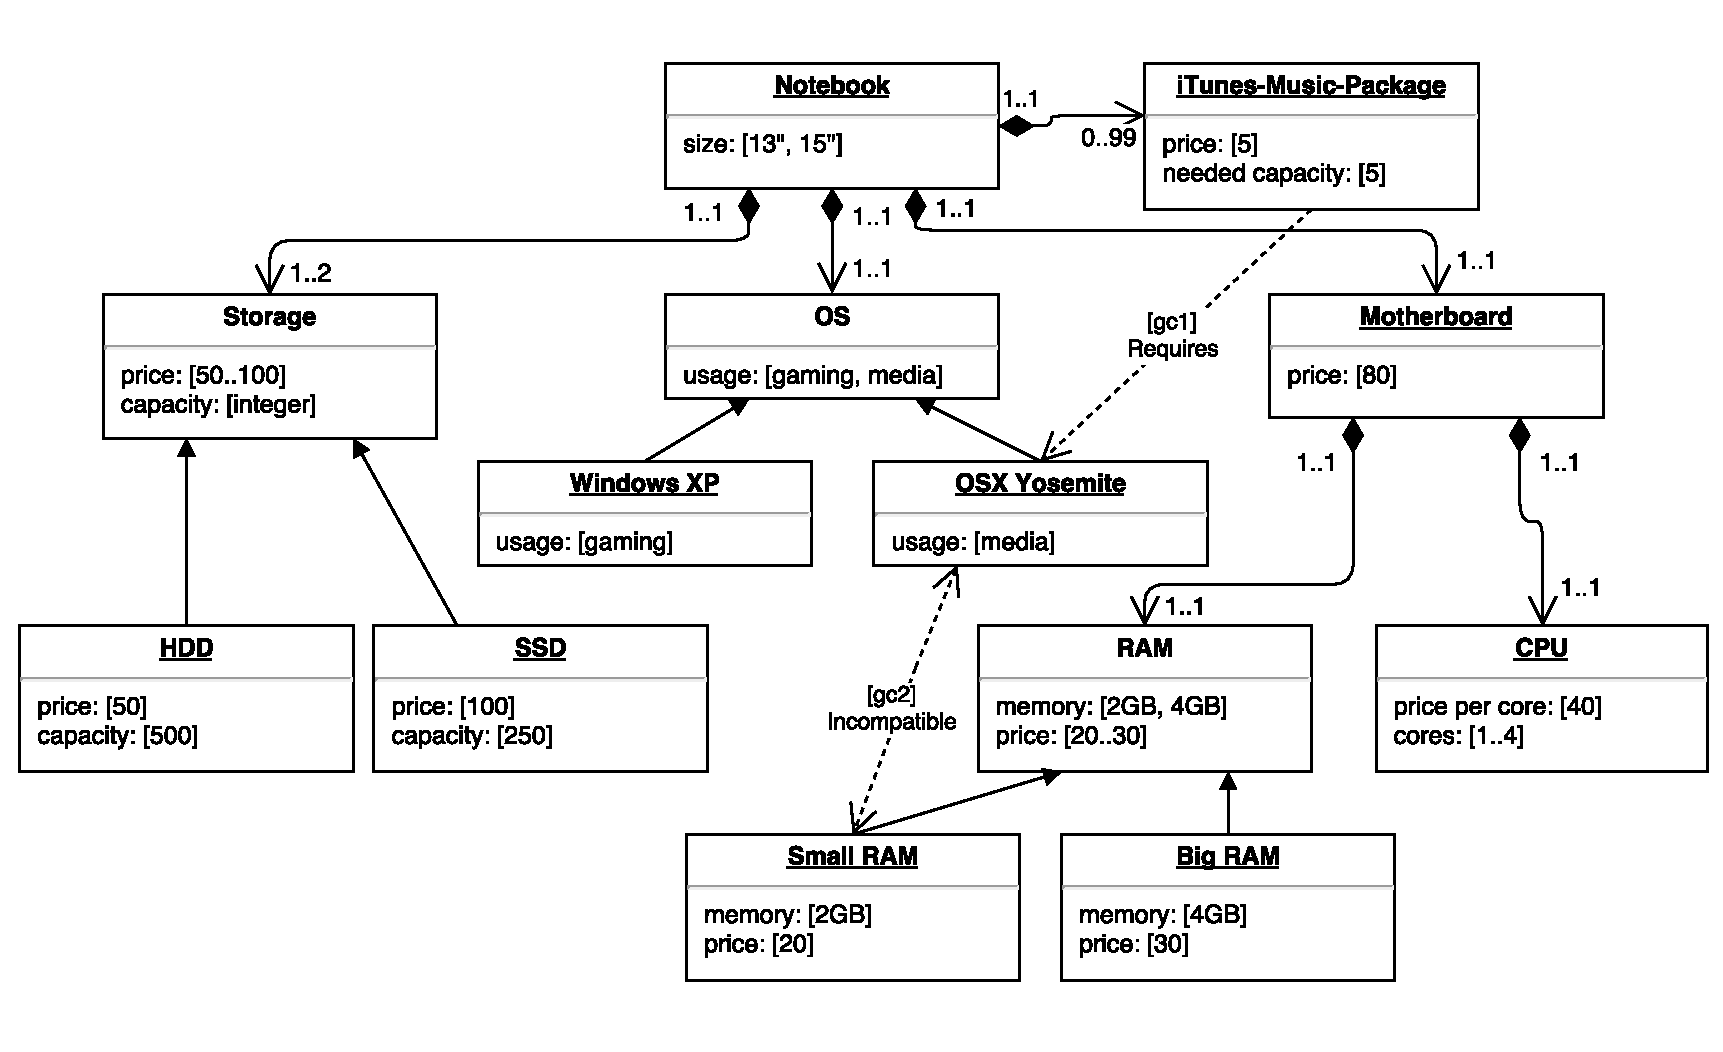
\includegraphics[width=1\linewidth]{Abbildungen/notebookConfigurationUML.pdf}
	\captionof{figure}[UML-Visualisierung der exemplarischen Notebook-Konfiguration]{UML-Visualisierung der exemplarischen Notebook-Konfiguration\footnote{Das 'iTunes-Music-Package' stellt ein Überraschungspaket mit Musik für iTunes dar.}}
	\label{fig:notebookConfigurationUML}
\end{minipage}
\vspace{1em}

\begin{table}[]
\centering
\caption{Constraints des Konfigurationsmodells aus Abbildung \ref{fig:notebookConfigurationUML}}
\label{tab:notebookConfigurationConstraints}
\begin{tabularx}{\textwidth}{|l|X|}
\hline
{\bf Name} & {\bf Beschreibung}\\
\hline
$GC_1$ & Wird das 'iTunes-Music-Package' gewählt, muss auch das Betriebssystem ('OS') vom Typ 'OSX Yosemite' gewählt werden. \\
\hline
$GC_2$ & Das 'OS' vom Typ 'OSX Yosemite' und der Arbeitsspeicher ('RAM') vom Typ ‘Small RAM' können nicht gleichzeitig gewählt werden.\\
\hline
$PRC_1$ & Der Preis des Notebooks ist die Summe der 'price'-Attribute der 'Storage'-, 'Motherboard'-, 'RAM'-, 'CPU'- und 'iTunes-Music-Package'-Instanzen.\\
\hline
$RESC_1$ & Die Summe der 'needed capacity'-Attribute aller 'iTunes-Music-Package'-Instanzen darf die Summe der 'capacity'-Attribute aller 'Storage'-Instanzen nicht überschreiten.\\
\hline
$CRC_1$ & Das 'OS' vom Typ 'OSX Yosemite' benötigt mindestens einen 'core'-Wert der 'CPU' von 2.\\
\hline
$COMPC_1$ & Das OS vom Typ 'Windows XP' ist inkompatibel mit einem 'size'-Wert des Notebooks von 13".\\
\hline
\end{tabularx}
\end{table}

Abbildung \ref{fig:notebookConfigurationUML} beschreibt den Strukturteil der Visualisierung. Folgende Sprachelemente sind enthalten \citep{felferning14}:
\begin{compactitem}
\item\textbf{Komponententypen} sind die dargestellten Entitäten. Sie besitzen einen eindeutigen Namen (z.B. 'Storage') und werden durch eine Menge von Attributen beschrieben (z.B. 'price', 'capacity'). Ein Attribut hat einen Datentyp, welcher eine Konstante, ein Wertebereich (z.B. [50...100]) oder eine Enumeration (z.B. ['gaming', 'media']) sein kann. Ein Komponententyp beschreibt das abstrakte Konzept eines Bauteils. Im dargestellten Beispiel ist eine 'CPU' etwas, was ein bis vier Kerne haben kann. Werden Attributewerte eines Komponententypen fest gewählt, wird daraus eine Instanz, d.h. ein konkretes Bauteil (z.B. ein Vierkernprozessor).
\item \textbf{Generalisierungen} stellen die Verbindungen zwischen einem spezialisierten Subtyp zu einem allgemeineren Supertyp her. Damit muss der Wertebereich eines Attributs eines Subtypen eine Teilmenge des entsprechenden Attributwertebereichs des Supertypen sein. Komponententypen (z.B. 'Storage') werden so weiter spezialisiert (z.B. 'HDD'). Die Beziehung ist disjunkt und vollständig. Disjunkt bedeutet, dass jede Instanz eines Komponententypen nur genau einem seiner Subtypen entsprechen kann.\vspace{0.3em}

Beispiel: Die Instanz eines 'Storage' kann eine 'HDD' oder eine 'SSD' sein, aber nicht beides. Vollständig bedeutet, dass die Subtypen alle tatsächlich möglichen Instanzen darstellen (z.B. gibt es für diese Konfiguration keine Komponente 'DVD' als möglichen Storage).
\item \textbf{Assoziationen mit Kardinalitäten} beschreiben die Teil-Ganzes-Beziehungen zwischen Komponententypen. Die hier verwendete Variante ist die Komposition. Das bedeutet, dass keine Instanz eines Komponententypen Teil von mehr als einer anderen Instanz sein darf. Kardinalitäten beschreiben Assoziationen noch genauer, indem sie sie durch Mengeninformationen ergänzen. Beispiel: Eine Notebook-Instanz besitzt ein oder zwei Storage-Instanzen. Eine Storage-Instanz kann nur Teil einer Notebook-Instanz sein.
\end{compactitem}

Die Darstellung wird ergänzt durch Constraints. Sie gelten zwischen Komponententypen und/oder deren Attribute. Wenn möglich werden sie direkt im Diagramm dargestellt. Anderenfalls werden sie in einer Tabelle aufgelistet (siehe Tabelle \ref{tab:notebookConfigurationConstraints}). Es werden folgende Constrainttypen unterschieden \citep{felferning14}:

\begin{compactitem}
\item[$GC$:] \textbf{Grafische Constraints} können im Gegensatz zu anderen Constraints direkt im UML-Diagramm dargestellt werden. Ansonsten entsprechen sie einem der folgenden Typen.
\item[$PRC$:] \textbf{Preis-Constraints} beziehen sich auf die Preisbildung der Konfiguration. Bei realer Konfigurationssoftware sind diese jedoch meistens nicht Teil des Konfigurationsmodells. Stattdessen wird die Preisbildung durch eine eigene Softwarekomponente realisiert.
\item[$RESC$:] \textbf{Ressourcen-Constraints} beschränken die Produktion und den Verbrauch bestimmter Ressourcen.\vspace{0.3em}

Beispiel: Jedes 'iTunes-Music-Package' verbraucht 5(MB) Festplattenkapazität. Der verfügbare Speicher wird wiederum durch die Storage-Instanzen bestimmt. Wird nur ein Speichermedium in Form einer 'SSD' gewählt, hat das Notebook 250(MB) Festplattenkapazität. In diesem Falle ist die Obergrenze für 'iTunes-Music-Package'-Instanzen gleich 50.
\item[$CRC$:] \textbf{Abhängigkeits-Constraints} beschreiben, unter welchen Voraussetzungen bestimmte Instanzen Teil der Konfigurationslösung sein müssen.
\item[$COMPC$:] \textbf{Kompatibilitäts-Constraints} beschreiben die Kompatibilität  oder Inkompatibilität bestimmter Komponententypen.
\end{compactitem}

\subsection{Konfigurationslösung}
\label{Konfigurationslösung}
Auf Grundlage der eben vorgestellten Wissensrepräsentation lässt sich die Konfigurationsaufgabe genauer charakterisieren.

Die Lösung einer Konfigurationsaufgabe ist \emph{vollständig} (jeder Komponententyp ist instanziiert) und \emph{konsistent} (erfüllt alle Constraints) \citep[angelehnt an][]{falkner11}. Sind beide Bedingungen erfüllt, wird die Lösung als \emph{korrekt} bezeichnet \citep{soininen98}. Die Lösung eine Konfigurationsaufgabe ist gleichzeitig eine mögliche Variante des Produkts.

Eine Konfigurationslösung kann durch ein UML-Instanz-Diagramm visualisiert werden.  Abbildung \ref{fig:notebookInstanceUML} zeigt eine mögliche Variante der Notebook-Konfiguration. Anstatt der Komponententypen sind nur noch konkrete Instanzen enthalten.

\vspace{1em}
\begin{minipage}{\linewidth}
	\centering
	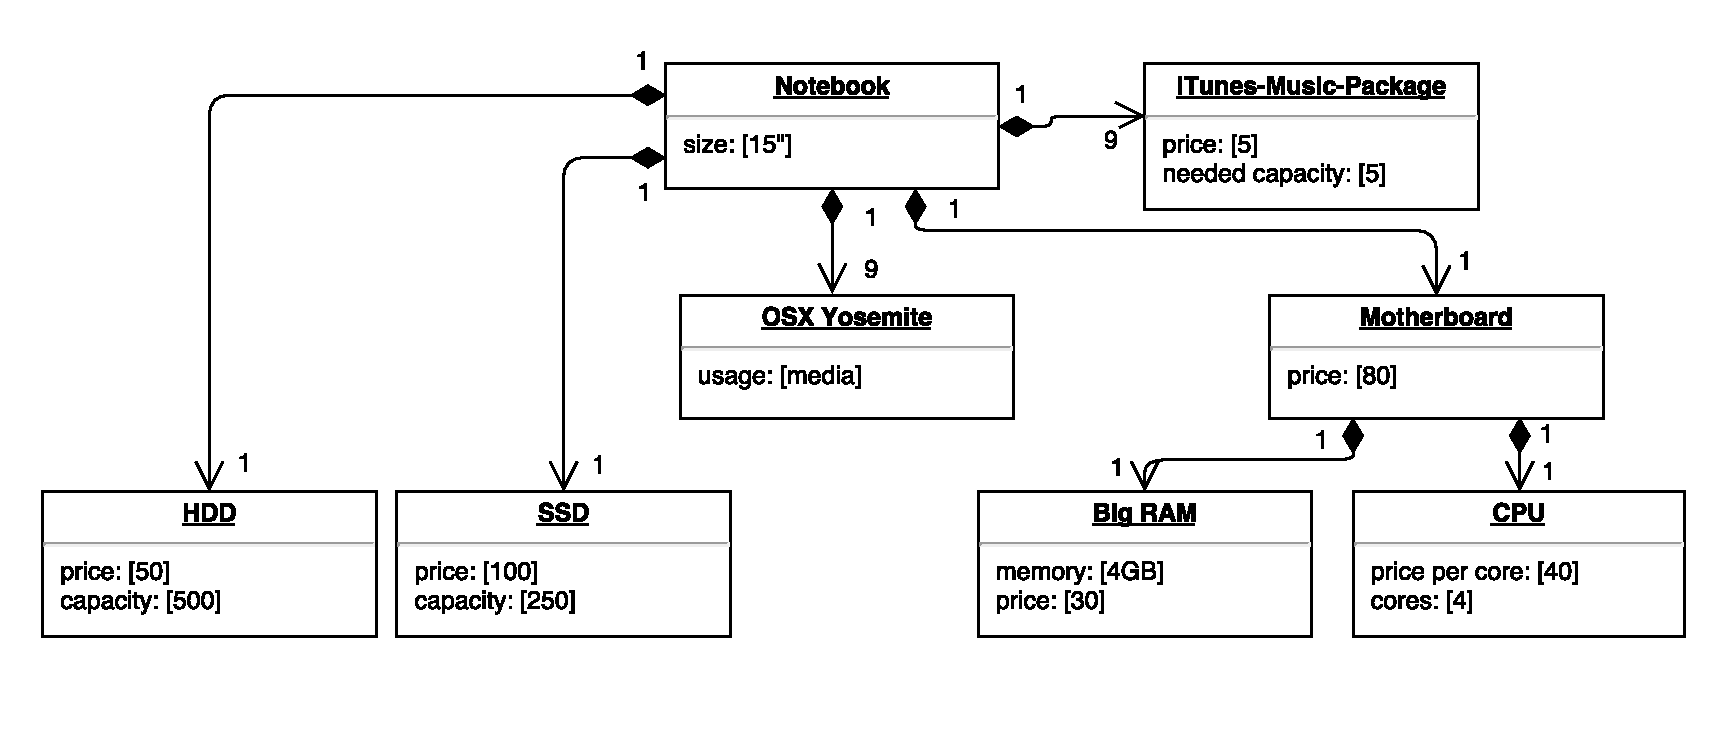
\includegraphics[width=1\linewidth]{Abbildungen/notebookInstanceUML.pdf}
	\captionof{figure}[Visualisierung einer Konfigurationslösung als UML-Instanz-Diagramm]{Visualisierung einer Konfigurationslösung als UML-Instanz-Diagramm}
	\label{fig:notebookInstanceUML}
\end{minipage}
\vspace{1em}

\subsection{Konfiguratoren}
\label{Konfigurationssysteme}
Konfiguratoren \glqq [...] führen den Abnehmer durch alle Abstimmungsprozesse, die zur Definition des individuellen Produktes nötig sind und prüfen sogleich die Konsistenz sowie Fertigungsfähigkeit der gewünschten Variante\grqq{} \citep{piller06}. Der erste Teil dieser Definition versteht den Konfigurationsprozess als eine Nutzerführung. Der zweite Teil der Definition entspricht der Charakterisierung als einen technischen Verarbeitungsprozess aus Kapitel \ref{begriffsuberblick}. Es muss also die technische- und die anwenderbezogene Sicht unterschieden werden. Aus technischer Sicht ist der Konfigurationsprozess die Verarbeitung einer Konfigurationsaufgabe. Aus Anwendersicht bezeichnet er den Abstimmungsprozess. Beides gehört zum Verantwortungsbereich des Konfigurators.

Nach \citet{piller06} besitzt ein Konfigurator drei Komponenten:
\begin{compactitem}
\item Die \textbf{Konfigurationskomponente} führt das Lösen von Konfigurationsaufgaben durch. Sie wird auch als Konfigurationsengine bezeichnet \citep{tactonProductOverview}.
\item Die \textbf{Präsentationskomponente} erstellt eine Konfigurationsdarstellung in zielgruppenspezifischer Form. Sie stellt die Schnittstelle für die Abstimmungsprozesse mit dem Anwender dar.
\item Die \textbf{Auswertungskomponente} präsentiert die Konfigurationslösung in einer Form, welche eine Interpretation der Variante außerhalb des Konfigurators erlaubt. Dies können z.B. Stücklisten, Konstruktionszeichnungen und Arbeitspläne sein.
\end{compactitem}

\subsubsection*{Konfiguratorarten}
Konfiguratoren für die Erhebung komplexer Anforderungen technischer Systeme  müssen von Konfiguratoren für den Einsatz im Rahmen der \ac{MC} unterschieden werden \citep{felferning14}. Erstere sind für den Experteneinsatz gedacht oder dienen nach \citet{piller06} als Vertriebskonfiguratoren der Unterstützung des Verkaufsgespräches. Letztere werden direkt vom Kunden in einer Company-to–Customer Beziehung genutzt und werden auch als \emph{Mass Customization Toolkits} bezeichnet. Die sogenannte \emph{Selbstkonfiguration} ist eine Voraussetzung für \ac{MC}, indem der zeitkonsumierende Prozess der Erhebung der Kundenbedürfnisse auf die Seite des Kunden verlagert wird \citep{piller06}

Konfiguratoren können bei allen in Abschnit \ref{Produktklassifizierung} genannten Produktionskonzepten zum Einsatz kommen, wobei der Konfigurationsprozess jeweils eine unterschiedliche Bedeutung hat. Bei \ac{PTO} hat der Konfigurator eine Katalogfunktion, indem er den Anwender bei der Auswahl eines fertigen Produkts aus einer Produktpalette unterstützt. Bei \ac{ATO} verhält sich der Konfigurator wie ein Variantengenerator, der den Anwender bei der Auswahl der richtigen Variante unterstützt. Dabei hat der Hersteller bereits alle möglichen Varianten vordefiniert. Daher werden diese als \emph{herstellerspezifisch} bezeichnet \citep{schomburg80}. Der Anwendungsfall bei \ac{MTO} ist ähnlich, jedoch wird durch die stärkere Einflussnahme des Kunden von \emph{kundenspezifischen} Varianten gesprochen \citep{schomburg80}. Außerdem unterstützt ein Konfigurator die regelbasierte Generierung von Konstruktionsdaten. Bei \ac{ETO} besteht ein erheblicher Neukonstruktionsbedarf. Dies widerspricht der Definition der Konfiguration als Routine Design aus Abschnitt \ref{begriffsuberblick} -- die Spezifikation der beteiligten Objekte ist nicht vollständig bekannt. Konfiguratoren können hier nur einen begrenzten Beitrag leisten. Aus dieser Erläuterung lässt sich ableiten, dass das Haupteinsatzgebiet von Konfiguratoren im \ac{ATO}/\ac{MTO} Umfeld liegt \citep{lutz11}.

\subsubsection*{Zusammenfassung}
In Abschnitt \ref{Produktklassifizierung} wurde dargestellt, wie bestimmte Produktionskonzepte die Herstellung individualisierter Produktvarianten bei gleichzeitiger Lagerfertigung ermöglichen. Produkte werden mit dem Ziel gestaltet, so individuell und auftragsunabhängig wie möglich zu sein. Damit wurde einer der Schlüsselfaktoren für die Ermöglichung der hybriden Wettbewerbsstrategie \ac{MC} erläutert. Diese verbindet die Vorteile effizienter Massenproduktion mit denen
der kundenspezifischen Einzelfertigung \citep{piller98}. \ac{MC} resultiert in Variantenvielfalt und damit in Produktkomplexität. In Abschnitt \ref{Produktkonfiguration} wurde die Funktionsweise von Konfiguratoren vorgestellt, mit welcher sie zur Beherrschung der Produktkomplexität beitragen.

\section{Webservices}
\label{Webservices}

Das \citet	{w3c04} definiert Webservices lose als:

\begin{quote}
\glqq [...] a software system designed to support interoperable machine-to-machine interaction over a network\grqq
\end{quote}

Die Definition schließt die Kommunikation heterogener Systeme ein. \glqq Zwischen Systemen\grqq{} differenziert gleichzeitig klar von der klassischen Verwendung eines Programms, bei der ein (menschlicher) Anwender mit einem System kommuniziert. \citet{tilkov11} bemerkt, dass Webservices damit sehr weich definiert sind -- \glqq nämlich eigentlich gar nicht\grqq{}. Fest steht, dass hier ein System einen Dienst als Schnittstelle anbietet, welche von einem Clienten über Webtechnologien ansprechbar ist. Webservices sind demzufolge eine Möglichkeit zur Realisierung von Integrationsszenarien webbasierter Systeme.

\vspace{1em}
\begin{minipage}{\linewidth}
	\centering
	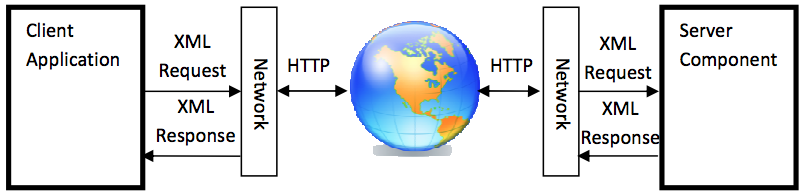
\includegraphics[width=0.7\linewidth]{Abbildungen/clientServerKommunikation.png}
	\captionof{figure}[Generische Client-Server Kommunikation bei Webservices]{Generische Client-Server Kommunikation bei Webservices}
	\label{fig:clientServerKommunikation.png}
\end{minipage}
\vspace{1em}

Abbildung \ref{fig:clientServerKommunikation.png} entspricht im wesentlichen der klassischen Client-Server Kommunikation im Web. Exemplarisch werden XML-Daten übertragen, was die zugrundeliegende Idee der Webservices illustriert -- die Übertragung anderer Daten als Webseiten mittels HTTP.

\citet{wilde11} reden von zwei etablierten \glqq Geschmäckern\grqq{} (flavors) in der Webservice-Welt: \emph{SOAP} und \emph{REST}. Die erste Geschmacksrichtung bedeutet Webservices \glqq auf Basis von SOAP, WSDL und den WS-*Standards - bzw. [...] deren Architektur\grqq{} \citep{tilkov11}. Hier wird ein XML-basierter Technologiestack beschrieben. REST hingegen ist ein Architekturstil, der 2000 in der Dissertation von Roy \citeauthor{fielding00} vorgestellt wurde. Der Versuch, beide Varianten direkt gegenüber stellen zu wollen, ist ein \glqq [...] klassischer Apfel-Birnenvergleich: ein konkretes XML-Format gegen einen abstrakten Architekturstil\grqq{} \citep{tilkov11}.

Vor einer detaillierteren Diskussion von SOAP und REST wird zur Einordnung eine grundlegende Unterscheidung der Ansätze vorgestellt. Gemeinsam ist beiden, dass HTTP als Transportprotkoll zur Übertragung der Frage (Request) verwendet wird, die vom Server (Response) beantwortert werden soll. Eine HTTP-Nachricht besteht aus einem Header und einem Entity-Body zur Übertragung von Daten. \citet{richardson07} haben zwei Leitfragen herausgearbeitet, die in diesem Zusammenhang von den jeweiligen Ansätzen unterschiedlich beantwortet werden: Wo in der Nachricht sagt der Client dem Service, mit welchen Daten (\emph{Fokusinformation}) was (\emph{Methodeninformation}) gemacht werden soll?

Die \textbf{Fokusinformation} sagt aus, für welche Datenelemente sich der Client interessiert (z.B. ein Artikel eines Onlineshops). Bei REST ist dies der \ac{URI} (d.h. der Webadresse) zu entnehmen (z.B. http://onlineshop.com/api/artikel/notebook). Bei SOAP steht diese Information in einer XML-Datei, welche im Entity-Body übertragen wird -- die sogenannte Payload. Die \textbf{Methodeninformation} sagt aus, was mit dem identifizierten Datenelement geschehen soll (z.B. \glqq erstelle einen neuen Notebook-Artikel\grqq{}). Bei REST steht dies im Methodenfeld des HTTP-Headers, bei SOAP abermals im Entity-Body. Daraus lässt sich als grundlegender Unterschied ableiten: SOAP verwendet HTTP nur als Transportprotokoll, REST auch dessen Ausdruckskraft \citep{wilde11}.

\subsection{SOAP}
Bei SOAP-Web Services wird ein \emph{\ac{RPC}} durchgeführt. Dabei handelt es sich um eine generelle Technik zur Realisierung von Systemverteilung. Ein System ruft die Funktion eines Systems aus einem anderen Adressraum auf. SOAP ist ein XML-basiertes Umschlagsformat, welches wiederum die Beschreibung eines Methodenaufrufs in XML-Form enthält. Bei SOAP-Webservices werden also \ac{RPC}s über HTTP getunnelt \citep{wilde11}. Das ist Konvention, aber keine Notwendigkeit. Der SOAP-Umschlag ist transportunabhängig, könnte also auch von anderen Protokollen als HTTP übertragen werden \citep{tilkov11}. Solange es sich bei dem Transportprotokoll um eine Webtechnologie handelt, wird die Webservicedefinition nicht verletzt.

Wie die Beschreibung des \ac{RPC} aussehen muss, definiert die \emph{\ac{WSDL}}. Jeder SOAP-basierte Service stellt eine maschinenverarbeitbare \ac{WSDL}-Datei bereit. Darin werden die aufrufbaren Methoden, deren Argumente und Rückgabetypen beschrieben. Außerdem werden die Schemata der XML-Dokumente festgehalten, welche der Service akzeptiert und versendet \citep{richardson07}.

Es existieren eine Vielzahl von Middleware-Interoperabilitätsstandards, die mit dem \glqq WS-\grqq{} Prefix versehen sind. Dabei handelt es sich um \glqq XML-Aufkleber\grqq{} für den SOAP-Umschlag, die HTTP-Headern entsprechen \citep{richardson07}. Sie erweitern die Ausdrucksmöglichkeit des SOAP-Formats \citep{wilde11}. Beispielsweise erlaubt \emph{WS-Security} die Berücksichtigung von Sicherheitsaspekten bei der Client-Server-Kommunikation. Eine Übersicht der existierenden Standards ist dem Wiki für Webservices \citep{webServiceWiki09} zu entnehmen.

\subsection{REST}
\label{REST}
\begin{quote}
\glqq Eine Architektur zu definieren bedeutet zu entscheiden, welche Eigenschaften das System haben soll, und eine Reihe von Einschränkungen vorzugeben, mit denen diese Eigenschaften erreicht werden können.\grqq{} \citep{tilkov11}
\end{quote}

Dies ist in der Dissertation von \citeauthor{fielding00} geschehen, in der REST als \emph{Architekturstil} definiert wird. Ein Architekturstil ist ein stärkerer Abstraktionsgrad als eine Architektur. Beispielsweise besitzt das Web eine Architektur, die eine HTTP-Implementierung von REST darstellt \citep{tilkov11}. Tatsächlich wurden die Einschränkungen von REST aber dem Web entnommen, indem \citeauthor{fielding00} es post hoc als lose gekoppeltes, dezentralisiertes Hypermediasystem konzeptualisiert hat \citep{wilde11} und dann von diesem Konzept abstrahierte. Einen Webservice nach dem REST-Architekturstil zu implementieren, passt ihn dem Wesen des Webs an und nutzt dessen Stärken \citep{tilkov11}.

Entsprechend \citeauthor{tilkov11}s Architekturdefinition werden im Folgenden die Einschränkungen von REST sowie die daraus resultierenden Eigenschaften besprochen.

\subsubsection{Einschränkungen}
\label{Einschränkungen}
Einschränkungen sind (in eigenen Worten) Implementierungskriterien. Während \citeauthor{fielding00} in seiner theoretischen Abhandlung explizit vier solcher Kriterien nennt, basiert die folgende Erläuterung auf der praxiserprobten Variante der Sekundärliteratur \citep{wilde11, tilkov11}.

\subsubsection*{Ressourcen mit eindeutiger Identifikation}
\glqq Eine Ressource ist alles, was wichtig genug ist, um als eigenständiges Etwas referenziert zu werden\grqq{} \citep{richardson07}. Identifiziert werden Ressourcen im Web durch \emph{\ac{URI}s}, die einen globalen Namensraum darstellen. Jede Ressource hat mindestens eine ID, eine ID kann jedoch nicht mehr als eine Ressource identifizieren. Es ist hervorzuheben, dass Ressourcen nicht das gleiche sind wie die Datenelemente aus der Persistenzschicht einer Anwendung. Sie befinden sich auf einem anderen Abstraktionsniveau \citep{tilkov11}.\vspace{0.3em}

Beispiel: Eine Warenkorbressource (d.h. ein virtueller Warenkorb) mit der ID '1024' hat die Adresse 'http://onlineshop.de/api/basket/1024'. Die einzelnen Warenkorbposition (d.h. die einzelnen Artikel im Warenkorb) sind jedoch nicht separat ansprechbar.

\citet{tilkov11} nimmt in diesem Zusammenhang eine Typisierung von Ressourcen vor. Von den sieben verschiedenen Ressourcentypen sind folgende im Rahmen der Arbeit interessant:
\begin{enumerate}
\item Bei einer \textbf{Projektion} wird die Informationsmenge verringert, indem eine sinnvolle Untermenge der Attribute einer abgerufenen Ressource gebildet wird. Zweck ist die Reduktion der Datenmenge.\vspace{0.2em}

Beispiel: Weglassen der Beschreibungstexte von Warenkorbpositionen.
\item Die \textbf{Aggregation} ist das Gegenteil. Hier werden Attribute unterschiedlicher Ressourcen zur Reduktion der Anzahl notwendiger Client-Server Interaktionen zusammengefasst.\vspace{0.2em}

Beispiel: Hinzufügen der Versandkosten beim Abruf des Warenkorbs.
\end{enumerate}
\subsubsection*{Hypermedia}
Hypermedia beschreibt das Prinzip verknüpfter Ressourcen. Dies ermöglicht es dem Clienten, neue Ressourcen zu entdecken und bestimmte Prozesse auszulösen \citep{wilde11}.

Beispiel (Ressource): Zu einer Warenkorbressource wird für jede enthaltene Warenkorbposition eine URI zur jeweiligen Detailseite (d.h. die Seite, auf welcher der Artikel einzeln präsentiert wird) hinzugefügt.

Beispiel (Prozess): Zur einer Bestellbestätigungsressource wird der zugehörige Stornierungslink hinzugefügt.

\subsubsection*{Standardmethoden/uniforme Schnittstelle}
Oben wurde beschrieben, dass jede Ressource durch (mindestens) eine ID identifiziert wird. Jede URI unterstützt dabei den gleichen Methodensatz, welche mit den HTTP-Methoden korrespondieren. Übertragen auf die objektorientierte Programmierung bedeutet das: Jede Klasse implementiert das gleiche Interface. Folgende Teilmenge der neun verfügbaren HTTP-Methoden finden in der Literatur am häufigsten Erwähnung \citep{richardson07, tilkov11, wilde11}:
\begin{enumerate}[a.]
\item [\textbf{GET:}] Das Abholen einer Ressource.\vspace{0.2em}

Beispiel: GET an 'http://onlineshop.com/api/artikel/notebook' holt die Notebook-Ressource.
\item [\textbf{PUT:}] Das Anlegen oder Aktualisieren einer Ressource. Je nachdem, ob unter dieser URI bereits eine Ressource existiert.\vspace{0.2em}

Beispiel: PUT an 'http://onlineshop.com/api/artikel/notebook' erzeugt eine Notebook-Ressource unter dieser Adresse, wenn noch keine andere besteht.
\item [\textbf{POST:}] Bei POST werden zwei Bedeutungen unterschieden. Im engeren Sinne bedeutet es das Anlegen einer Ressource unter einer URI, die vom Service bestimmt wird. Im weiteren Sinne kann durch Post ein Prozess ausgelöst werden.\vspace{0.2em}

Beispiel (im engeren Sinne): POST an 'http://onlineshop.com/api/artikel/notebook' mit einer JPG-Datei als Payload erzeugt eine neues Bild für die Notebook-Ressource. Die Bild-Ressource bekommt jedoch die URI 'http://onlineshop.com/api/images/notebook'.

Beispiel (im weiteren Sinne): POST an 'http://onlineshop.com/api/artikel/notebook' löst eine Bestellung für das Notebook aus.
\item [\textbf{Delete:}] Das Löschen einer Ressource.\vspace{0.2em}

Beispiel: DELETE an 'http://onlineshop.com/api/artikel/notebook' löscht die Notebook-Ressource.
\end{enumerate}

\vspace{1em}
\begin{minipage}{\linewidth}
	\centering
	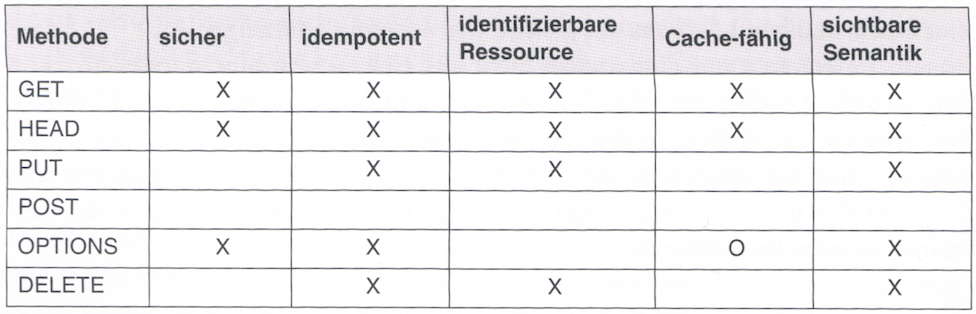
\includegraphics[width=0.7\linewidth]{Abbildungen/restMethoden.png}
	\captionof{table}[HTTP-Methoden und ihre Eigenschaften]{HTTP-Methoden und ihre Eigenschaften\footnote{Relevante Attribute im Rahmen der Arbeit: \glqq Sicher\grqq{} bedeutet nebenwirkungsfrei, d.h. kein Ressourcenzustand ändert sich durch diese Methode. \glqq Idempotent\grqq{} bedeutet, dass das Resultat der Methode bei Mehrfachausführung das gleiche ist. \glqq Identifizierbare Ressource\grqq{} bedeutet, dass die URI garantiert eine Ressource identifiziert.}
	(Quelle: \citet{tilkov11})}
	\label{tab:restMethoden}
\end{minipage}
\vspace{1em}

Tabelle \ref{tab:restMethoden} fasst die Eigenschaften der Methoden aus der HTTP-Spezifikation 1.1 zusammen. Die Implementierung einer Methode muss dem erwarteten Verhalten aus dieser Spezifikation entsprechen. Die Praxis zeigt, dass nur die Methoden unterstützt werden, die für die jeweilige Ressource sinnvoll sind. Tabelle \ref{tab:restMethoden} macht außerdem klar, dass es für POST keinerlei Garantien gibt. \citet{richardson07} sehen bei der Verwendung des POST im weiteren Sinne (prozessbezogen) eine Verletzung der uniformen Schnittstelle. Dies wird damit begründet, dass das Resultat des Prozesses, der durch POST ausgelöst wird, der API-Beschreibung des Webservices und nicht der HTTP-Spezifikation zu entnehmen ist. Das schafft eine Abhängig von der Webserviceimplementierung, die gerade durch die uniforme Schnittstelle vermieden werden soll.

\subsubsection*{Ressourcen und Repräsentationen}
Beschreibt die Darstellungen einer Ressource in einem definierten Format. Der Client bekommt nie die Ressource selbst, sondern nur eine Repräsentation derer zu sehen. In der Praxis hat sich durchgesetzt, eine serialisierte Variante eines Objektes als JSON-Objekt zur Verfügung zu stellen \citep{tilkov11}.

Beispiel: Bereitstellung einer Bestellbestätigung als PDF und HTML.

\subsubsection*{Statuslose Kommunikation}
Bei REST soll ein serverseitig abgelegter, transienter, clientspezifischer Status über die Dauer eines Requests hinweg vermieden werden. Der Service benötigt also nie Kontextinformationen zur Bearbeitung eines Requests.

Beispiel: Ein Warenkorb wird nicht in einem Sessionobjekt, sondern als persistentes Datenelement gehalten.

\subsubsection{REST-Konformität}
\label{REST-Konformität}
Diese Auflistung legt folgende Frage nahe: Ist ein Webservice nur dann REST-konform, wenn alle Kriterien erfüllt werden? Was ist mit einem Webservice, der allen Einschränkungen gerecht wird, jedoch Ressourcen nur in Form von JSON repräsentiert (ein Verstoß gegen die Forderung nach unterschiedlichen Repräsentationen)? Aus diesem Grund existiert das \glqq Richardson Maturity Model\grqq{}, welches die abgestufte Bewertung eines Webservices nach dessen REST-Konformität erlaubt. Es wird während der Auswertung in Kapitel \ref{Fazit} vorgestellt und zur Evaluierung der Implementierung genutzt.

\subsubsection{Eigenschaften}
\label{REST-Eigenschaften}
Aus den vorgestellten Kriterien resultieren folgende Eigenschaften \citep{tilkov11},  welche die Vorteile REST-basierter Webservices gegenüber der SOAP-Konkurrenz darstellen \citep{richardson07}:

\begin{compactitem}
\item [\textbf{Lose Kopplung:}] Beschreibt isolierte Systeme mit größtmöglicher Unabhängigkeit, die über Schnittstellen miteinander kommunizieren. Hierzu tragen die Standardmethoden bei.
\item [\textbf{Interoperabilität:}] Beschreibt die Möglichkeit der Kommunikation von Systemen unabhängig von deren technischen Implementierung. Dies ergibt sich durch die Festlegung auf Standards. Bei der Anwendung von REST auf Webservices sind dies Webstandards (z.B. HTTP, URIs).
\item [\textbf{Wiederverwendbarkeit}:] Jeder Client, der die Schnittstelle eines REST-basierten Services verwenden kann, kann auch jeden anderen beliebigen REST-basierten Service nutzen - vorausgesetzt, das Datenformat wird von beiden Seiten verstanden.
\item [\textbf{Performance und Skalierbarkeit}:] Webservices sollen schnell antworten, unabhängig von der Anzahl der Anfragen in einem definierten Zeitraum. Dies wird durch die Cachebarkeit (siehe HTTP-Methodenspezifikation in Tabelle \ref{tab:restMethoden}) und Zustandslosigkeit erreicht. Da der Service keinen clientspezifischen Kontext aufbauen muss, müssen aufeinanderfolgende Requests nicht vom gleichen Server beantwortet werden.
\end{compactitem}

\subsubsection*{Zusammenfassung}
REST ist ressourcenorientiert, während SOAP aufgrund von \ac{RPC}s methodenorientiert ist. Die Umsetzung von REST ist nicht an technische Voraussetzungen gebunden, vielmehr müssen eine Reihe von Kriterien erfüllt werden. Das Implementierungswerkzeug von REST sind Funktionen, die auf HTTP-Requests an definierte URIs reagieren, diese verarbeiten und mit einer HTTP-Nachricht beantworten können. Bei SOAP ist HTTP nur das Transportprotokoll. Die Verarbeitung des Inhalts erfordert einen weiteren Technologiestack.

\section{eCommerce}
\label{eCommerce}

Im Folgenden wird durch die Charakterisierung des Begriffs \emph{eCommerce} ein Anwendungsrahmen für Onlineshops (\emph{eShops}) hergestellt. Deren softwaretechnische Umsetzung wird durch \emph{eShop-Systeme} realisiert. Durch eine Kategorisierung der Systeme nach Anbieterstrategie wird abschließend die Menge der Open-Source-Lösungen für eine Konfiguratorintegration identifiziert.

\subsection{Anwendungsrahmen}
\label{eCommerce:Anwendungsrahmen}
eShops gehören zur Domäne des elektronischen Handels (eCommerce). eCommerce ist \glqq die elektronisch unterstützte Abwicklung von Handelsgeschäften auf der Basis des Internet\grqq{} \citep{schwarze02}. Je nachdem, welche Marktpartner an dem Handelsgeschäft teilnehmen, werden verschiedene Formen des eCommerce unterschieden. Die in Tabelle \ref{tab:eCommerceGrundformen} fett hervorgehobenen Varianten werden von \citet{meier12} als \glqq die zwei Geschäftsoptionen des eCommerce\grqq{} bezeichnet -- \emph{\ac{B2C}} und \emph{\ac{B2B}}. Bei \ac{B2C} erfolgt der Handel von Produkten und Dienstleistungen zwischen Unternehmen und Endverbraucher, bei \ac{B2B} zwischen Unternehmen.

\vspace{1em}
\begin{minipage}{\linewidth}
	\centering
	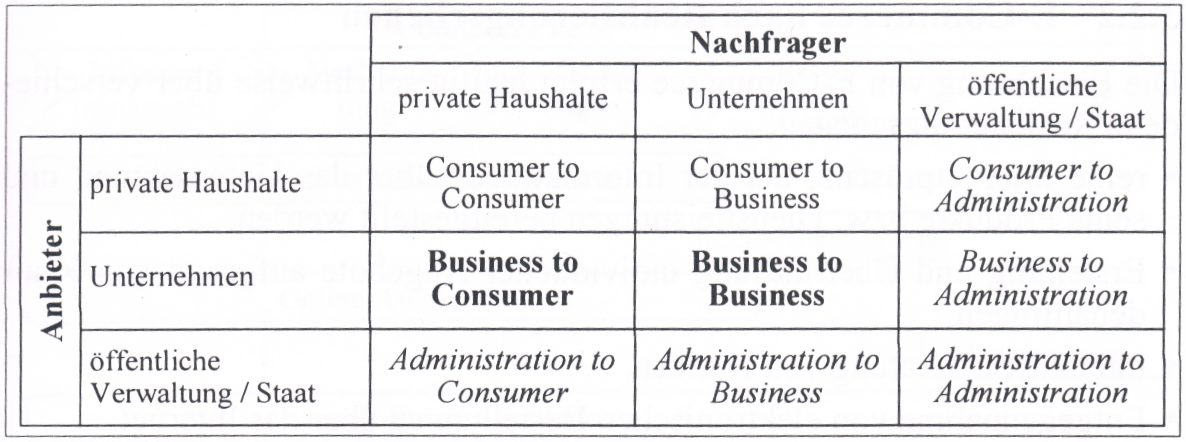
\includegraphics[width=0.6\linewidth]{Abbildungen/eCommerceGrundformen.png}
	\captionof{table}[Grundformen des eCommerce]{Grundformen des eCommerce nach Marktpartnern (Quelle: \citet{schwarze02})}
	\label{tab:eCommerceGrundformen}
\end{minipage}
\vspace{0.1em}

Für die Umsetzung von eCommerce existieren unterschiedliche Geschäftsmodelle. \citet{timmers98} nennt elf verschiedene Formen, wobei eShops eine davon sind. Es handelt sich dabei um ein \glqq Geschäftsmodell der Angebotsveröffentlichung, bei dem ein Anbieter seine Waren oder Dienstleistungen über das Web den Nachfragern offeriert\grqq{} \citep{bartelt00}.

Ein eShop bildet den traditionellen Einkaufsvorgang nach: Kunden können mittels einer Katalog- oder Suchfunktion über den Produktbestand navigieren (\emph{Artikellisting}). Produkte können ausgewählt und ausführliche, mit Medien angereicherte Beschreibungen abgerufen werden (\emph{Detailseite}). Wunschartikel werden einem virtuellen \emph{Warenkorb} hinzugefügt. Ist die Produktauswahl abgeschlossen, begibt sich der Kunde zur \glqq Kasse\grqq{}, wo die Zahlungsmodalitäten erledigt werden (\emph{Bestellung}) \citep{boles00}.

Ein eShop beschreibt das Geschäftsmodell, jedoch noch nicht dessen Umsetzung als Softwaresystem. Dieses wird als eShop-System bezeichnet \citep{boles00} und im Folgenden behandelt.

\subsection{eShop-Systeme}
\label{eShop-Systeme}
\glqq eShop-Systeme sind Software-Systeme, die den Aufbau, die Verwaltung und den Einsatz von eShops unterstützen\grqq{} \citep{boles00}. Abbildung \ref{fig:eShopGrobarchitektur} zeigt die Grobarchitektur eines eShop-Systems nach \citet{meier12}. Darin wird die Unterteilung zwischen Storefront und Backfront deutlich, welche in der Terminologie realer Shopsysteme als Front- und Backend bezeichnet werden \citep[vgl.][]{shopwareDoku}. Das Frontend ist der Interaktionsraum der Kunden, das Backend der administrative Bereich des Shopbetreibers.

\vspace{1em}
\begin{minipage}{\linewidth}
	\centering
	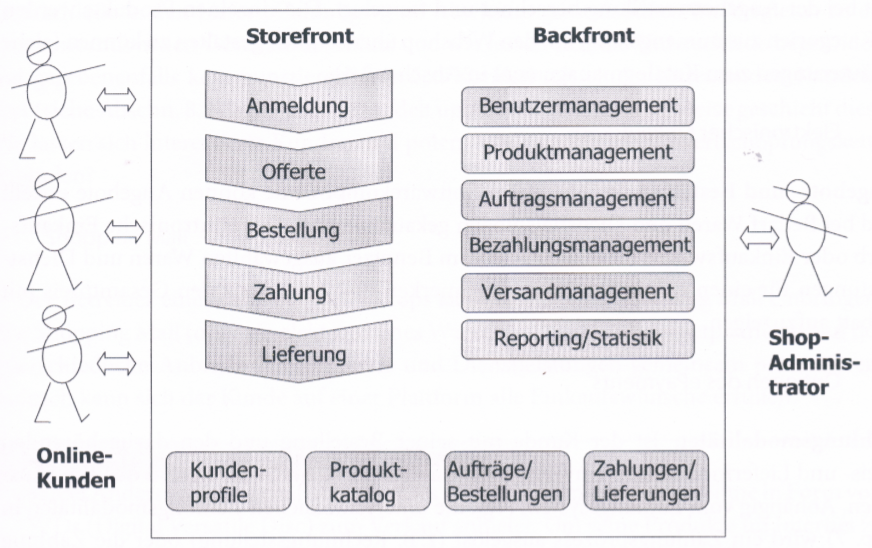
\includegraphics[width=0.7\linewidth]{Abbildungen/eShopGrobarchitektur.png}
	\captionof{figure}[Grobarchitektur eines eShop-Systems]{Grobarchitektur eines eShop-Systems (Quelle: \citet{meier12})}
	\label{fig:eShopGrobarchitektur}
\end{minipage}
\vspace{0.2em}

Die Hauptaufgaben eines eShop-Systems sehen \citet{boles00} in den Bereichen \emph{Merchandising} (z.B. Management von hierarchisch strukturierten Produktkatalogen, Beeinflussung des Shopdesigns), \emph{Auftragsbearbeitung} (z.B. Festlegung der Abarbeitungs-Pipeline, Integration von Bezahlverfahren) und \emph{Sonstiges} (z.B. Kopplung mit externen ERP-Systemen). Der konkrete Funktionsumfang hängt vom gewählten eShop-System ab.

Die Systeme sind nach Strategie der Anbieter kategorisierbar, wie im Folgenden dargestellt wird.

\subsubsection*{Open-Source}
Der Quellcode von Open-Source-Systemen ist kostenlos verfügbar. Daher bieten sie völlige Gestaltungsfreiheit, aber keinen Herstellersupport. Die Dokumentationen sind schwächer und der Funktionsumfang geringer als bei kostenpflichtigen Alternativen. Andererseits existieren Communities, die Unterstützung bieten und die Entwicklung von Erweiterungen vorantreiben \citep{stahl15}.

Open-Source bedeutet nicht per se, dass die Systeme ohne Kostenaufwand einsetzbar sind. Beim kommerziellen Handel der modularen Erweiterungen auf shopspezifischen Stores liegt eine der Erlösquellen der Open-Source-Strategie (siehe der \glqq Addon Marketplace\grqq{} der PrestShop SA\footnote{http://addons.prestashop.com} oder das \glqq Extension Directory\grqq{} der Opencart Limited\footnote{http://www.opencart.com/index.php?route=extension/extension}).

\subsubsection*{Kauf-Lösungen}
Kauf-Lösungen werden kostenpflichtig lizensiert \citep[z.B.][]{shopwarePricing}. Sie bieten Herstellersupport, zusätzliche Dienstleistungen (z.B. Installation des Shops) und einen höheren Funktionsumfang (z. B. Schnittstellen zu verschiedenen Warenwirtschaftssystemen oder Zahlungsdienstleistern) \citep{stahl15}. Die Hersteller bieten verschiedene Editionen mit teilweise erheblichen Preisunterschieden an\footnote{Beispiel: die Preisdifferenz der \emph{Magento Enterprise Edition} zu \emph{Enterprise Premium} liegt bei über 35.000 \$ \citep[vgl][]{fwpShop}}.

Im Rahmen eines Dual-License-Modells ist eine Open-Source \emph{Community Edition} Teil des Editionsspektrums \citep{t3n14} (siehe das Shopangebot der \citet{magentoShops}, \citet{shopwarePricing} oder \citet{oxidShops}). Durch den offenen Quellcode existiert auch hier der Handel modularer Erweiterungen, von dem auch die kostenpflichtigen Varianten profitieren (siehe der \emph{Plugin Store} der shopware AG\footnote{http://store.shopware.com/}). Die Codebasis aller Editionen ist gleich. Daher kann später zu einer Kauf-Lösung migriert werden. Das bietet Flexibilität für wachsende Shopanforderungen.

\subsubsection*{Miet-Shops}
Miet-Shops entsprechen einer Cloud-Lösung als \emph{Software-as-a-Service} (z.B. \citet{stratoWebshops}, \citet{shopify15}). Die technische Infrastruktur wird vom Provider zur Verfügung gestellt. Systemwartung, Bereitstellung der Shopsoftware und Hosting werden unter dem Mietpreis abgerechnet. \citet{stahl15} bewerten diese Variante als Einstiegslösung mit geringer Gestaltungsfreiheit.

\subsubsection*{Eigenentwicklungen}
Wenn die Standardsysteme die Anforderungen nicht erfüllen, eignen sich Eigenentwicklungen für individuelle Bedürfnisse \citep{stahl15, graf14}.

Aus dieser Darstellung sind die (zumindest initial) kostenfreien Varianten ersichtlich: Reine Open-Source eShop-Systeme sowie die Community-Editionen der Dual-License Modelle. Eine Anbieterübersicht ist \citet{t3n14} zu entnehmen. Eine Kategorisierung der Systeme nach Anforderungsklassen ist \citet{graf14} zu entnehmen.

\section*{Zusammenfassung}
Im vorangegangenen Kapitel wurde das theoretische Fundament für die Arbeit gelegt. Durch die Aufstellung eines Anwendungsrahmens wurde ein wirtschaftlicher Kontext für Konfiguratoren im Allgemeinen geschaffen. Daraufhin wurde die Konfiguration als Prozess zur Variantenbestimmung besprochen. Dieser Prozess eignet sich besonders für Produkte, deren Bestandteile nicht beliebig kombiniert werden können. Daraufhin wurden Konfiguratoren als Systeme vorgestellt, die eine Nutzerschittstelle zur Konfiguration anbieten und die Entscheidungen des Anwenders im Rahmen von Konfigurationsaufgaben verarbeiten. Die Diskussion von Webservices hat ergeben, dass REST und SOAP die Instrumentierung des Webs für Integrationsszenarien ermöglichen.

Im Zusammenhang mit den Geschäftsoptionen des eCommerce lässt sich eine genauere Aussage über den Anwendungsbezug von Konfiguratoren in eShops machen. Der Konfigurationsprozess im B2C wird durch den Endverbraucher durchgeführt, entspricht also der Selbstkonfiguration. Im B2B ist die Konfiguration komplexerer Systeme möglich, z.B. durch die Bedienung von Vertriebskonfiguratoren durch ausgebildetes Personal. 

\chapter{Analyse}
\label{section:Analyse}

Nachdem in Kapitel \ref{Grundlagen} Konfiguratoren und eShop-Systeme unabhängig von konkreten Systemumsetzungen betrachtet wurden, findet nun eine Analyse von existierenden softwaretechnischen Implementierungen statt. Festgelegt durch die Lino GmbH kommt der \emph{Tacton Produktkonfigurator} zum Einsatz. Es wird zunächst dessen spezifisches Konfigurationsmodell analysiert. Daraufhin wird eine Konfiguratoranwendung in Form des Vertriebskonfigurators \emph{TCsite} vorgestellt. Aus der Analyse dieses Systems kann eine genauere Aussage über die in Frage kommenden eShop-Systeme für die Integration getroffen werden. Daraufhin wird ein System festgelegt und mit dessen Betrachtung fortgefahren. Davon ausgehend findet im Fazit des Kapitels ein Grobkonzept der jeweiligen Verantwortungsbereiche der Systeme im Integrationsszenario statt.

\section{Tacton Produktkonfigurator}

Die Tacton Systems AB (Tacton) wurde 1998 als Spin-Off des Schwedischen Instituts für Informatik (SICS) gegründet \citep{tactonProductOverview}. In der Forschungseinrichtung wurde als Resultat der Untersuchungen in den Bereichen \glqq Wissensbasierte Systeme\grqq{} und \glqq Künstliche Intelligenz\grqq{} der Tacton Produktkonfigurator entwickelt. Dieser interaktive Konfigurator ist die Basis der verschiedenen Produkte der Firma. Tacton bietet Lösungen in den Bereichen \glqq Vertriebskonfiguration\grqq{} und \glqq Design Automation\grqq{} (Automatisierung der Konstruktion in CAD-Systemen) \citep{tactonAbout}.

\subsection{Konfigurationsmodell}
\label{tactonKonfigurationsmodell}
Das in Abschnitt \ref{wissenrepraesentation} vorgestellte Visualisierungskonzept abstrahiert Konfigurationswissen in einen Struktur- und einen Regelteil. Im Tacton-Konfigurationsmodell wird ebenfalls abstrahiert, jedoch in andere Domänen \citep{tactonModeling}:

\begin{enumerate}[(a)]
\item \label{strukturinformation} \textbf{Strukturinformation}: Wie ist das Produkt hierarchisch aufgebaut?
\item \label{komponenteninformation} \textbf{Komponenteninformation}: Aus was ist es aufgebaut?
\item \label{constraintinformationen} \textbf{Constraint-Informationen}: Wann ist das Produkt korrekt?
\item \label{ausfuehrungsinformationen} \textbf{Ausführungsinformationen}: Welche Fragen bekommt der Nutzer während des Konfigurationsprozesses in welcher Reihenfolge gestellt?
\end{enumerate}

Dabei sind zwei Sachverhalte feststellbar:
\begin{enumerate}[(1)]
\item \label{enum:componentsConfiguration} Typisch für einen modellbasierten Konfigurator wird Produktwissen und Problemlösungswissen bei der Wissensmodellierung separiert \citep{felferning14}.

Beispiel: Ein Constraint, der die Kompatibilität bestimmter Betriebssysteme mit einer bestimmten Anzahl Prozessorkerne ausdrückt, soll wirken, auch ohne die konkreten CPU-Typen (z.B. \glqq Intel i7\grqq{}) zu kennen.

Darum ist die Rede von \emph{generischen Constraints} -- sie beziehen sich auf alle \emph{Komponenten} (erläutert im folgenden Kapitel) eines Typs \citep{felferning14}.
\item \label{enum:execution} Gemäß \eqref{ausfuehrungsinformationen} wird im Konfigurationsmodell auch die Nutzerinteraktion festgelegt. Damit geht der Funktionsumfang eines Tacton-Modells über die Definition aus Abschnitt \ref{begriffsuberblick} hinaus.
\end{enumerate}

Bei der UML-Wissensrepräsentation aus Abschnitt \ref{wissenrepraesentation} wurden die Domänen \eqref{strukturinformation} und \eqref{komponenteninformation} als Diagramm sowie \eqref{constraintinformationen} als Tabelle ausgedrückt. Tacton wählt eine andere Aufteilung. \eqref{komponenteninformation} wird unter dem Begriff  \emph{Components} umgesetzt, \eqref{strukturinformation} und \eqref{constraintinformationen} werden unter dem Begriff \emph{Configuration} zusammengefasst. Components und Configuration setzen gemeinsam den Sachverhalt \eqref{enum:componentsConfiguration} um und werden im Folgenden besprochen. Daraufhin wird die \emph{Execution} besprochen, welche Sachverhalt \eqref{enum:execution} darstellt.


\subsubsection{Components und Configuration}

\vspace{1em}
\begin{minipage}{\linewidth}
	\centering
	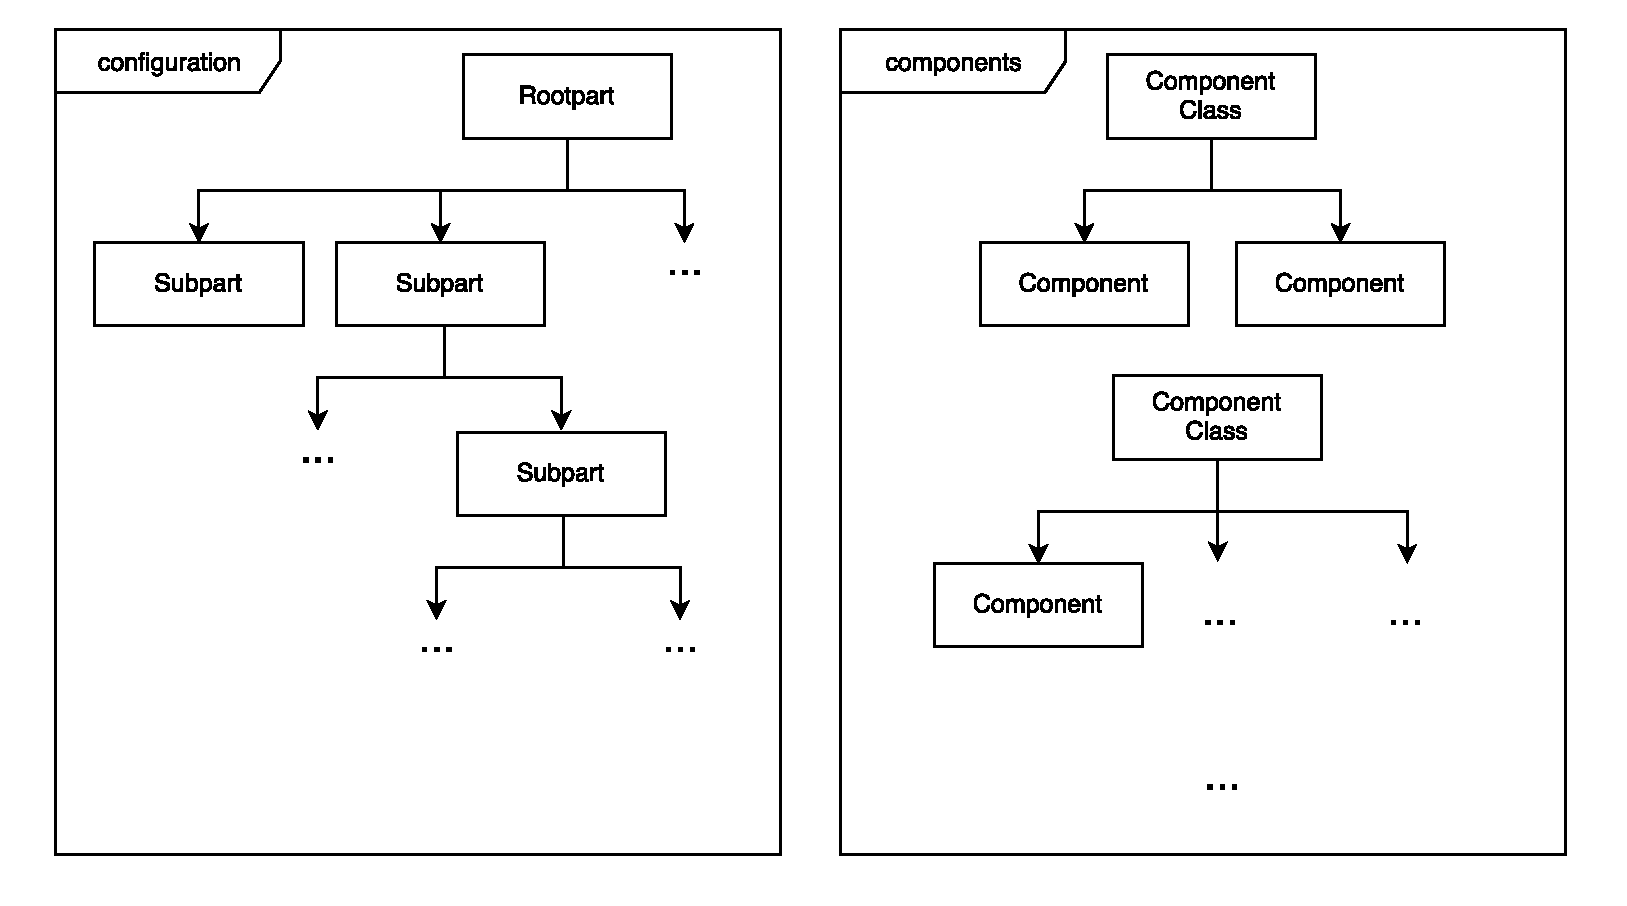
\includegraphics[width=0.75\linewidth]{Abbildungen/tactonModellHighLevel.pdf}
	\captionof{figure}[High-Level-Architektur des Tacton-Konfigurationsmodells]{High-Level-Architektur des Tacton-Konfigurationsmodells}
	\label{fig:tactonModellHighLevel}
\end{minipage}
\vspace{0.3em}

Abbildung \ref{fig:tactonModellHighLevel} zeigt das High-Level-Konzept der Modellarchitektur. Unter \emph{configuration} wird die Produktstruktur als hierarchischer Baum von \emph{Part}-Objekten dargestellt. Jeder Part kann Constraints enthalten, die sich auf den Knoten selbst und alle seine Kinder beziehen. Ein Part ist ansonsten nur ein Komponentenplatzhalter. Noch ist keine Information darüber hinterlegt, welches Bauteil dort eigentlich verkörpert wird. Abbildung \ref{fig:tactonModellHighLevelNotebook} veranschaulicht das Konzept am Notebook-Beispiel.

\vspace{1em}
\begin{minipage}{\linewidth}
	\centering
	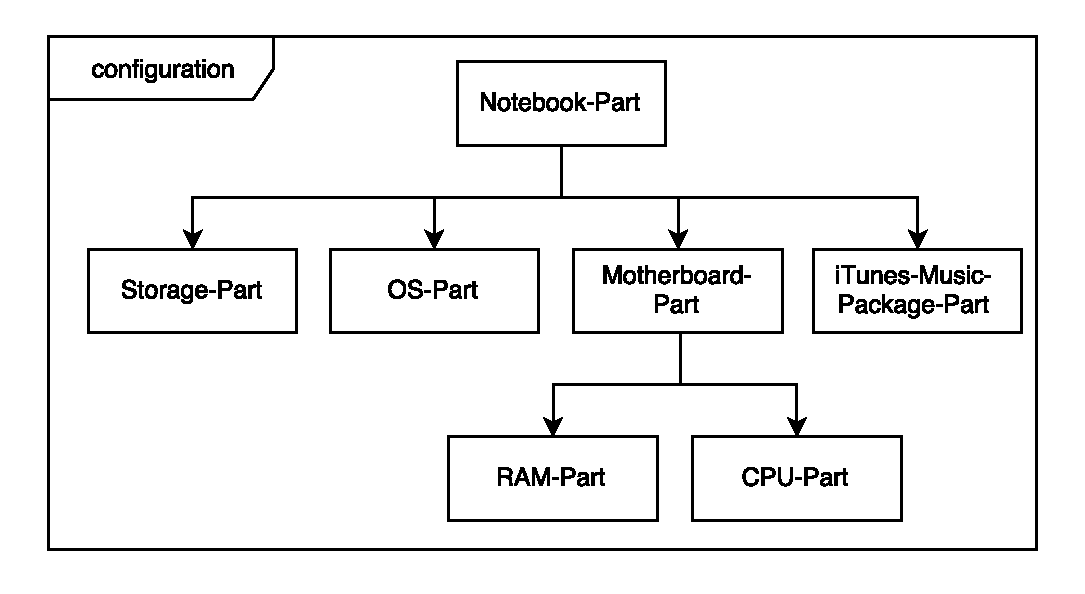
\includegraphics[width=0.6\linewidth]{Abbildungen/tactonModellHighLevelNotebook.pdf}
	\captionof{figure}[Part-Struktur der exemplarischen Notebook-Konfiguration]{Part-Struktur der exemplarischen Notebook-Konfiguration}
	\label{fig:tactonModellHighLevelNotebook}
\end{minipage}
\vspace{0.3em}

Die Informationen über die eben erwähnten Bauteile (d.h. Komponententypen) werden isoliert unter \emph{components} definiert (siehe Abbildung \ref{fig:tactonModellHighLevel}). Ein Bauteil wird in \emph{Component Classes} und \emph{Components} abstrahiert. Das ist analog zu Komponententypen, die in einer Generalisierungsbeziehung zueinander stehen (siehe Kapitel \ref{wissenrepraesentation}). Hier wurde eine Terminologie gewählt, die Supertyp und Subtyp unterscheidbar machen. Eine \emph{Component Class} (z.B. ein 'RAM') wird durch Eigenschaften beschrieben, die als \emph{Features} bezeichnet werden. Jedes Feature besitzt einen Namen (z.B. 'memory') und einen Wertebereich (z.B. ['2GB', '4GB']), welche als \emph{Domain} bezeichnet wird. Wertebereiche können Integer, Float, Boolean, andere Component Classes oder selbstdefinierte Enumerationen sein. Components (z.B. eine 'SSD') sind das, was eine Component Class (z.B. ein 'Storage') konkret sein kann. Sie übernehmen alle Features der übergeordneten Component Class und besitzen konkrete Werte (\emph{Values}) aus dem jeweiligen Wertebereich.

\vspace{1em}
\begin{minipage}{\linewidth}
	\centering
	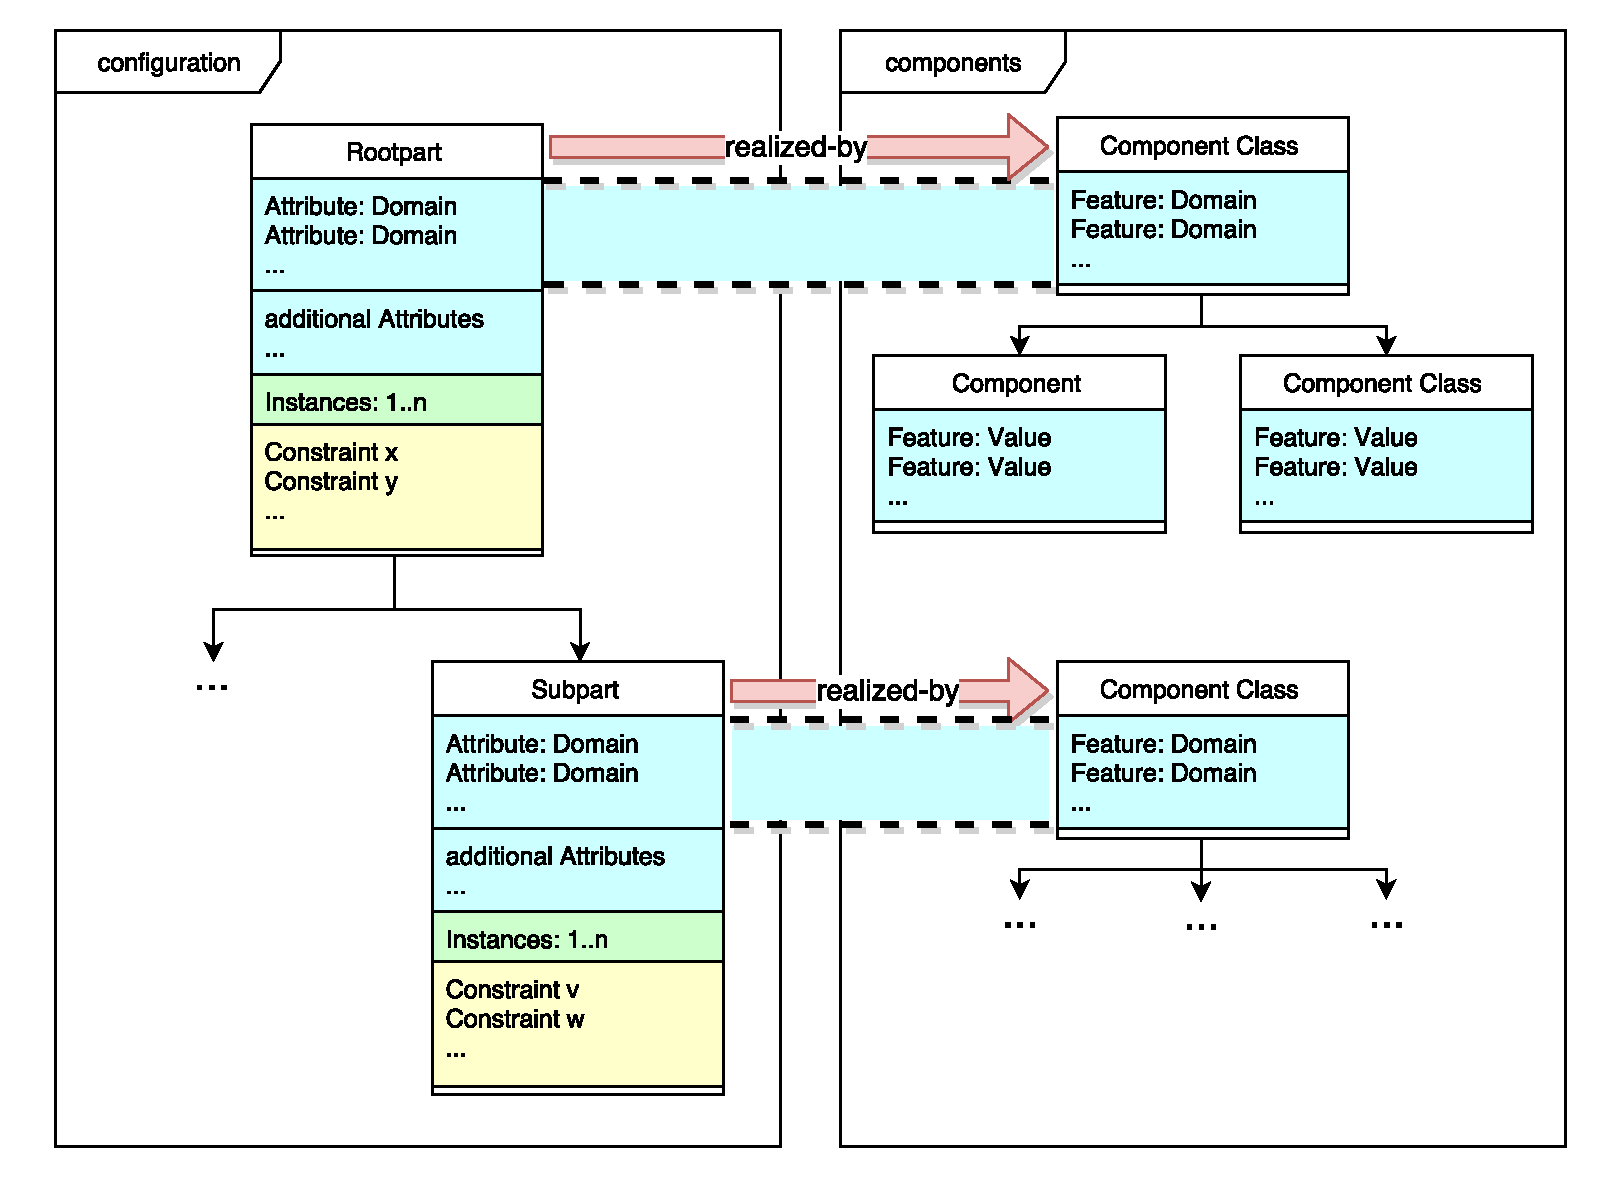
\includegraphics[width=0.8\linewidth]{Abbildungen/tactonModellLowLevel.pdf}
	\captionof{figure}[Zuordnung von Parts und Component Classes]{Zuordnung von Parts und Component Classes}
	\label{fig:tactonModellLowLevel}
\end{minipage}
\vspace{0.2em}

Abbildung \ref{fig:tactonModellLowLevel} zeigt die Zuordnung zwischen Parts und Component Classes via Verzeigerung. Dabei wird einem Part eine Component Class durch eine \emph{realyzed by}-Beziehung zugeordnet. Dem Part werden dabei die Features der entsprechenden Component Class vererbt (türkis dargestellt). Nur werden sie zur besseren Differenzierung beim Part nicht mehr als Features, sondern als \emph{Attributes} bezeichnet. Für einen Part können auch noch zusätzliche Attribute definiert werden (als 'additional Attributes' dargestellt), falls notwendig. Die Angabe \emph{Instances} (grün dargestellt) entspricht den Kardinalitäten in Abschnitt \ref{fig:tactonModellLowLevel}. \emph{Constraints} (gelb dargestellt) werden als logische Ausdrücke formuliert. Sie bestehen aus Attributwerten, die mit mathematischen Zeichen in Relation gebracht werden.

\vspace{1em}
\begin{minipage}{\linewidth}
	\centering
	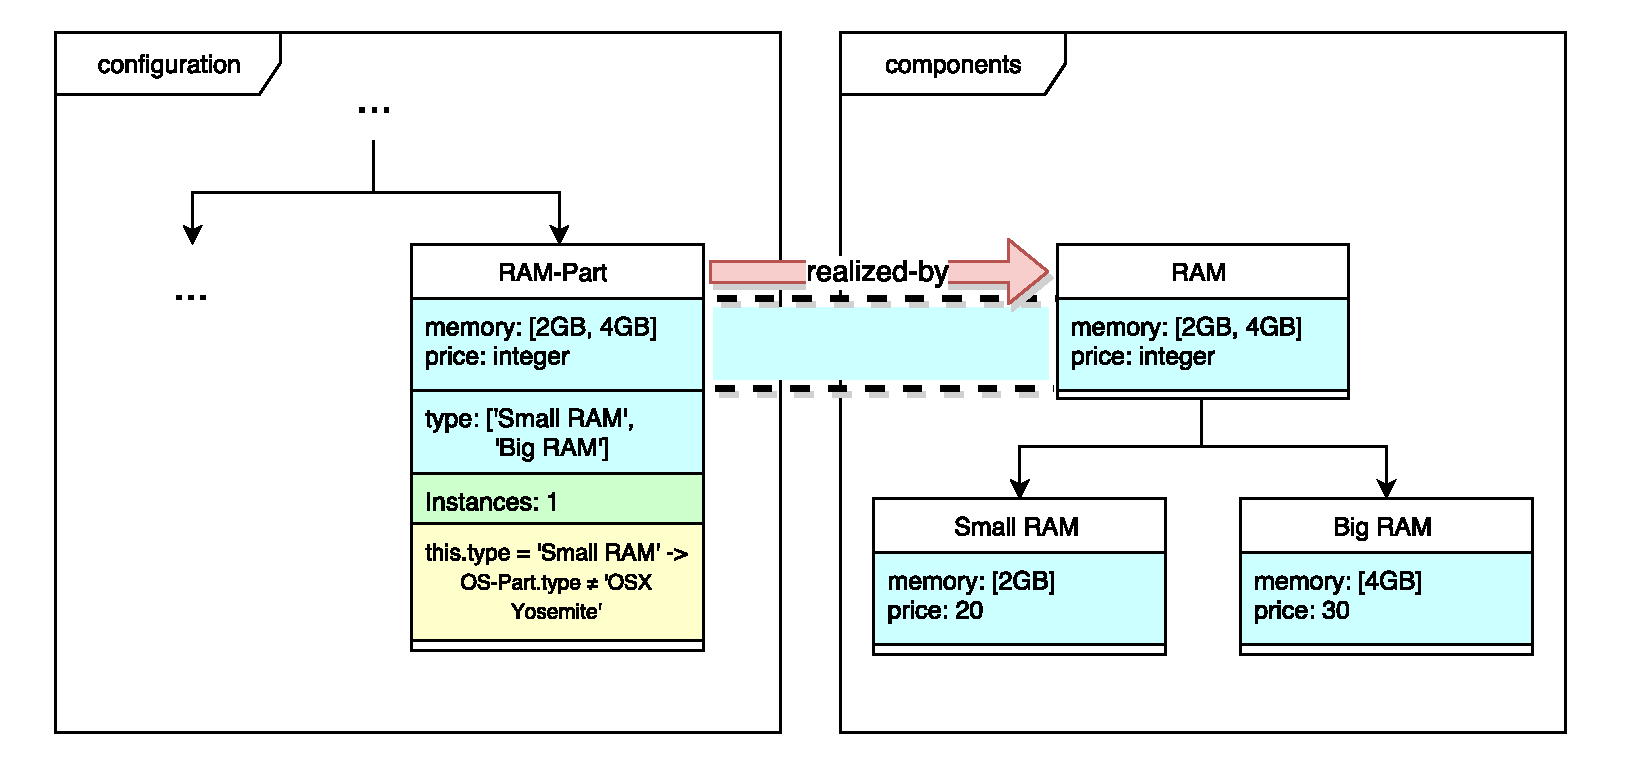
\includegraphics[width=0.9\linewidth]{Abbildungen/tactonModellLowLevelNotebook.pdf}
	\captionof{figure}[Zuordnung von Part und Component Class der exemplarischen Notebook-Konfiguration]{Zuordnung von Part und Component Class der exemplarischen Notebook-Konfiguration}
	\label{fig:tactonModellLowLevelNotebook}
\end{minipage}

Abbildung \ref{fig:tactonModellLowLevelNotebook} veranschaulicht den Sachverhalt anhand eines Ausschnitts der exemplarischen Notebook-Konfiguration. Der Part übernimmt die Attribute 'memory' und 'price'. Das zusätzliche Attribut 'type' kapselt beispielsweise die Bezeichnungen der jeweiligen Components als Enumeration (z.B. ['Small RAM', ‘Big RAM']). Der Constraint veranschaulicht exemplarisch, wie die Inkompatibilität mit dem Betriebssystem vom Typ 'OSX Yosemite' formuliert wird.

\subsubsection{Execution}
\label{Execution}
Es wurde dargestellt, wie das Konfigurationswissen im Tacton Konfigurationsmodell definiert wird. Dadurch ist aber noch nicht gesagt, welche Entscheidungen ein Nutzer während der Konfiguration treffen kann. Nicht jeder Part und nicht jedes Attribut müssen eine relevante Wahl darstellen. Vielleicht sollen dem Nutzer sogar Fragen auf einem anderen Abstraktionsniveau als auf Komponentenebene gestellt werden. Statt \glqq Soll eine HD oder eine SSD als Festplatte in das Notebook eingebaut werden?\grqq{} kann auch gefragt werden: \glqq Möchten Sie viel Speicherplatz oder einen schnellen Speicherzugriff?\grqq.

Der Abstimmungsprozess durch den Anwender wird unter dem Begriff \emph{Execution} definiert. Dabei wird nicht einfach nur eine Menge an Optionen festgelegt, die dem Nutzer am Ende als Liste präsentiert werden. Stattdessen werden die Optionen hierarchisch strukturiert.

\vspace{1em}
\begin{minipage}{\linewidth}
	\centering
	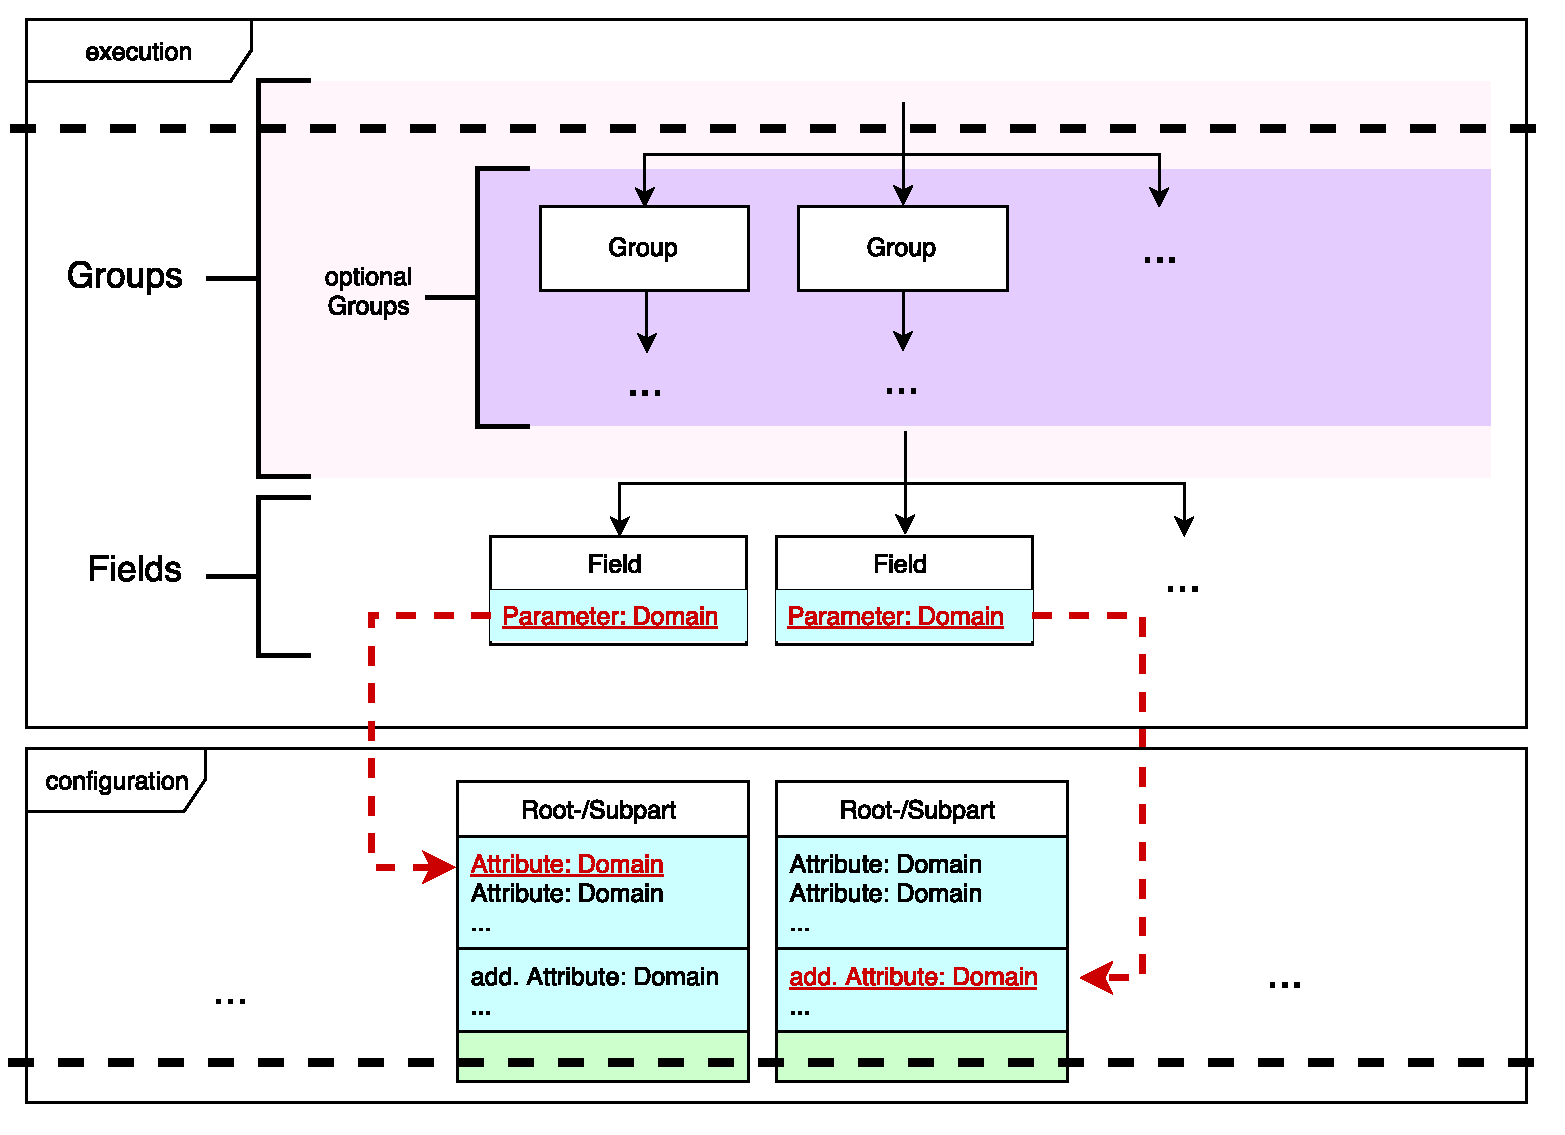
\includegraphics[width=0.8\linewidth]{Abbildungen/tactonModellExecutionShort.pdf}
	\captionof{figure}[Ausschnitt der generischen Execution-Struktur]{Ausschnitt der generischen Execution-Struktur}
	\label{fig:tactonModellExecution}
\end{minipage}
\vspace{0.3em}

Abbildung \ref{fig:tactonModellExecution} zeigt einen Ausschnitt der generischen Struktur der Execution als Baum. Die vollständige Darstellung ist Anhang \ref{app:tactonModellExecutionLong} zu entnehmen und wichtig zum weiteren Verständnis. Abbildung \ref{fig:tactonModellExecutionNotebook} veranschaulicht das Konzept durch eine mögliche Execution-Struktur der exemplarischen Notebook-Konfiguration.

\begin{enumerate}[1.]
\item Die Wurzel wird als \textbf{Applikation} bezeichnet. Sie beinhaltet die Gesamtheit aller Optionen.

Beispiel: Eine Notebook-Konfiguration.
\item Die nächste Knotenebene wird als \textbf{Steps} bezeichnet. Sie legen fest, in welcher Reihenfolge die Optionen präsentiert werden. Das ist in verschiedenen Fällen sinnvoll. Zum Beispiel dann, wenn komplexe Probleme in mehrere Schritte unterteilt oder Werte für spätere Schritte gesetzt werden sollen.

Beispiel: In Step 1 legt der Anwender eine Preisgrenze fest. In Step 2 wird die technische Spezifikation getroffen, wobei die Preisgrenze aus Step 1 nicht überschritten werden darf.
\item Nun folgen $1..n$ Knotenebenen, die als \textbf{Groups} bezeichnet werden. Sie fassen Optionen zu logischen Einheiten zusammen. Es werden zwei Typen unterschieden:
\begin{enumerate}
\item[\textbf{Top-Level-Groups}:] Die oberste Group-Ebene ist obligatorisch.

Beispiel: Eine 'Speicher'-Gruppe in Step 2.
\item[\textbf{optional Groups}:] Die Unterteilung in weitere Gruppen ist optional.

Beispiel: Unter der 'Speicher'-Gruppe wird eine weitere Gruppe namens 'Massenspeicher' angelegt, um sie vom 'RAM' zu unterscheiden.
\end{enumerate}
\item \textbf{Fields} sind die Blätter des Execution-Baums. Sie sind das, worüber der Anwender Optionen wählt. Alle darüber liegenden Knoten haben den Fields nur eine Ordnungsstruktur gegeben.

Aus Anwendersicht besteht ein Field aus einer Beschreibung und einem Interaktionselement. Aus technischer Sicht repräsentiert ein Field einen \emph{Parameter} mit einem Wertebereich (\emph{Domain}), aus welchem ein Wert (\emph{Value}) gewählt wird. Die Parameter stammen aus den Attributen der Parts. Das Wählen einer Option bedeutet also letztendlich das Wählen des Wertes eines Part-Attributs.

Je nach Interaktionselement wird in unterschiedliche Feldtypen unterschieden:
\begin{enumerate}[(a)]
\item [\textbf{Menu:}] Wahl aus einem Wertebereich, z.B. via Dropdownmenü.

Beispiel \glqq Massenspeicher\grqq{}:\\
Parameter = 'Storage-Part.type', Domain = ['HD', 'SSD']

Beispiel \glqq CPU-Kerne\grqq{}:\\
Parameter = 'CPU-Part.cores', Domain = [1..4].
\item [\textbf{Number:}] Eingabe eines eigenen Wertes in ein Textfeld.

Beispiel \glqq Preisgrenze\grqq{} (Eingabe in Schritt 1):\\
 Parameter = 'Notebook-Part.maxPrice', Domain = [integer]
\item [\textbf{Label:}] Anzeige eines Wertes aus Informationsgründen.

Beispiel \glqq Aktueller Preis\grqq{} (Anzeige in Schritt 2):\\
Parameter = 'Notebook-Part.price', Domain = [integer]
\end{enumerate}
\end{enumerate}

Die Feldtypen \emph{Menu} und \emph{Number} haben gemein, dass der Anwender einen Wert aus einem Wertebereich festlegt. Beim \emph{Menu} ist dieser Wertebereich eine Menge vordefinierter Optionen, bei \emph{Number} ein Zahlenbereich, wobei der konkrete Wert vom Anwender selbst eingegeben wird. Um die Formulierung kurz zu halten, werden im Folgenden sowohl die ausgewählte Option als auch der eingegebene Wert unter dem Begriff \emph{Eingabeparameter} zusammengefasst.

Das Modell wird in einem XML-basierten Format mit der Dateiendung '.tcx' gespeichert. Die Entwicklung einer solchen Datei wird von entsprechenden Programmen unterstützt. Hierfür kann zum Beispiel \glqq TCstudio\grqq{} genutzt werden, welches eine grafische Oberfläche zur Modellentwicklung bietet \citep{tactonAbout}.

\begin{minipage}{\linewidth}
	\centering
	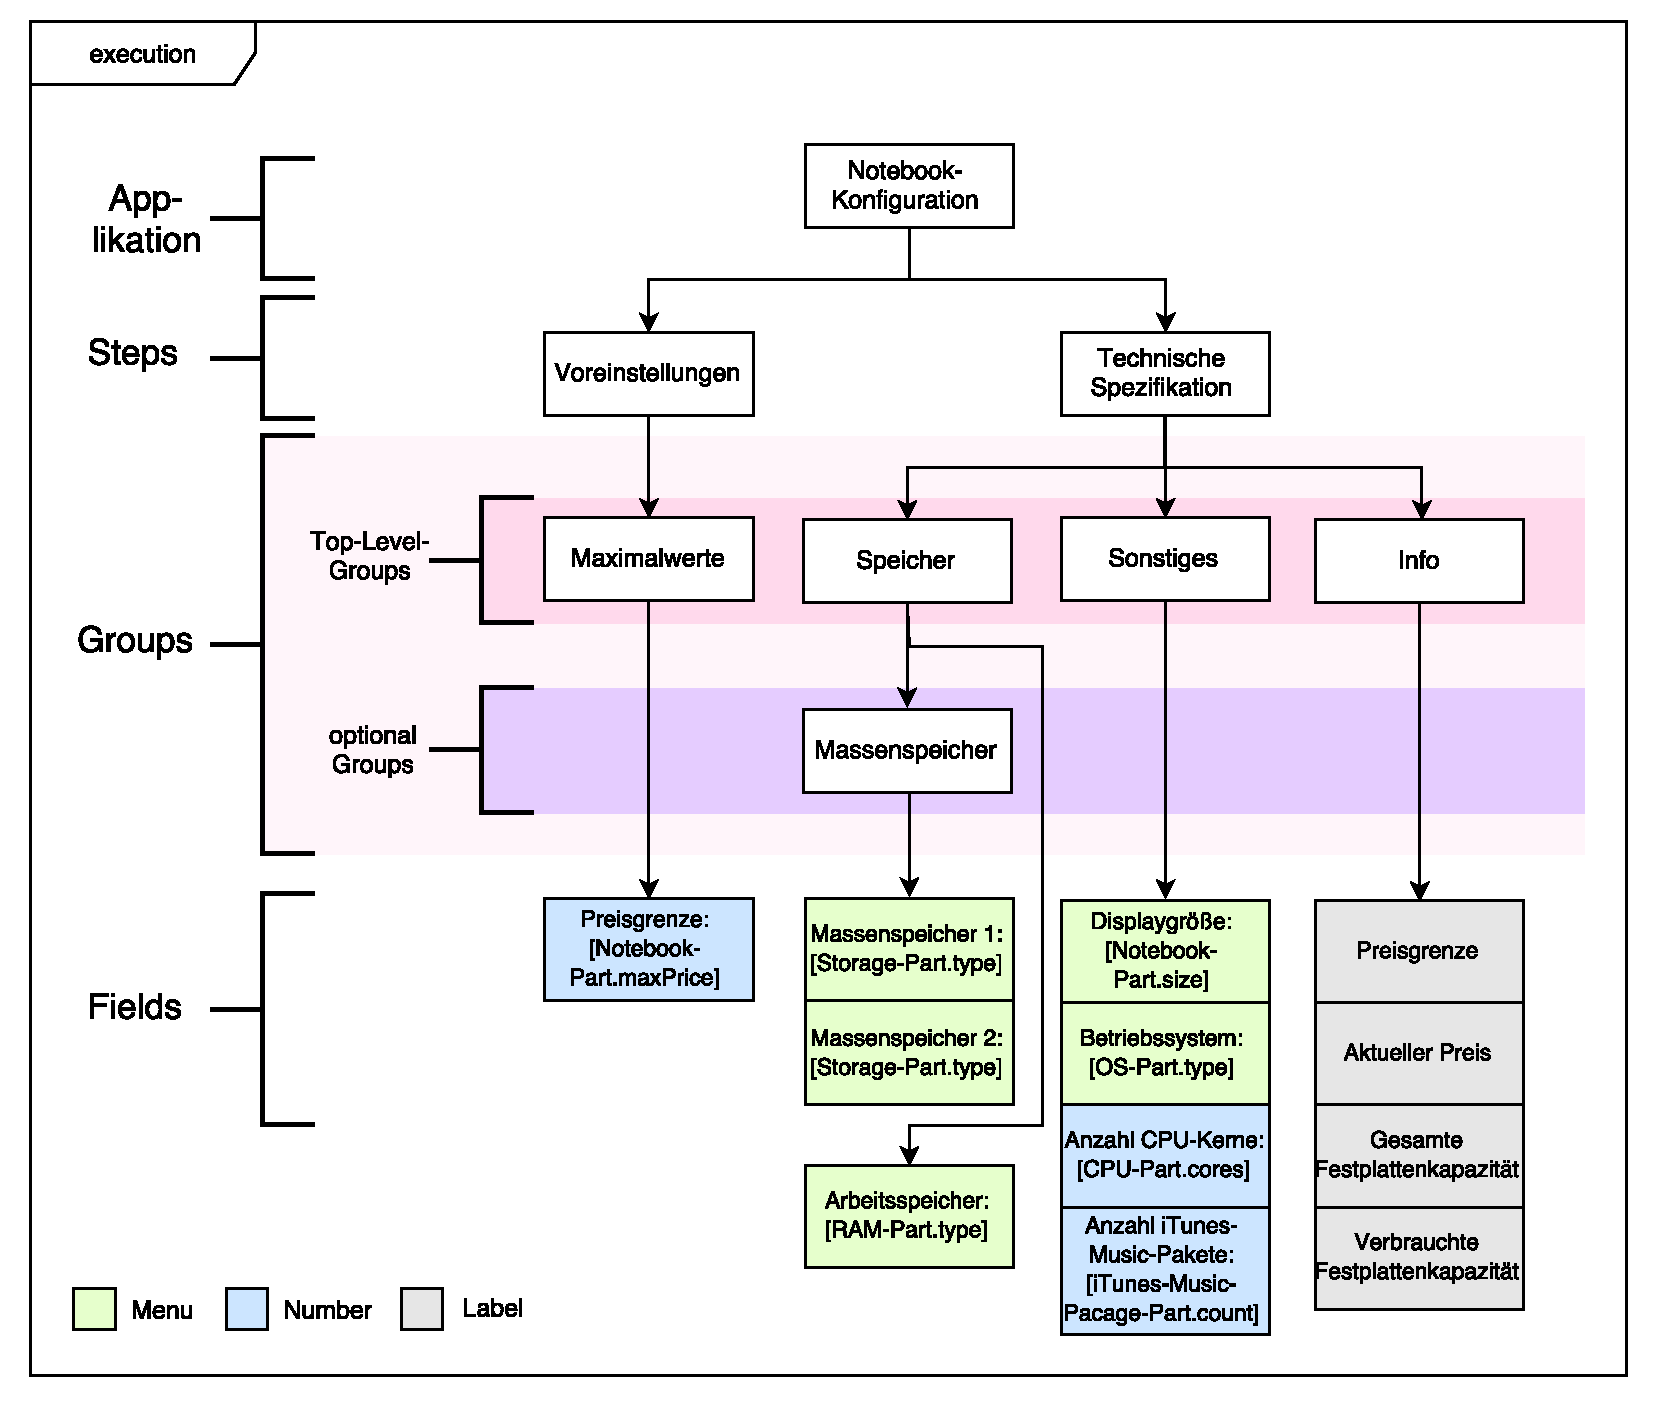
\includegraphics[width=0.8\linewidth]{Abbildungen/tactonModellExecutionNotebook.pdf}
	\captionof{figure}[Mögliche Exection-Struktur der exemplarischen Notebook-Konfiguration]{Mögliche Exection-Struktur der exemplarischen Notebook-Konfiguration}
	\label{fig:tactonModellExecutionNotebook}
\end{minipage}
\vspace{0.3em}

\subsubsection*{Zusammenfassung}
Das Tacton-Modellierungskonzept wurde vorgestellt. Neben dem Konfigurationswissen werden darin auch die Optionen des Anwenders definiert. Diese werden durch Steps in eine Reihenfolge gebracht und durch Groups logisch gegliedert. Über Felder wählt der Anwender Optionen. Der Feldtyp \emph{Number} ermöglicht die Eingabe eines eigenen Wertes. So werden Komponenten definiert, die nach Kundenanforderung konstruiert oder gefertigt werden müssen. Entsprechend der vorgestellten Produktklassifizierung in Kapitel \ref{Produktklassifizierung} bildet das Konfigurationsmodell so auch \ac{MTO}-Produkte ab.

Das Konfigurationsmodell definiert die Interaktionsstruktur. Diese muss jedoch noch in Form eine Konfigurationsoberfläche dargestellt werden. Neben anderen Funktionalitäten realisiert TCsite eine solche Darstellung. Die Anwendung wird im folgenden analysiert.

\subsection{TCsite}
\label{TCsite}
\emph{TCsite} ist ein webbasierter Vertriebskonfigurator. Er könnte theoretisch von Endkunden genutzt werden, bildet aber nicht den Einkaufsprozess eines eShops gemäß Kapitel \ref{eCommerce:Anwendungsrahmen} nach. Stattdessen handelt es sich um eine \textbf{CPQ}-Lösung (\textbf{C}onfigure-\textbf{P}rice-\textbf{Q}uote). Das bedeutet: der Anwender wird durch die Konfiguration geführt, was in einer Preiskalkulation resultiert, woraus wiederum ein Angebot erstellt wird. Eine unmittelbare Bestellung und Zahlungsabwicklung ist nicht vorgesehen. Der Anwendungsbereich liegt also im B2B \citep{tactonAbout}.

Technisch betrachtet ist TCsite eine Webanwendung. Der serverseitige Programmcode ist in Java verfasst. Im Lieferumfang sind \emph{Apache Tomcat} als Application Server sowie \emph{TCserver} enthalten. TCserver ist das, was gemäß Kapitel \ref{Produktkonfiguration} als eigentlicher Konfigurator bezeichnet wird. Er beherbergt die \emph{Konfigurationsengine}. Damit ist das System gemeint, welches Konfigurationsaufgaben verarbeitet \citep{tactonTCsiteHandbook}. Abbildung \ref{fig:tcsiteHighLevel} veranschaulicht die High-Level-Architektur des Standardsetups.

\vspace{1em}
\begin{minipage}{\linewidth}
	\centering
	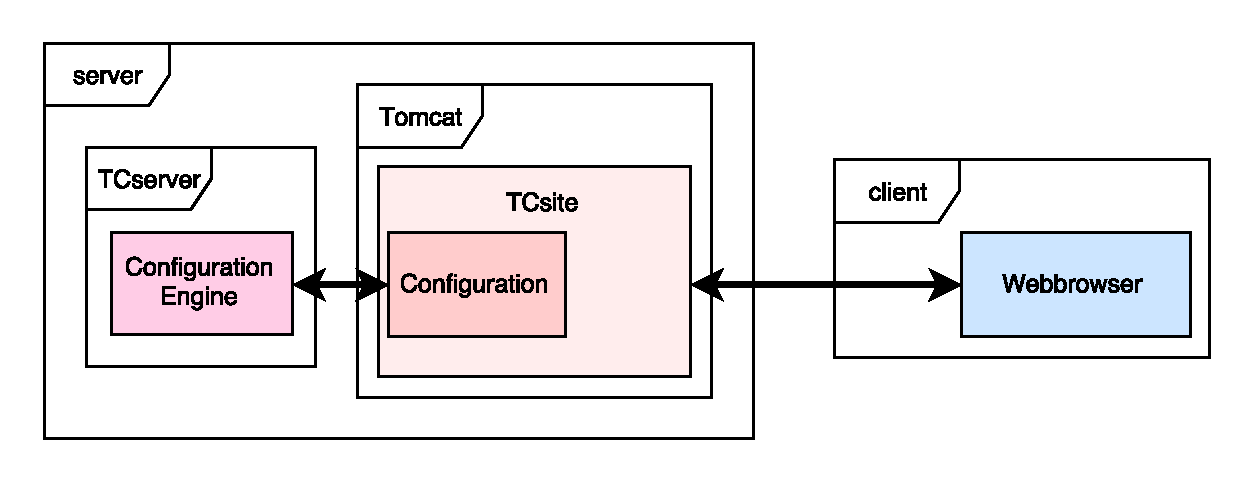
\includegraphics[width=0.7\linewidth]{Abbildungen/tcsiteHighLevel.pdf}
	\captionof{figure}[High-Level-Architektur von TCsite]{High-Level-Architektur von TCsite}
	\label{fig:tcsiteHighLevel}
\end{minipage}

\subsubsection{Architektur}
\label{TCsiteArchitektur}

Abbildung \ref{fig:tcsiteLowLevel} visualisiert die offene Schichtenarchitektur von TCsite. Offen bedeutet, dass jede Schicht mit allen darunter liegenden Schichten kommunizieren kann. Das Fundament bildet die Persistenzschicht. Sie realisiert die Datenhaltung. Die Plattform bildet ein \ac{API} mit den Basisfunktionalitäten für die darüber liegenden Schichten. Die Module realisieren jeweils eine der drei Oberflächenbereiche der Anwendung. Außerdem bieten sie Services und Erweiterungspunkte für die oberste Schicht -- die Plugins. Durch diese kann die Funktionalität von TCsite individuell erweitert werden \citep{tactonTCsiteDevelopmentManual}.

\vspace{1em}
\begin{minipage}{\linewidth}
	\centering
	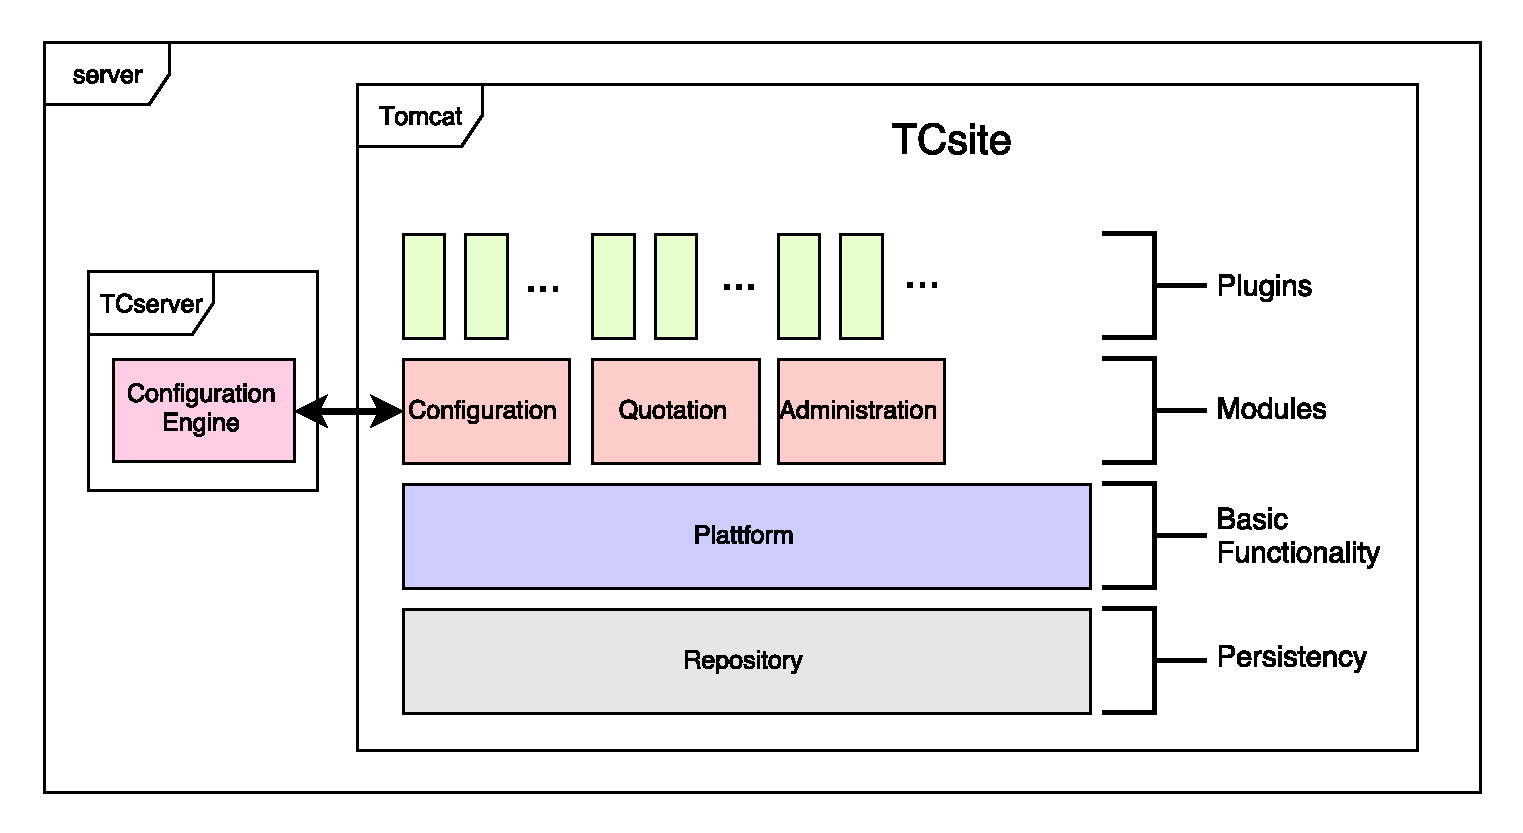
\includegraphics[width=0.7\linewidth]{Abbildungen/tcsiteLowLevel.pdf}
	\captionof{figure}[Schichtenarchitektur von TCsite]{Schichtenarchitektur von TCsite}
	\label{fig:tcsiteLowLevel}
\end{minipage}
\vspace{0.3em}

Im Folgenden werden die Architekturkomponenten einzeln vorgestellt.

\subsubsection*{Repository}
Das \emph{Repository} bietet eine Datenbank sowie ein Reihe von Funktionen zum Lesen und Schreiben der TCsite-Objekte. Es ist in einen lokalen und einen globalen Speicher strukturiert. Wird ein Objekt erstellt oder geöffnet, geschieht die Bearbeitung immer auf einer Arbeitskopie in dem für jeden Nutzer spezifischen lokalen Speicher. Änderungen sind solange für andere Nutzer unsichtbar. Erst ein \glqq Commit\grqq{} sorgt für die nutzerübergreifende Sichtbarkeit im globalen Speicher. Dabei wird eine Revisionshistorie über Objektänderungen geführt, so dass alte Zustande wieder abrufbar sind \citep{tactonTCsiteDevelopmentManual}.

\subsubsection*{Plattform}
Die Plattform bietet keine eigene Oberfläche, sondern bildet eine \ac{API} mit grundlegenden Funktionalitäten für die darüberliegenden Schichten \citep{tactonTCsiteDevelopmentManual}. 

\subsubsection*{Administration}
Dieses Modul bildet die Administrationsoberfläche, dargestellt in Anhang \ref{app:tcsiteAdministration}. Hier werden Einstellungen getroffen und Verwaltungsaspekte realisiert. Dazu gehört zum Beispiel die Verwaltung der Nutzergruppen und Produkte.

Die Nutzergruppen definieren, welche Rechte ein TCsite-User hat. Standardmäßig verfügbar sind die Nutzergruppen \glqq Standarduser\grqq{}, \glqq Systemadministrator\grqq{} und \glqq Integrationsuser\grqq{}. Letzterer Typ dient der Authentifizierung bei der Kommunikation mit externen Systemen, zum Beispiel bei einem Integrationsszenario. Bildlich gesprochen personifiziert jede externe Webanfrage einen Gast, der die Maske des Integrationsusers aufgesetzt und dessen Rechte bekommt \citep{tactonTCsiteDevelopmentManual}.

\vspace{1em}
\begin{minipage}{\linewidth}
	\centering
	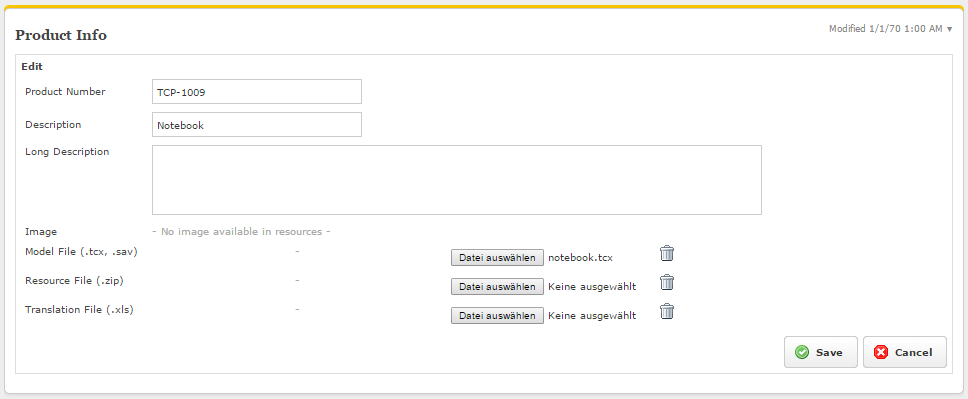
\includegraphics[width=0.95\linewidth]{Abbildungen/tcsiteAdministrationProduct.PNG}
	\captionof{figure}[Detailsansicht eines Produktes aus dem Produktkatalog]{Detailsansicht eines Produktes aus dem Produktkatalog}
	\label{fig:tcsiteAdministrationProduct}
\end{minipage}
\vspace{0.3em}

Außerdem wird hier der Produktkatalog verwaltet. Abbildung \ref{fig:tcsiteAdministrationProduct} zeigt die Detailansicht eines Produkts. Die Darstellung macht deutlich, dass neben Produktbeschreibungen auch Dateien hinterlegt werden. Wird eine Modelldatei hochgeladen, ist das Produkt konfigurierbar. Ressourcen, wie z.B. Bilder oder eine Übersetzungsdatei können ergänzend hinzugefügt werden \citep{tactonTCsiteReferenceManual}. Entsprechend der Definition eines Konfigurationsmodells in Kapitel \ref{Produktkonfiguration} werden so nicht alle Produktvarianten explizit ausdefiniert und angelegt, sondern implizit definiert.

\subsubsection*{Quotation}
Das Quotation-Modul erstellt die \emph{Quotation-View}, dargestellt in Abbildung \ref{fig:tcsiteQuotationNumbered}. Technisch betrachtet realisiert das Modul Methoden für die Manipulation und Anzeige von \emph{Quotations} sowie zur Dokumentengenerierung aus den mit ihr im Zusammenhang stehenden Dateien. Aus Anwendersicht ist eine Quotation ein Angebot, dass die fertig konfigurierten Produkte enthält. Diese werden als \emph{QuotationItems} bezeichnet und unter 'Products' gelistet (siehe [1]) \citep{tactonTCsiteDevelopmentManual}. Betrachtet man eine Quotation als einen (realen) Warenkorb, sind die QuotationItems die Artikel darin. Der Vergleich hinkt insofern, als dass die Artikel im Warenkorb auch unabhängig von diesem existieren (sie stehen zum Beispiel im Warenregal). Ein QuotationItem ist jedoch eine konkrete Variante eines konfigurierbaren Produktes, die nur innerhalb der Quotation existiert.

\vspace{1em}
\begin{minipage}{\linewidth}
	\centering
	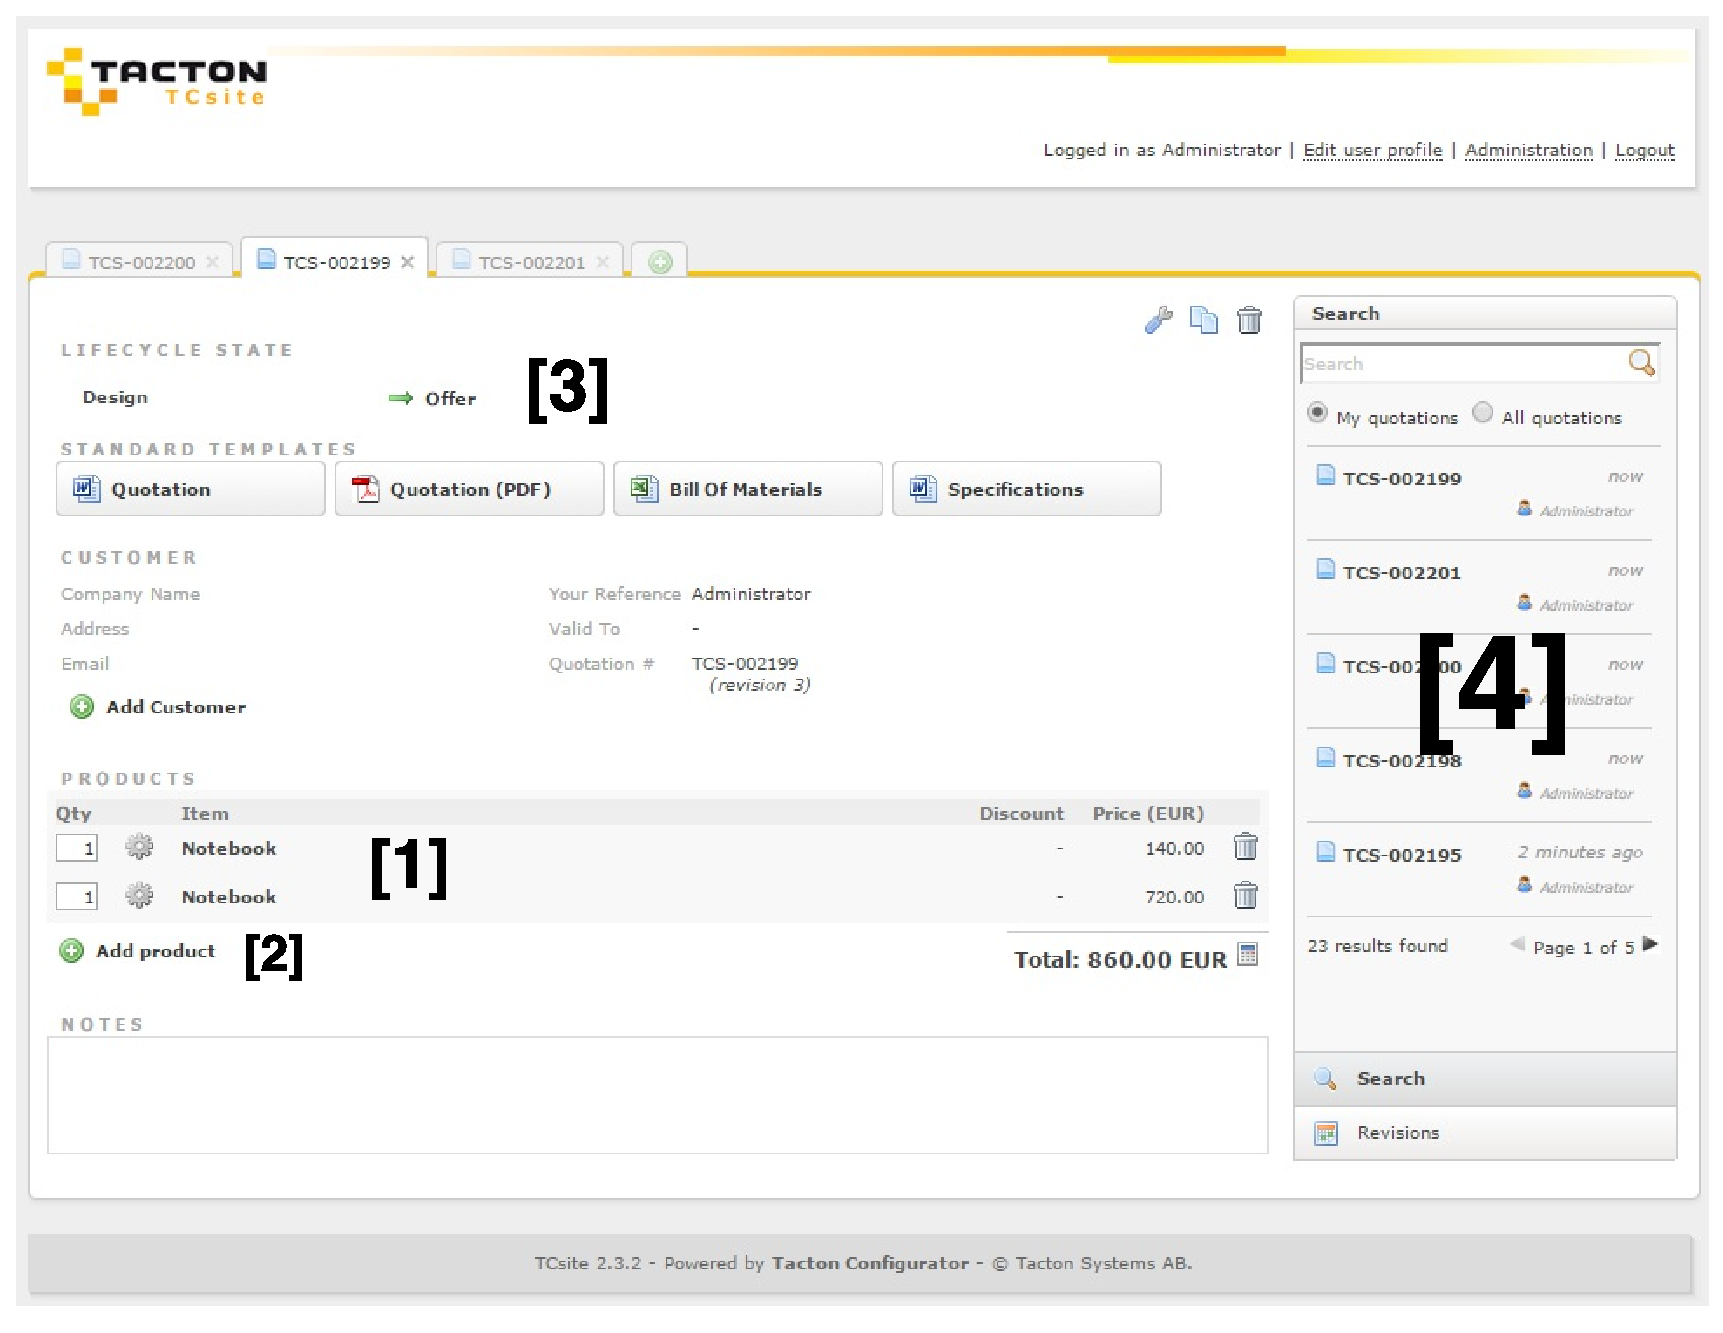
\includegraphics[width=0.95\linewidth]{Abbildungen/tcsiteQuotationNumbered.pdf}
	\captionof{figure}[Quotation-View von TCsite]{Quotation-View von TCsite}
	\label{fig:tcsiteQuotationNumbered}
\end{minipage}
\vspace{1em}

Der Konfigurationsprozess wird über die Schaltfläche 'Add Product' gestartet (siehe [2]). Daraufhin wählt der Anwender das gewünschte Produkt aus einer Liste aus. Im Anschluss erfolgt der Übergang zum Configuration-Modul (Erklärung folgt im nächsten Abschnitt) \citep{tactonTCsiteReferenceManual}.

Eine Quotation hat weiterhin einen Lebenszyklus, welcher unter 'Lifecycle State' dargestellt wird (siehe [3]). Das Angebot befindet sich zu jedem Zeitpunkt in einem bestimmten Zustand, welche über den Administrationsbereich verwaltet werden. Die Zustandsabfolge definiert den sogenannten \emph{Workflow}. Zustände unterscheiden sich in der Sichtbarkeit für verschiedene Nutzergruppen und deren Editierbarkeit. Beispielsweise kann sich eine Quotation in den Zuständen \glqq Design\grqq{} oder \glqq Offered\grqq{} befinden. In letzterem Zustand ist sie nicht mehr änderbar, damit keine Inkonsistenz zum herausgegebenen Angebot entstehen kann \citep{tactonTCsiteReferenceManual}.

Die Box auf der rechten Seite stellt den Index aller Quotations dar (siehe [4]). Unter dem Suchfeld ist einstellbar, ob nur die Quotations des eingeloggten Nutzers gezeigt werden, oder ob nutzerübergreifend gelistet werden sollen. Wie im Administrationsbereich erwähnt, agieren auch externe Systeme als Nutzer, nämlich als Integrationsuser. Auch Quotations, die von dieser Nutzergruppe stammen, werden hier gelistet \citep{tactonTCsiteReferenceManual}.

\subsubsection*{Configuration}
Das Configuration-Modul realisiert den C-Teil des CPQ-Prozesses -- die Konfiguration. Es rendert die Konfigurationsoberfläche und verwaltet die mit der Konfiguration im Zusammenhang stehenden Objekte \citep{tactonTCsiteDevelopmentManual}. Die  technischen Verarbeitungsschritte des Konfigurationsprozesses geschehen jedoch im TCserver. Somit ist die Konfiguration als Client-Server Architektur implementiert. Das Configuration-Modul besitzt Serviceklassen, die die Kommunikation mit der Konfigurationsengine abstrahieren \citep{tactonTCsiteApiDocu}. Ansonsten ist der TCserver nicht unmittelbar ansprechbar.

\subsubsection{Konfigurationsprozess}
\label{TCsiteKonfigurationsprozess}

Abbildung \ref{fig:tcsiteTCserverCommunication} veranschaulicht die Kommunikation zwischen TCsite und TCserver während des Konfigurationsprozesses. Das Configuration-Modul führt wiederholt zustandslose Aufrufe (\emph{configure}) der Konfigurationsengine durch, welche jeweils eine Antwort produzieren (\emph{result}) \citep{tactonTCsiteDevelopmentManual}. Dabei weichen \emph{configure} und \emph{result} semantisch von den Definitionen der Konfigurationsaufgabe und -lösung aus Kapitel \ref{begriffsuberblick} ab.

Um diese Abweichung zu verstehen, muss rekapituliert werden, dass interaktive Konfiguratoren einen Mechanismus zum Merken des Konfigurationszustands besitzen (siehe Kapitel \ref{begriffsuberblick}). Ein Konfigurationszustand beinhaltet bei Tacton, welche Eingabeparameter in welchem Step gewählt wurden. Oben wurde festgestellt, dass die Aufrufe zustandslos sind. Also wird kein serverseitiger Kontext aufgebaut, der den Konfigurationszustand enthält. Die Alternative ist die Übertragung des Zustands in jedem Aufruf.

\vspace{1em}
\begin{minipage}{\linewidth}
	\centering
	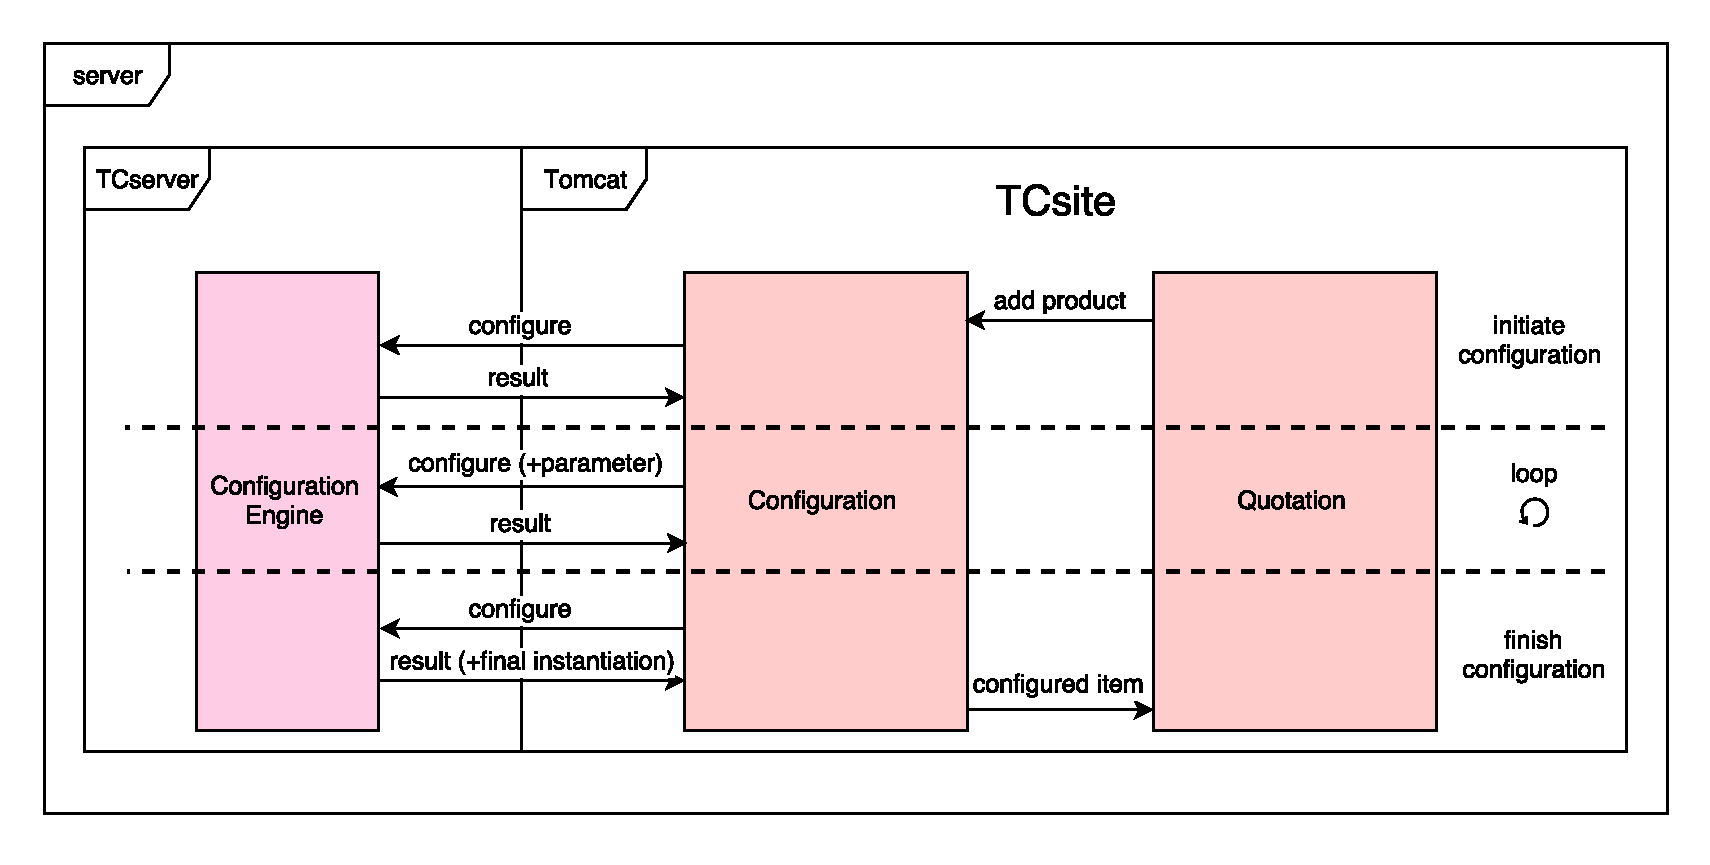
\includegraphics[width=1\linewidth]{Abbildungen/tcsiteTCserverCommunication.pdf}
	\captionof{figure}[Kommunikation zwischen TCsite und TCserver]{Kommunikation zwischen TCsite und TCserver}
	\label{fig:tcsiteTCserverCommunication}
\end{minipage}
\vspace{0.3em}

Demzufolge enthält der configure-Aufruf (1.) das Konfigurationsmodell, (2.) den Konfigurationszustand und fakultativ (3.), den aktuellen Eingabeparameter \citep{tactonTCsiteApiDocu}. Diese Bestandteile werden ab jetzt unter dem Begriff \emph{Konfigurationsengine-Input (KE-Input)} zusammengefasst. Die Antwort (result) beinhaltet primär den neuen Konfigurationszustand. Aus dem result können weiterhin diverse Informationen extrahiert werden -- die finale Instanziierung (Konfigurationslösung), der Endpreis sowie auch die Datengrundlage zum Rendern der Konfigurationsoberfläche \citep{tactonTCsiteApiDocu}. Diese Bestandteile werden ab jetzt unter dem Begriff \emph{Konfigurationsengine-Output (KE-Output)} zusammengefasst.

Der Konfigurationszustand und ein Verweis auf das Konfigurationsmodell, auf dass sich der Konfigurationszustand bezieht, werden in der Klasse \emph{Configurable} zusammengefasst und persistiert. Das \emph{QuotationItem} (vorgestellt in Kapitel  \ref{TCsiteArchitektur}) steht in einer 1-zu-1 Beziehung mit einem \emph{Configurable}.

Die Kommunikation läuft in drei Phasen ab (siehe Abbildung \ref{fig:tcsiteTCserverCommunication}):
\begin{enumerate}
\item[\textbf{initiate configuration}:]Der erste KE-Input beinhaltet noch keinen Eingabeparameter. Er dient dem initialen Aufbau der Konfigurationsoberfläche entsprechend der festgelegten Execution-Struktur im Konfigurationsmodell. Der Konfigurationsprozess startet immer in Step 1. Die Steps müssen in der vordefinierten Reihenfolge abgearbeitet werden.
\item[\textbf{loop}:] Nach jeder Wahl einer Option wird die Konfigurationsengine mit dem Eingabeparameter aufgerufen und daraufhin die Oberfläche neu gerendert. Die Oberfläche spiegelt dabei jeweils den aktuellen Konfigurationszustand wieder, d.h. die bisher gewählten Optionen werden hervorgehoben.
\item[\textbf{finish configuration}:] Wird die Konfiguration im letzten Step vom Anwender abgeschlossen, erfolgt ein finaler Aufruf der Konfigurationsengine. Aus dem KE-Output werden die finale Instanziierung (Konfigurationslösung), der Endpreis, etc. extrahiert \citep{tactonTCsiteDevelopmentManual}.
\end{enumerate}

\vspace{1em}
\begin{minipage}{\linewidth}
	\centering
	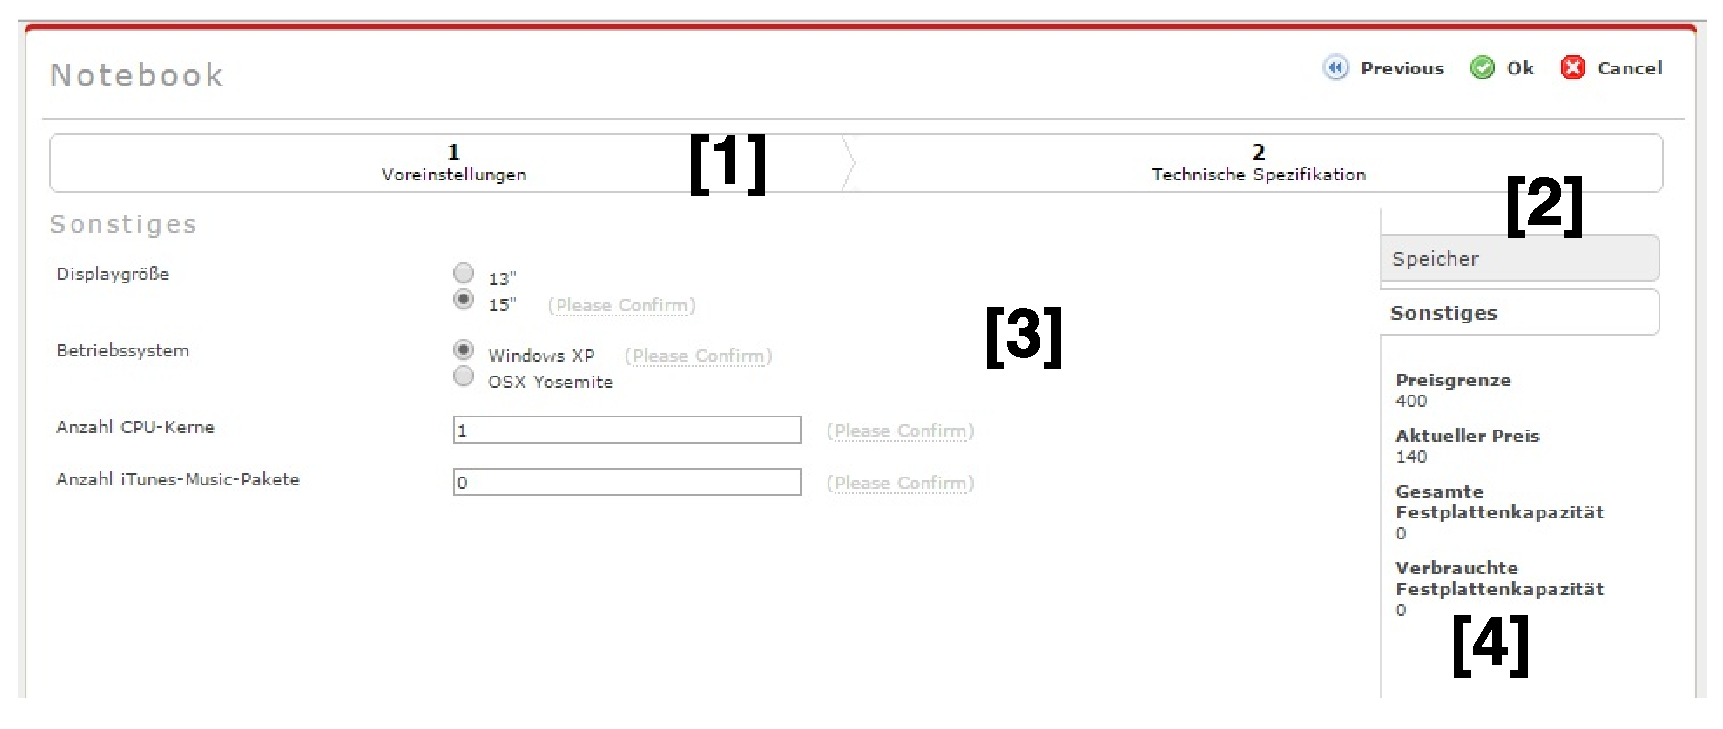
\includegraphics[width=1\linewidth]{Abbildungen/tcsiteConfigurationNumbered.pdf}
	\captionof{figure}[Configuration-View in TCsite der exemplarischen Notebook-Konfiguration]{Configuration-View in TCsite der exemplarischen Notebook-Konfiguration}
	\label{fig:tcsiteConfigurationNumbered}
\end{minipage}
\vspace{0.3em}

Der Konfigurationsprozess in TCsite wird anhand der exemplarischen Notebook-Konfiguration veranschaulicht. Abbildung \ref{fig:tcsiteConfigurationNumbered} zeigt die Konfigurationsoberfläche in TCsite. Das Beispiel befindet sich im zweiten Step. Mittels [1] wird zwischen den Steps gewechselt. [2] erlaubt die Navigation durch die Top-Level-Groups des aktuellen Steps. [3] stellt die Felder der aktuellen Top-Level-Group dar. Anhang \ref{app:tcSiteConfigurationOptionalGroups} zeigt anhand der 'Speicher'-Gruppe die Darstellung der Unterteilung in weitere Gruppen. Außerdem wird unter [4] noch eine zusätzliche Top-Level-Group angezeigt -- die sogenannte \emph{Info-Group}. Sie wird im Konfigurationsmodell durch die Bezeichnung \glqq Info\grqq{} ausgezeichnet und parallel zur gerade aktiven Top-Level-Group im jeweiligen Step dargestellt.

\vspace{1em}
\begin{minipage}{\linewidth}
	\centering
	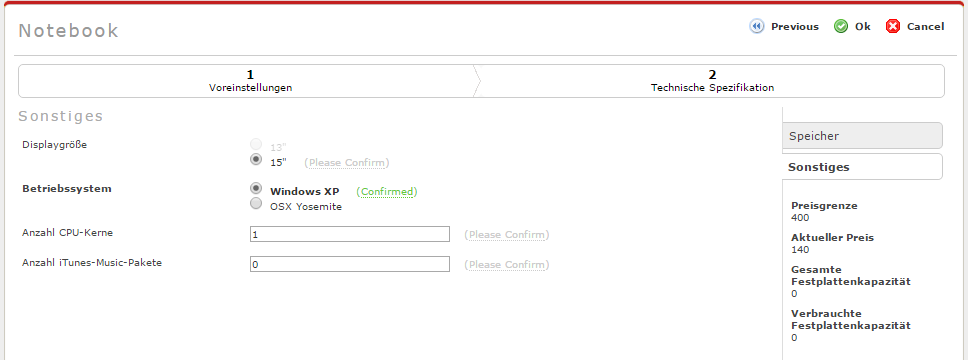
\includegraphics[width=1\linewidth]{Abbildungen/tcsiteConfigurationChoice.PNG}
	\captionof{figure}[Configuration-View in TCsite der exemplarischen Notebook-Konfiguration nach Anwenderwahl]{Configuration-View in TCsite der exemplarischen Notebook-Konfiguration nach Anwenderwahl}
	\label{fig:tcsiteConfigurationChoice}
\end{minipage}
\vspace{0.3em}

Es fällt auf, dass bereits Optionen gewählt sind - obwohl der Anwender noch gar nichts entschieden hat. Offensichtlich hat die Konfigurationsengine initial \emph{Default-Values} gesetzt. Sie sind durch den grauen 'Please Confirm'-Hinweis gekennzeichnet.

Abbildung \ref{fig:tcsiteConfigurationChoice} zeigt die Konfigurationsoberfläche, nachdem der Anwender eine Option gewählt hat (Parameter: 'OS.type', Value: 'Windows XP'). Die gewählte Option wird \emph{unverhandelbar}. Dies wird gekennzeichnet durch das grüne 'Confirmed'. Außerdem wird überprüft, wie die gewählte Option die anderen verfügbaren Optionen beeinflusst. Was bei der Auswahl zu einem Konflikt führen würde, wird ausgegraut. Gleichzeitig ändert die Konfigurationsengine ihre initial selbstgewählten Werte so, dass der aktuelle Konfigurationszustand konsistent ist. Werte, die nicht vom Anwender gesetzt wurden, sind also \emph{verhandelbar}. Die Konfigurationsengine sorgt folglich immer für einen konfliktfreien Zustand. Durch einen Klick auf 'Confirm' bzw. 'Please Confirm' können Optionen zwischen verhandelbar und unverhandelbar gewechselt werden.

\vspace{1em}
\begin{minipage}{\linewidth}
	\centering
	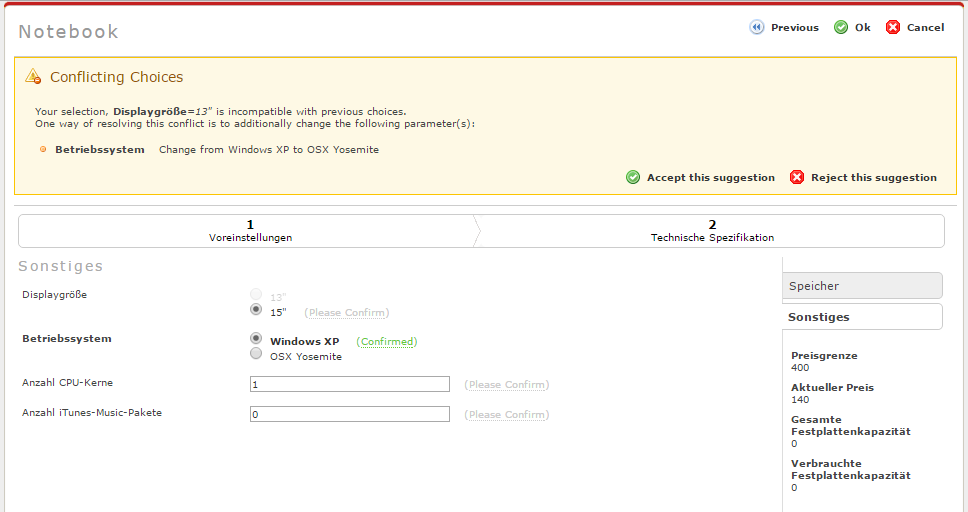
\includegraphics[width=1\linewidth]{Abbildungen/tcsiteConfigurationConflict.PNG}
	\captionof{figure}[Configuration-View in TCsite während einer Konfliktsituation]{Configuration-View in TCsite während einer Konfliktsituation}
	\label{fig:tcsiteConfigurationConflict}
\end{minipage}
\vspace{0.3em}

Ausgegraute Optionen sind dennoch wählbar. Abbildung \ref{fig:tcsiteConfigurationConflict} zeigt die Konfigurationsoberfläche nach einem Klick auf die Displaygröße '13'. Offensichtlich ist '15' jedoch noch immer die aktive Option. Gleichzeitig wird am oberen Ende eine Konflikthinweis angezeigt. Die Konfigurationsengine weist darauf hin, dass Optionen im Widerspruch stehen und schlägt eine Konfliktlösung vor. Diese kann angenommen oder abgelehnt werden. Im letzteren Fall bleibt die Konfiguration einfach in dem Zustand vor der Wahl der konfliktverursachenden Option. Auch die Eingabe von Werten in ein Textfeld kann zu Konflikten führen. Beispielsweise dann, wenn diese außerhalb der Domain des Parameters liegen oder im Widerspruch mit einer anderen Wahl stehen. 

Wird der Konfigurationsprozess über die Schaltfläche 'Ok' beendet, kehrt TCsite zum Quotation-Modul zurück. Dort erscheint die Variante in der Liste der QuotationItems.

\subsubsection{Erweiterbarkeit}
\label{TCsiteErweiterbarkeit}

Zur Erweiterung der Funktionalität bietet TCsite ein Pluginkonzept, welches Abbildung \ref{fig:tcsiteLowLevelExtensions} visualisiert. Neben den oben diskutierten Verantwortlichkeiten definieren die Plattform und die Module sogenannte \emph{Extensionpoints} \citep{tactonTCsiteApiDocu}. Extensionpoints sind das, was in anderen Erweiterungskonzepten als Events bezeichnet wird -- Ereignisse im Kontrollfluss der Geschäftsprozesse. Plugins können Methoden bereitstellen, die an den entsprechenden Ereignisstellen aufgerufen werden \citep{tactonTCsiteDevelopmentManual}.

\vspace{1em}
\begin{minipage}{\linewidth}
	\centering
	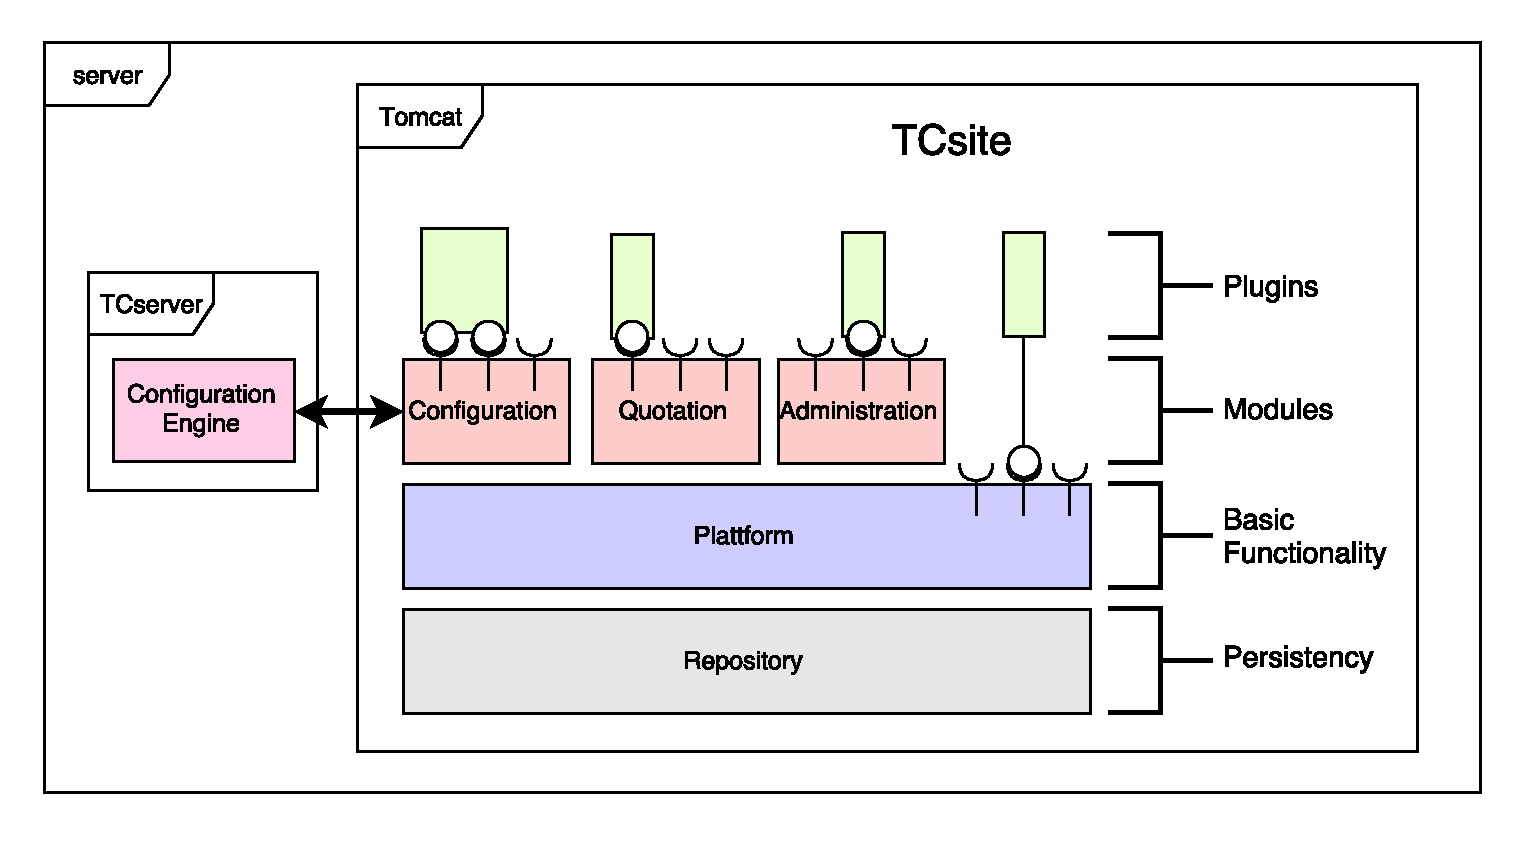
\includegraphics[width=0.8\linewidth]{Abbildungen/tcsiteLowLevelExtensions.pdf}
	\captionof{figure}[TCsite Pluginkonzept]{TCsite Pluginkonzept}
	\label{fig:tcsiteLowLevelExtensions}
\end{minipage}
\vspace{0.3em}

Jedes Plugin hat Zugriff auf das Repository, die Plattform und das Modul, zu dem es gehört. Die Plattform stellt außerdem ein paar spezielle Erweiterungspunkte bereit. Sie erlaubt unter anderem die Definition von \emph{Webcontrollern}. Das sind Methoden, die auf HTTP-Requests an bestimmte URIs innerhalb des TCsite-Addressraums reagieren, diese verarbeiten und mit HTTP-Nachrichten beantworten.

\subsubsection*{Zusammenfassung}
Der Produktkatalog von TCsite besteht nicht aus explizit ausdefinierten Varianten, sondern Produkten mit Konfigurationsmodellen. Erst innerhalb einer \emph{Quotation} werden kundenspezifische Varianten durch einen Konfigurationsprozess generiert, welche als \emph{QuotationItems} bezeichnet werden. Der Konfigurationsprozess ist die Führung des Anwenders durch die in einem Konfigurationsmodell definierte \emph{Execution}, bei dem in jedem Step Optionen gewählt und Eingaben getätigt werden.

Der Konfigurationsprozess passiert im Configuration-Modul. Technisch betrachtet werden dabei \emph{KE-Inputs} verarbeitet, die mit \emph{KE-Outputs} beantwortet werden. Ein KE-Input besteht aus dem Konfigurationsmodell, dessen Konfigurationszustand und (fakultativ) einem Eingabeparameter. Der Konfigurationszustand beinhaltet die Menge aller bisherigen Eingabeparameter. Das \emph{Configurable} erlaubt den Zugriff auf das Konfigurationsmodell und den Konfigurationszustand eine Konfiguration. Der Eingabeparameter resultiert aus den Nutzerinteraktionen mit der Konfigurationsoberfläche. Die Konfigurationsoberfläche wird aus den Daten des \emph{KE-Outputs} erstellt.

\subsection{Zwischenfazit}
\label{TCsiteFazit}

Die Daten aus dem KE-Output können auch einem externen System zum Aufbau einer Konfigurationsoberfläche zur Verfügung gestellt werden. Über die Oberfläche wählt der Anwender Optionen und tätigt Eingaben, woraufhin die Eingabeparameter an TCsite zurückgegeben werden. Dort wird in Verbindung mit dem entsprechenden \emph{Configurable} ein KE-Input definiert. Über den KE-Output kann die Konfigurationsoberfläche im externen System wiederum aktualisiert werden und der Prozess wiederholt sich. Die für diesen Vorgang relevanten Informationen müssen nur irgendwie zwischen dem externen System und TCsite transportiert werden.

Das Pluginkonzept erlaubt die Definition von Webcontrollern. Die in Kapitel \ref{TCsiteErweiterbarkeit} vorgestellte Definition eines Webcontrollers entspricht dem  Umsetzungswerkzeug von REST, welches im Fazit des Kapitels \ref{REST} genannt wurde. Dadurch ist es möglich, einen Webservice zu implementieren, der eine Schnittstelle für externe Konfigurationsoberflächen bereitstellt.

Potentieller Client dieses Services ist jedes System, welches HTTP nutzen kann. Das trifft auf jede Webanwendung zu. eShop-Systeme für den Endverbrauchermarkt sind per se Webanwendungen. Somit können technische Bedingungen an das eShop-System für das Integrationsszenario formuliert werden: (1) Das System muss modifizierbar sein, (2) die Modifizierung muss einen Webservice in einer Client-Server Architektur nutzen können und (3) die Verwaltung von Varianten muss integraler Bestandteil des Systems sein.

Jedes Shopsystem, für welches auf Grundlage dieser Bedingungen eine Daten- und Workflowschnittstelle entwickelt werden kann, kommt für das Integrationsszenario in Frage. Ein interner Evaluierungsprozess der Lino GmbH, bei dem zusätzlich ökonomische Faktoren bewertet wurden, hat zur Favorisierung von \emph{Shopware} für die weitere Entwicklungsarbeit geführt.

\section{Shopsystem}
\label{Shopsystem}

Shopware wird von der shopware AG in Schöppingen entwickelt. Das eShop-System ist aus einer Individuallösung gewachsen, welche 2003 von den heutigen Geschäftsführern entwickelt wurde. Infolgedessen wurde das Unternehmen 2008 als Vertriebsgesellschaft für die Software gegründet. Aktuell liegt die fünfte Version vor. Shopware wird in einem Dual-License Modell vertrieben. Die Community-Edition wird unter der \citeauthor{gnuAGPLv3} Open-Source Lizenz AGPLv3 angeboten. Außerdem existieren drei kommerzielle Versionen \citep{shopwareUnternehmen}.

Im Folgenden wird Shopware einer technischen Analyse unterzogen. Darauf aufbauend wird die Erweiterbarkeit des Systems besprochen. Anschließend wird diskutiert, wie die Produktkonfiguration in der Standardinstallation technisch realisiert wird. Daraus kann eine Abgrenzung zum Tacton Produktkonfigurator gewonnen und gleichzeitig dessen Integration motiviert werden. Die abschließende Betrachtung der Konfiguration im Einkaufsprozess liefert Ansatzpunkte für das Integrationskonzept.

\subsection{Architektur}
\label{shopwareArchitektur}
Shopware basiert auf der Programmiersprache PHP und verwendet eine relationale MySQL Datenbank. Grundlage des Technologiestacks ist das Zend-Framework, welches in der eigenentwickelten Abwandlung namens \glqq Enlight\grqq{} vorliegt \citep{shopware5Docs}.

Abbildung \ref{fig:shopwareMVC} zeigt einen Überblick über die Shopware-Architektur, welche im Folgenden erklärt wird. Eine mit Beispielen angereicherte Variante dieser Abbildung ist Anhang \ref{fig:shopwareMVCLong} zu entnehmen.

Shopware implementiert das Architekturmuster \emph{\ac{MVC}}. Das \emph{Model} definiert die Datenstrukturen des Systems (z.B. Artikel, Kategorien, Bestellungen, etc.). \emph{Doctrine} wird für die \ac{ORM} verwendet. Dadurch wird eine Abstraktionsschicht über der Datenbank aufgebaut \citep{shopware5Docs}. Das Framework ermöglicht die zentrale Definition der Datenbankstruktur in PHP und einen objektorientierten Datenzugriff \citep{shopware4Docs}.

\vspace{1em}
\begin{minipage}{\linewidth}
	\centering
	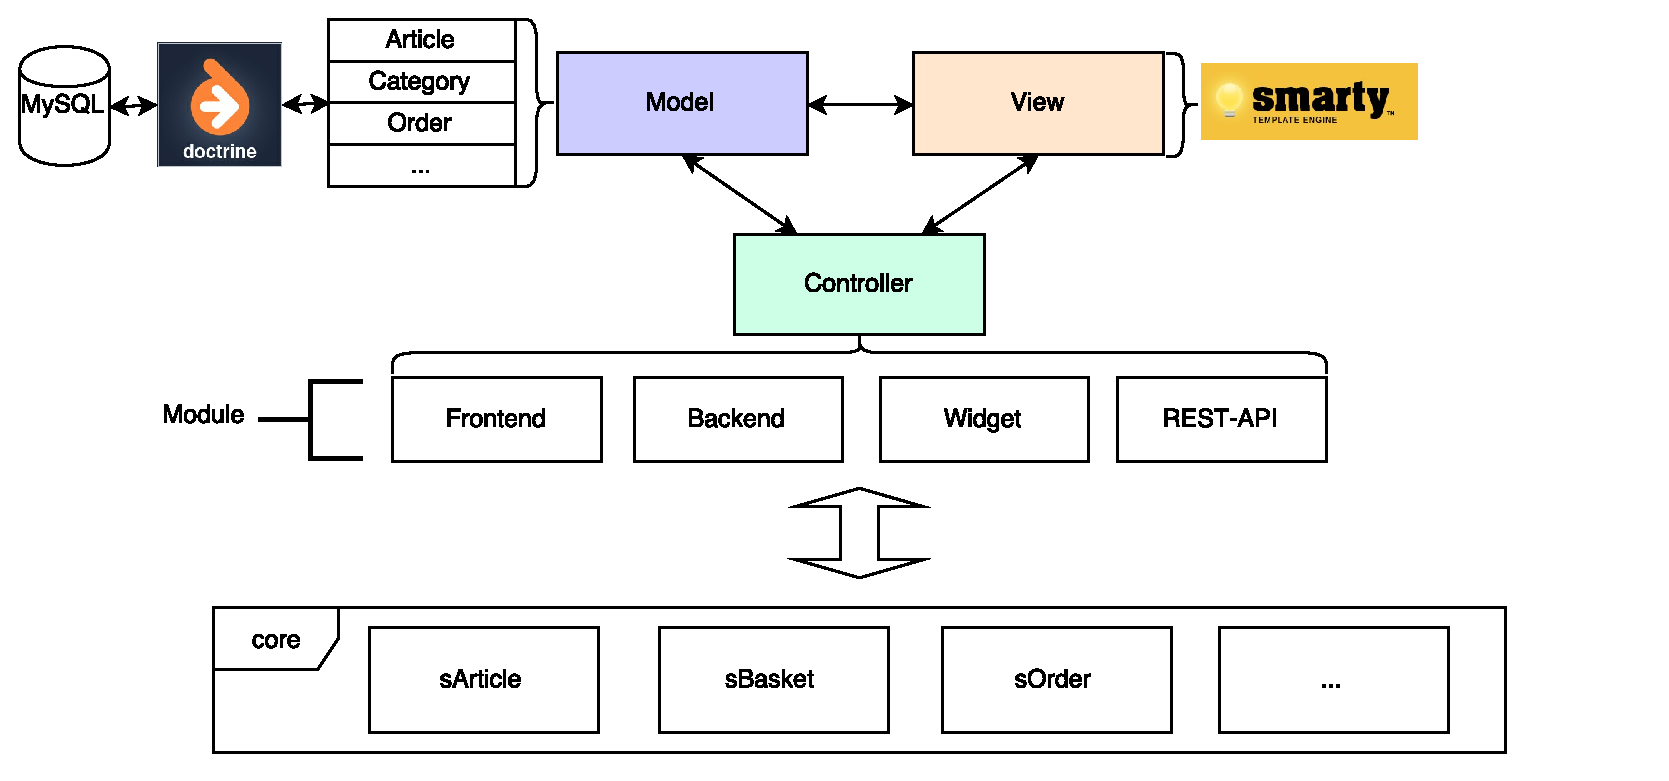
\includegraphics[width=1\linewidth]{Abbildungen/shopwareMVCShort.pdf}
	\captionof{figure}[High-Level-Architektur von Shopware]{High-Level-Architektur von Shopware}
	\label{fig:shopwareMVC}
\end{minipage}
\vspace{0.3em}

Die \emph{View} nutzt die Templating-Engine \emph{Smarty}. Sie erweitert die HTML-Syntax um spezielle \emph{Smarty-Tags}. Diese ermöglichen unter anderem die Definition von Variablen zur Darstellung von Daten aus dem Model. Außerdem können über Smarty-Tags sogenannte \emph{Blöcke} definiert werden. Es handelt sich hierbei um adressierbare Bereiche innerhalb eines Templates, die das Markup strukturieren. Sie spielen eine Rolle für das Erweiterungskonzept \citep{shopware5Docs}.

\emph{Controller} sind Klassen, die HTTP-Requests entgegennehmen und eine Präsentation der Antwort durch Vermittlung zwischen Model und View entwickeln. Sie besitzen Methoden, welche als \emph{Actions} bezeichnet werden. Diese sind  bestimmten URIs zugeordnet. Controller sind nach Verantwortungsbereichen aufgeteilt. Diese werden als Module bezeichnet und folgendermaßen typisiert \citep{shopware4Docs}:
\begin{compactitem}
\item \textbf{Frontend}-Controller sind für die Storefront zuständig. Das betrifft alle Seiten, die ein Kunde sieht.\vspace{0.3em}

Beispiele: Artikelliste einer bestimmten Kategorie, Detailseite eines Artikels, Warenkorb, Nutzeraccount, etc.
\item \textbf{Widget}-Controller generieren wiederverwendbare Bestandteile der Storefront.\vspace{0.3em}

Beispiel: Liste der meistverkauften Artikel
\item \textbf{Backend}-Controller sind für die Datenverwaltung der Shopadministration zuständig. Sie generieren jedoch keine Einzelseiten wie im Falle der Frontend-Controller. Stattdessen ist der administrative Bereich als Single-Page-Application mittels des Javascript-Frameworks \emph{Ext JS} implementiert. Dieses stellt eine Menge an Steuerelementen (z.B. Menüs, Formulare, etc.) zur Verfügung.\vspace{0.3em}

Beispiele: Nutzerverwaltung, Artikelverwaltung, Pluginverwaltung, etc.
\item Für externe Systeme, die mit den Ressourcen von Shopware interagieren möchten, ist eine \textbf{REST-API} implementiert. Ein vollständige Übersicht aller Ressourcenendpunkte ist \citet{shopwareRestApiEndpunkte} zu entnehmen.\vspace{0.3em}

Beispiel: Abrufen des Artikels mit der ID 167.
\end{compactitem}

Der Großteil der Logik ist jedoch nicht in den Actions, sondern den sogenannten \emph{Core}-Klassen implementiert \citep{shopware4Docs}. Beispielsweise wird der Request zum Hinzufügen einer Warenkorbposition zwar vom Checkout-Controller entgegengenommen, die notwendigen Geschäftsprozesse finden aber in der Serviceklasse \emph{sBasket} statt.

\subsection{Erweiterbarkeit}
\label{shopwareErweiterbarkeit}
Der Quellcode der Community-Edition liegt offen. Theoretisch ist eine Erweiterung der Funktionalität über ein direktes Eingreifen in den Shopware-Kern möglich. Der Hersteller sieht jedoch eine Anpassung über Plugins vor. Entsprechend der \ac{MVC}-Architektur wird in \emph{logische Erweiterungen} (betrifft Controller), \emph{Daten-Erweiterungen} (betrifft Model) und \emph{Template-Erweiterungen} (betrifft View) unterschieden \citep{shopware5Docs}.

\subsubsection*{Logische Erweiterungen}
Logische Erweiterungen werden über \emph{Events} und \emph{Hooks} realisiert. Events sind \glqq definierte Ereignisse, die im Workflow des Shops auftreten\grqq{} \citep{shopware4Docs}. Plugins können Code registrieren, welcher an den Ereignispunkten ausgeführt wird. Steht kein Event für die geplante Modifikation zur Verfügung, kann Plugin-Code über das Hooksystem unmittelbar auf Funktionen des Shopware-Kerns registriert werden \citep{shopware5Docs}. Damit ist das Erweiterungskonzept flexibler als das von TCsite. Im Folgenden werden die Konzepte detaillierter vorgestellt.

Events werden in \emph{Controller-Events} und \emph{Notify-Events} unterschieden \citep{shopware4Docs}. Controller-Events sind an den \emph{Dispatch}-Vorgang gekoppelt. Der shopware-Entwickler \citet{noegel15Diaspatch} definiert Dispatching als einen Prozess, bei dem das Request-Objekt gehandhabt, daraus das relevante Modul, der Controller und die Action extrahiert, der entsprechende Controller instanziiert und dieser zur Behandlung des Requests gebracht wird. Leitet ein Controller den Request zu einem anderen Controller weiter, wiederholt sich dieser Vorgang. Plugins können Code registrieren, der vor (\emph{PreDispatch}) oder nach dem Dispatching (\emph{PostDispatch}) ausgeführt werden soll. Außerdem können sie den Dispatch-Prozess auf eigene Funktionen umleiten und so ganze Controller-Methoden ersetzen. Notify-Events entsprechen hingegen den in Kapitel \ref{TCsiteErweiterbarkeit} erwähnten Extension-Points von TCsite. Sie finden beispielsweise in den Core-Klassen Verwendung. So kann abseits der Controller in den Programmablauf eingegriffen werden \citep{shopware4Docs}.

Hooks bieten einen generischeren Ansatz. Events sind auf den Dispatchprozess und alle sonstigen Punkte beschränkt, an denen ein Shopware-Entwickler den Eingriff eines Plugins vorgedacht hat. Das Hooksystem bezeichnet die Möglichkeit, jede Public- und Protected-Funktion von Shopware zu erweitern. Hooks erlauben die Modifizierung der Eingangsparameter und Rückgabewerte der Originalfunktion sowie deren komplette Ersetzung \citep{noegel15Hooks}.

\subsubsection*{Daten-Erweiterungen}
Im Gegensatz zu TCsite erlaubt Shopware die Erstellung und Modifizierung von Datenbanktabellen. Sollen bestehende Datenmodelle nur um bestimmte Eigenschaften ergänzt werden, kommt das \emph{Attributsystem} in Frage. Gewisse Shopware-Entitäten (z.B. \emph{s\_user} für Shopkunden) haben Attributtabellen (z.B. \emph{s\_user\_attributes}) in einer 1-zu-1 Beziehung zugeordnet. Plugins können diesen Tabellen beliebige Spalten hinzufügen (z.B. die Lieblingsfarbe des Kunden) \citep{shopware5Docs}.

\subsubsection*{Template-Erweiterungen}
Die View bietet Erweiterungspunkte über das Smarty-Block-System. Die Blöcke können durch eigenen Templatecode ersetzt oder erweitert werden. Weiterführend sind so eigene CSS- und Javascriptdateien im Seitenkopf einbindbar. Folglich kann mittels Template-Erweiterungen auch clientseitige Logik realisiert werden.

Abschließend wird bemerkt, dass Oberflächenerweiterungen im administrativen Bereich nicht durch Smarty realisiert werden, sondern durch das dort eingesetzte Framework Ext JS. Dies wird nicht in der offiziellen Dokumentation erwähnt. Stattdessen weisen die Orientierungsbeispiele für Backenderweiterungen implizit darauf hin (siehe \citet{shopwareBackendPluginExamples}). Ext JS-Erweiterungen sind ein komplexer Sachverhalt und werden in dieser Arbeit nicht weiter behandelt.

\subsection{Konfiguration}
\label{shopwareKonfiguration}
Shopware behauptet in der der offiziellen Funktionsübersicht, bereits in der Standardinstallation einen Konfigurator zu besitzen \citep{shopware5Funktionsuebersicht}. Im Folgenden wird dessen Implementierung sowie Integration in den Einkaufsvorgang analysiert.

\subsubsection{Technische Analyse}
\label{shopwareKonfigurationAnalyse}
Ein Artikel, den ein Kunde kaufen kann, wird über den entsprechenden Menüpunkt im Backend angelegt (siehe Anhang \ref{app:shopwareBackendArtikel}). Über das Userinterface kann dieser als \emph{Varianten-Artikel} gekennzeichnet werden. Dadurch wird der Variantenreiter aktiviert, unter dem der Administrator alle Varianten des Artikels festlegt.

Dazu werden sogenannte \emph{Gruppen}\footnote{Nicht zu verwechseln mit den Gruppen des TCsite-Modells, siehe Kapitel \ref{Execution}.} (z.B. 'Storage') angelegt, die wiederum \emph{Optionen}\footnote{Ebenfalls nicht zu verwechseln mit den Optionen des TCsite-Modells.} (z.B. 'HDD' oder 'SSD') besitzen. Das ist äquivalent zu den Begriffen \emph{Parameter} und \emph{Domain} in der Execution des Tacton-Konfigurationsmodells, vorgestellt in Kapitel \ref{Execution}. Es werden also die Wahlmöglichkeiten des Anwenders definiert, jedoch ohne Konfigurationswissen. Die Gruppen und Optionen werden separat in der Datenbank gespeichert und sind Artikelübergreifend verwendbar. Über den Button \glqq Varianten generieren\grqq{} (siehe Anhang \ref{app:shopwareBackendArtikelVarianten}) werden alle Varianten explizit in der Datenbank angelegt, die sich aus der Kombination der Optionen ergeben. Übertragen auf das Notebook-Beispiel ergibt das folgende Rechnung:

\begin{addmargin}[40pt]{0pt} 
$\;\;\;3_{Massenspeicher1}\\\cdot\;3_{Massenspeicher2}\\\cdot\;2_{Arbeitsspeicher}\\\cdot\;2_{Displaygr"o"se}\\\cdot\;2_{Betriebssystem}\\\cdot\;4_{Anzahl\;CPU-Kerne}\\\cdot\;99_{Anzahl\;iTunes-Music-Pakete}\\= 28512\;Varianten$
\end{addmargin}

Damit passiert das, was durch das Konfigurationsmodell laut Kapitel \ref{begriffsuberblick} verhindert werden soll -- das explizite Definieren und Abspeichern aller Varianten. Es gibt keine Constraints. Dementsprechend muss der Administrator händisch alle inkorrekten Varianten löschen und die Preise der korrekten Varianten nachtragen.

Die in Kapitel \ref{begriffsuberblick} vorgestellte Konfigurationsdefinition von \citet{sabin98} fordert Constraints. Somit stellt Shopware keinen Konfigurationsprozess bereit, sondern die Selektion einer explizit definierten Variante aus einer Datenbank entsprechend der gewählten Optionen des Anwenders.

\subsubsection{Einkaufsvorgang}
\label{shopwareEinkaufsvorgang}
Ausgehend von dieser Analyse ist der Einkaufsvorgang eines Varianten-Artikels unter Berücksichtigung der technischen Prozesse als Aktivitätsdiagramm in Abbildung \ref{fig:shopwareKonfigurationFlussdiagramm} darstellbar.

\vspace{1em}
\begin{minipage}{\linewidth}
	\centering
	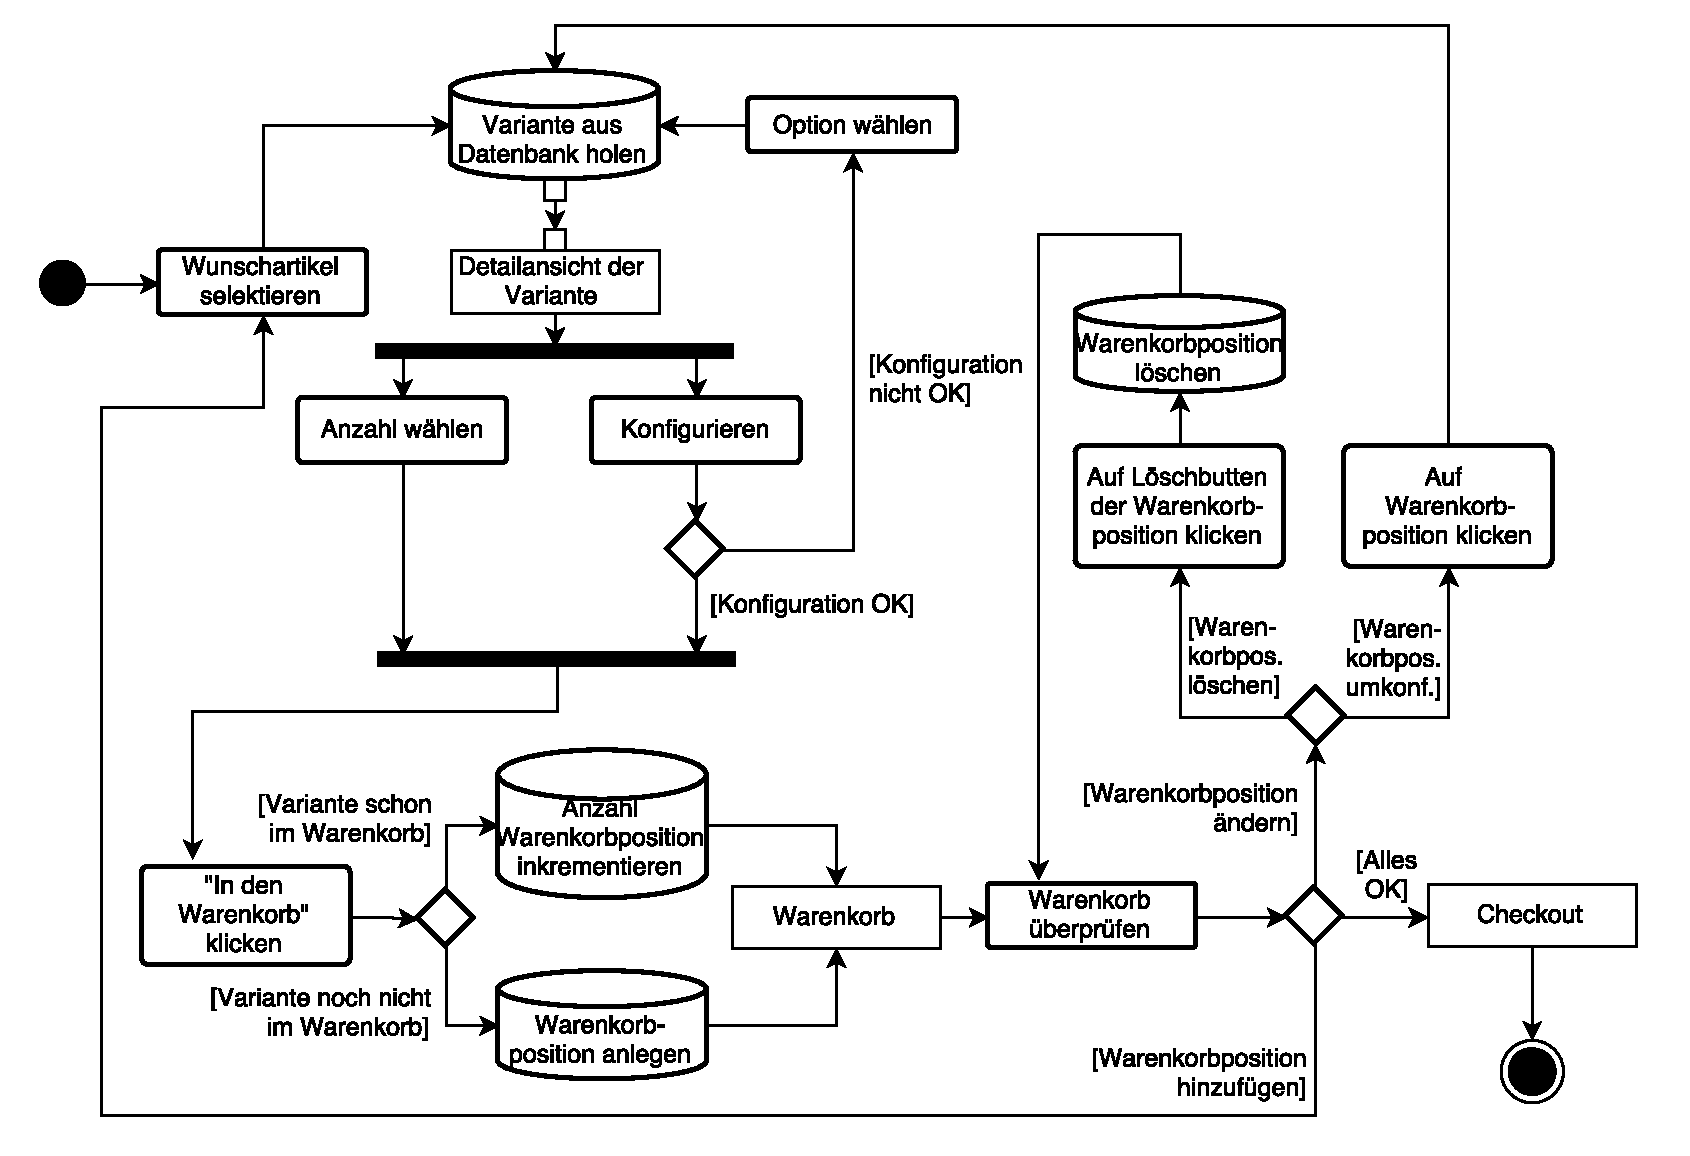
\includegraphics[width=1\linewidth]{Abbildungen/shopwareKonfigurationFlussdiagramm.pdf}
	\captionof{figure}[Aktivitätsdiagramm des Einkaufsvorgangs eines Varianten-Artikels in Shopware]{Aktivitätsdiagramm des Einkaufsvorgangs eines Varianten-Artikels in Shopware}
	\label{fig:shopwareKonfigurationFlussdiagramm}
\end{minipage}
\vspace{0.3em}

Mittels der Katalog- oder Suchfunktion wählt der Kunde einen konfigurierbaren Artikel aus - d.h., er wurde im Backend als \emph{Varianten-Artikel} gekennzeichnet. Auf der Detailseite wird die erste Variante des Artikels angezeigt. Dazu muss angemerkt werden, dass im Backend eingestellt wird, welche Variante eine Artikels initial geladen werden soll. Diese Variante wird ab jetzt als \emph{Basisvariante} bezeichnet. Neben beschreibenden Texten und Bildern befindet sich auf der Detailseite die Konfigurationsoberfläche (siehe Anhang \ref{app:shopwareNotebookDetail}). Zu jeder Gruppe wird ein Menü mit den entsprechenden Optionen angezeigt. Die Auswahl einer Option führt zum Reload der Seite mit der aktuellen Variante. Dieser Vorgang wiederholt sich so lange, bis der Artikel den Vorstellungen des Kunden entspricht. Außerdem wird die gewünschte Kaufmenge (Anzahl) eingestellt. Über den \glqq In den Warenkorb\grqq{}-Button wird der Artikel in den Warenkorb gelegt. Ist diese Variante bereits im Warenkorb, wird die Anzahl der entsprechenden Warenkorbposition inkrementiert. Anderenfalls entsteht eine neue Warenkorbposition. An der Bezeichnung der Warenkorbpositionen ist ablesbar, welche Optionskombination jeweils vorliegt (siehe Anhang \ref{app:shopwareNotebookWarenkorb}). Nun überprüft der Kunde den Warenkorb. Möchte er weitere Artikel hinzufügen, beginnt der Prozess mit der Auswahl des Wunschartikels von vorne. Ist der Kunde mit der Konfiguration einer Warenkorbposition noch nicht zufrieden, kann er diese löschen oder ändern. Möchte er sie ändern, kommt er über einen Klick auf die entsprechende Position zur Detailansicht dieser Variante zurück. Nun können andere Optionen gewählt werden. Ein erneuter Klick auf \glqq In den Warenkorb\grqq{} aktualisiert nicht etwa die zugehörige Warenkorbposition, sondern erzeugt einen neue. Die alte Variante verbleibt zusätzlich im Warenkorb. Ist der Nutzer mit allen Positionen im Warenkorb zufrieden, wird der Bestellvorgang über den Checkout-Prozess abgeschlossen.

Dieser Vorgang illustriert den Lebenszyklus einer Variante in Shopware. Er beginnt mit dem Anlegen aller Varianten eines Artikels im Backend. Das ist ein Unterschied zu der Umsetzung in TCsite, welche in Kapitel \ref{TCsiteArchitektur}
 besprochen wurde. Hier beginnt der Lebenszyklus erst mit der Konfiguration.

\section{Fazit}
\label{analyseFazit}
Shopware bietet in der Standardinstallation keine Funktionalität, die der Definition eines Konfigurationsprozesses gerecht wird. Stattdessen wird eine \emph{Variantenselektion} durchgeführt. Da alle Varianten expliziert vordefiniert sind, werden dadurch die in Kapitel \ref{Produktklassifizierung} beschriebenen \ac{ATO}-Produkte abgebildet. Die Analyse in Kapitel \ref{tactonKonfigurationsmodell} hat ergeben, dass das Tacton-Konfigurationsmodell auch \ac{MTO}-Produkte abbilden kann. Eine Integration des Tacton Produktkonfigurators in Shopware würde somit dessen Angebotsspektrum in Bezug auf Produktionskonzepte erweitern.

In Kapitel \ref{shopwareErweiterbarkeit} wurde das Plugin-Konzept von Shopware vorgestellt. Template-Erweiterungen erlauben einen Eingriff in die Oberfläche. Damit ist eine Konfigurationsoberfläche in Shopware darstellbar. Die Analyse des Einkaufsvorgangs von konfigurierbaren Artikeln in Kapitel \ref{shopwareEinkaufsvorgang} impliziert jedoch Änderungen über die reine Integration einer Konfigurationsoberfläche hinaus. Nach dem Konfigurationsprozess absolvieren Varianten weitere Stationen im Einkaufsvorgang. Für die Arbeit bedeutet dies, dass ein Shopware-Plugin zu erstellen ist, welches (1.) eine Konfigurationsoberfläche bereitstellt und (2.) die resultierenden Varianten in den Einkaufsvorgang integriert.

Im Zwischenfazit der TCsite-Analyse (Kapitel \ref{TCsiteFazit}) wurde
geschlussfolgert, dass eine Konfigurationsoberfläche auch in einem externen System umsetzbar ist. Über Webcontroller kann ein Webservice implementiert werden, mit dem die Konfigurationsoberfläche kommuniziert. Webcontroller werden via Plugin definiert. Zusätzlich wurde oben festgestellt, dass das Shopware-Plugin nicht nur eine Konfigurationsoberfläche bereitstellen, sondern auch die resultierenden Varianten in den Einkaufsvorgang integrieren muss. Für die Arbeit bedeutet dies, dass ein TCsite-Plugin zu erstellen ist, welches (1.) eine Schnittstelle für externe Konfigurationsoberflächen anbietet und (2.) alle sonstigen Daten zur Integration einer Variante in den Einkaufsvorgang zur Verfügung stellt. 

Nach diesem Grobkonzept der Verantwortungsbereiche wird in der folgenden Anforderungsanalyse definiert, was die beiden Plugins im Detail leisten müssen.

\chapter{Anforderungsanalyse}
Es ist ein System zu entwickeln, welches die Verbindung zwischen TCsite und Shopware herstellt. Dieses System wird in Abbildung \ref{fig:systemcontext} in eine Beziehung mit den Elementen gebracht, welche aus der Analyse des vorherigen Kapitels hervorgehen. Der Systemkontext stellt die Umgebung dar, der die für die Entwicklung relevanten Aspekte beinhaltet. Was das System hingegen nicht beeinflusst, ist Teil der irrelevanten Umgebung.

In Kapitel \ref{TCsiteArchitektur} wurde erwähnt, dass die Kommunikation mit dem TCserver vom Configuration-Modul abstrahiert wird. Von außen ist also nicht ersichtlich, dass der Konfigurationsprozess durch eine Serveranwendung realisiert wird. TCserver ist also Teil der irrelevanten Umgebung.

Zum Systemkontext gehört TCsite, da es das Configuration-Modul beherbergt. Außerdem verwaltet die Anwendung die Konfigurationsmodelle und -zustände. Weiterhin ist Shopware teil des Kontexts. Dort soll eine Konfigurationsoberfläche zur Verfügung gestellt und die resultierenden Varianten in den Einkausfsvorgang integriert werden. Der Shopkunde und -administrator sind die relevanten Stakeholder von Shopware. Sie werden mit dem Plugin interagieren.
Im Zentrum des Systemkontexts befindet sich das zu entwickelnde System selbst.

\vspace{1em}
\begin{minipage}{\linewidth}
	\centering
	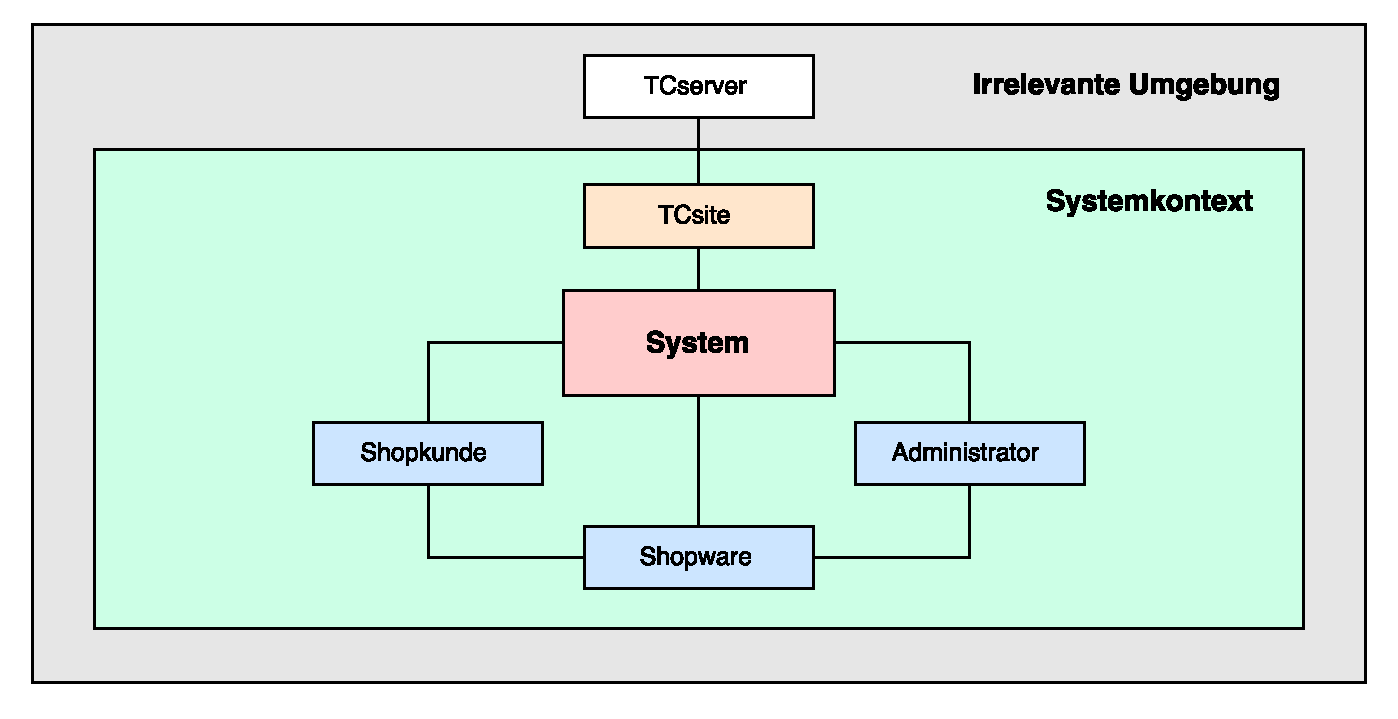
\includegraphics[width=0.8\linewidth]{Abbildungen/systemcontext.pdf}
	\captionof{figure}[Systemkontext]{Systemkontext}
	\label{fig:systemcontext}
\end{minipage}
\vspace{0.3em}

Ausgehend von dem Fazit des vorherigen Kapitels kann das System feingranularer bestimmt werden, wie Abbildung \ref{fig:systemcontextErweitert} darstellt. Im Fazit des vorangegangenen Kapitels wurde beschrieben, dass sowohl für TCsite als auch für Shopware Plugins entwickelt werden müssen. Das TCsite-Plugin stellt eine Schnittstelle als Webservice bereit, welche vom Shopware-Plugin genutzt wird. Darum besteht eine Verbindung zwischen beiden Plugins.

In Kapitel \ref{Webservices} wurde besprochen, dass Webservices nicht direkt von menschlichen Anwendern genutzt werden. Darum steht keiner der Stakeholder in Verbindung zum TCsite-Plugin. Hingegen werden Shopkunden im Frontend und der Administrator im Backend mit dem Shopware-Plugin interagieren.

\vspace{1em}
\begin{minipage}{\linewidth}
	\centering
	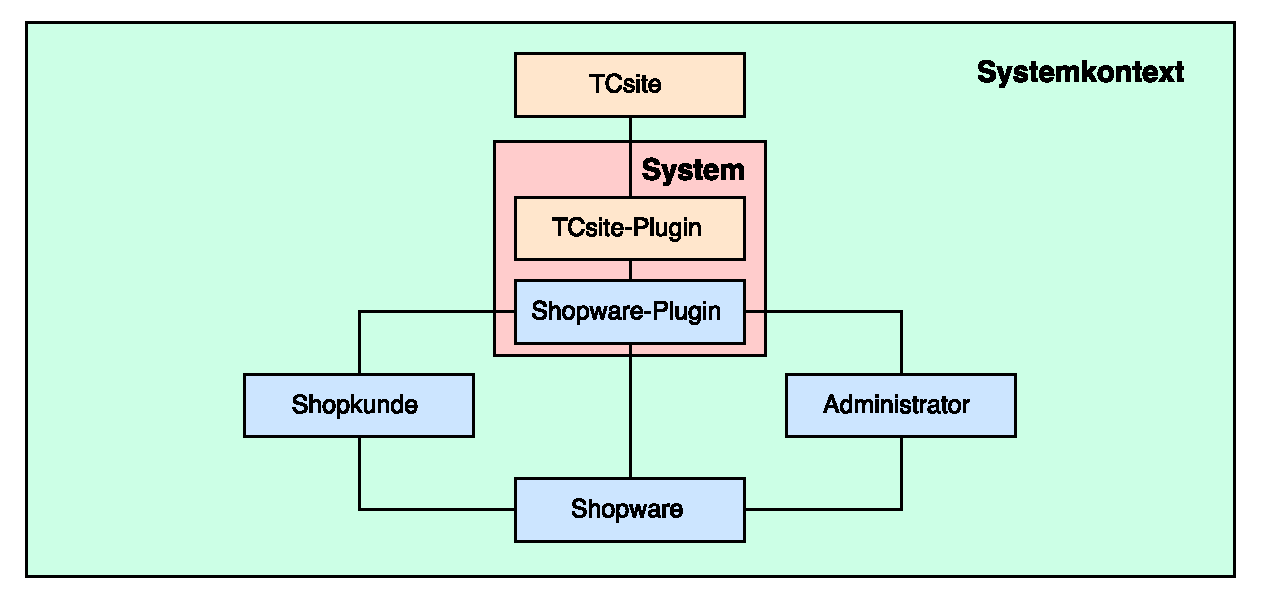
\includegraphics[width=0.8\linewidth]{Abbildungen/systemcontextErweitert.pdf}
	\captionof{figure}[Erweiterter Systemkontext]{Erweiterter Systemkontext}
	\label{fig:systemcontextErweitert}
\end{minipage}
\vspace{0.3em}

Basierend auf den Systemkontext werden nun Anforderungen spezifiziert, die sich auf das System und die Aspekte des Systemkontexts beziehen. Es wird in funktionale und nichtfunktionale Anforderungen unterschieden.

\section{Funktionale Anforderungen}

Funktionale Anforderungen beschreiben das \glqq was\grqq{}, d.h. welche Funktionalitäten und Dienste das System erfüllen soll. Es werden zunächst die funktionalen Anforderungen des Shopware-Plugins vorgestellt. Aus diesen ergibt sich, was das TCsite-Plugin als Webservice liefern muss.

\subsection{Shopware-Plugin}
Die Analyse des Einkaufsvorgangs in Kapitel \ref{shopwareEinkaufsvorgang} hat ergeben, dass die Konfiguration eines Artikels auf dessen Detailseite stattfindet. Daraus ergibt sich folgende Anforderung:
\begin{enumerate}[SW.F01:]\bfseries
\item Das Shopware-Plugin muss auf der Detailseite eine Konfigurationsoberfläche bieten.
\end{enumerate}
Die Funktionalität der Konfigurationsoberfläche kann näher beschrieben werden. Aus der Analyse des Konfigurationsprozesses in TCsite (siehe Kapitel \ref{TCsiteKonfigurationsprozess}) ergibt sich die folgende Anforderung:
\begin{enumerate}[SW.F02:]\bfseries
\item Die Konfigurationsoberfläche muss einen Konfigurationsprozess äquivalent zu TCsite ermöglichen. 
\end{enumerate}
Das beinhaltet: Aktualisierung der Oberfläche nach jeder Wahl des Anwenders; Darstellung von Steps, Toplevel-Groups, optionalen Gruppen, allen Feldtypen; Hervorhebung der verhandelbar/nichtverhandelbar gesetzten Werte; Navigation durch die Execution-Struktur (Steps in vordefinierter Reihenfolge, Toplevel-Groups); Wählen von Optionen, Eingabe von Werten; Wechsel des Optionszustands zwischen verhandelbar/nichtverhandelbar; Konfliktbehebung;

Im Fazit des Kapitels \ref{analyseFazit} wurde festgelegt, dass die aus dem Konfigurationsprozess resultierenden Varianten in den Einkaufsvorgang integriert werden müssen. Die dementsprechende Anforderung lautet:
\begin{enumerate}[SW.F03:]\bfseries
\item Die aus dem Konfigurationsprozess resultierende Variante muss sich in den Einkaufsvorgang integrieren.
\end{enumerate}
Diese Anforderung stellt die Basis der folgenden Anforderungen dar.

Damit eine Variante gekauft werden kann, benötigt sie einen Preis. Dieser wird unter anderem auf der Detailseite angezeigt. Er muss nach jeder Nutzerinteraktion neu berechnet werden. Daraus ergibt sich folgende Anforderung:
\begin{enumerate}[SW.F04:]\bfseries
\item Die Detailseite muss den aktuellen Preis der Variante anzeigen.
\end{enumerate}
Von der Detailseite aus kommt die Variante in den Warenkorb. Die dementsprechende Anforderung lautet:
\begin{enumerate}[SW.F05:]\bfseries
\item Die Detailseite muss das Ablegen der Variante in den Warenkorb ermöglichen.
\end{enumerate}
Dabei müssen Preis und Anzahl entsprechend von der Detailseite übernommen werden..

In Kapitel \ref{TCsiteKonfigurationsprozess} wurde bei der Analyse des Konfigurationsprozesses in TCsite festgestellt, dass diese erst im letzten Step abgeschlossen werden kann. Äquivalent resultiert für das Shopszenario folgende Anforderung, die eine detailliertere Beschreibung der Anforderung SW.F05 darstellt:
\begin{enumerate}[SW.F06:]\bfseries
\item Die Variante muss erst im letzten Step in den Warenkorb legbar sein.
\end{enumerate}
Eine Variante im Warenkorb stellt eine Warenkorbposition dar. Bei unterschiedlichen Varianten im Warenkorb muss der Kunde diese unterscheiden können. Daraus resultiert die Anforderung:
\begin{enumerate}[SW.F07:]\bfseries
\item Warenkorbpositionen müssen eine Beschreibung bieten.
\end{enumerate}
Der Umfang der Beschreibung muss angemessen sein. Bei Konfigurationen mit vielen Parametern kommt eine Aufzählung aller gewählter Optionen also nicht in Frage. Es muss eine \emph{Kurzbeschreibung} geboten werden.

Der in Kapitel \ref{shopwareEinkaufsvorgang} vorgestellte Einkaufsvorgang beinhaltet die Umkonfiguration von Warenkorbposition. Daraus resultiert folgende Anforderung: 
\begin{enumerate}[SW.F08:]\bfseries
\item Warenkorbpositionen müssen umkonfigurierbar sein.
\end{enumerate}
Umkonfiguration wird in dieser Arbeit als Aktualisierung einer Warenkorbposition verstanden. Dadurch ändert sich, welche Variante durch eine Warenkorbposition repräsentiert wird. Somit resultiert implizit, dass eine Umkonfiguration nicht zur Erstellung einer neuen Warenkorbposition führt, wie dies im bisherigen Einkaufsvorgang von Shopware der Fall ist.

Die Umkonfiguration findet auf der Detailseite statt. Die dementsprechende Anforderung lautet: 
\begin{enumerate}[SW.F09:]\bfseries
\item Die Detailseite einer Warenkorbposition muss aufrufbar sein.
\end{enumerate}
Auf der Detailseite soll die Konfiguration jedoch nicht neu beginnen, sondern dem letzten Konfigurationszustand entsprechen. Daraus resultiert die folgende Anforderung:
\begin{enumerate}[SW.F10:]\bfseries
\item Die Detailseite muss dem Konfigurationszustand einer Warenkorbposition entsprechen.
\end{enumerate}
Das beinhaltet den Preis und die Konfigurationsoberfläche.

Im bisherigen Einkaufsvorgang (siehe Kapitel \ref{shopwareEinkaufsvorgang}) wird die Umkonfiguration erst beim erneuten Ablegen der Variante in den Warenkorb registriert. Die dementsprechende Anforderung lautet folgendermaßen:
\begin{enumerate}[SW.F11:]\bfseries
\item Auf der Artikeldetailseite muss die Umkonfiguration einer Warenkorbposition durch einen entsprechenden Button vom Kunden bestätigt werden.
\end{enumerate}
Durch eine Umkonfiguration ist es möglich, dass zwei ursprünglich unterschiedliche Warenkorbpositionen nun die gleiche Variante repräsentieren. Die Warenkorbpositionen sollen jedoch weiterhin separat umkonfigurierbar sein. Daraus resultiert die folgende Anforderung:
\begin{enumerate}[SW.F12:]\bfseries
\item Im Warenkorb muss jede Variante eine eigene Position darstellen.
\end{enumerate}
Beim bisherigen Einkaufsvorgang (siehe Kapitel \ref{shopwareEinkaufsvorgang}) sind Warenkorbpositionen löschbar. Die dementsprechende Anforderung lautet folgendermaßen:
\begin{enumerate}[SW.F13:]\bfseries
\item Im Warenkorb müssen Varianten löschbar sein.
\end{enumerate}
Die nächste Station des Einkaufsvorgangs ist die Bestellung. Daraus resultiert die folgende Anforderung:
\begin{enumerate}[SW.F14:]\bfseries
\item In der Bestellung müssen die Warenkorbpositionen übernommen werden.
\end{enumerate}
Äquivalent zum Warenkorb muss auch in der Bestellbestätigung ersichtlich sein, welche Varianten bestellt wurden (Preis, Anzahl, Kurzbeschreibung, etc.). Dementsprechend lautet die folgende Anforderung:
\begin{enumerate}[SW.F15:]\bfseries
\item In der Bestellbestätigung für den Kunden müssen die Beschreibungen der Warenkorbpositionen übernommen werden.
\end{enumerate}
Bis jetzt wurde unterschlagen, dass auf Übersichtsseiten wie z.B. dem Artikellisting (siehe Anhang \ref{app:shopwareArtikelListing}) bereits Preise verzeichnet werden. Diese stehen vor der Konfiguration aber noch nicht fest. Die dementsprechende Anforderung lautet:
\begin{enumerate}[SW.F16:]\bfseries
\item Im Artikellisting dürfen konfigurierbare Artikel keinen Preis auszeichnen.
\end{enumerate}
Ein eShop muss nicht zwangsläufig ausschließlich konfigurierbare Artikel verkaufen. Dementsprechend muss das Plugin einen Mechanismus anbieten, über den im Backend eingestellt wird, welche Artikel via Plugin konfigurierbar sind und welche nicht. Daraus ergibt sich folgende Anforderung:
\begin{enumerate}[SW.F17:]\bfseries
\item Das Shopware-Plugin muss dem Administrator im Backend eine Angabe darüber ermöglichen, ob ein Artikel via Plugin konfigurierbar ist.
\end{enumerate}
Wenn ein Artikel via Plugin konfigurierbar ist, stellt sich die Frage, durch welches Konfigurationsmodell der Konfigurationsprozess definiert wird. In TCsite sind Konfigurationsmodelle Produkten zugeordnet (siehe Kapitel \ref{TCsiteArchitektur}). Die dementsprechende Anforderung lautet wie folgt:
\begin{enumerate}[SW.F18:]\bfseries
\item Das Shopware-Plugin muss dem Administrator im Backend eine Angabe darüber ermöglichen, welchem TCsite-Produkt ein Artikel entspricht.
\end{enumerate}
So wird die Zuordnung händisch vom Shopware-Administrator hergestellt. Er muss also auch Kenntnis von den Produkten haben, die in TCsite verfügbar sind.

Abschließend muss das Plugin noch die Adresse des Webservices kennen, der durch das TCsite-Plugin implementiert wird. Daraus folgt die abschließende Anforderung:
\begin{enumerate}[SW.F19:]\bfseries
\item Das Shopware-Plugin muss dem Administrator im Backend eine Angabe darüber ermöglichen, unter welcher URI das TCsite-Plugin erreichbar ist.
\end{enumerate}

\subsection{TCsite-Plugin}
Die Anforderungen des TCsite-Plugins ergeben sich aus den Anforderungen des Shopware-Plugins.

SW.F01 fordert Daten, auf deren Grundlage die Konfigurationsoberfläche gerendert werden kann. Die dementsprechende Anforderung lautet:
\begin{enumerate}[TC.F01:]\bfseries
\item Das TCsite-Plugin muss die Informationen zum Aufbau der Konfigurationsoberfläche bereitstellen.
\end{enumerate}
Aus SW.F10 ergibt sich, dass das Shopware-Plugin im Falle einer Umkonfiguration die Konfigurationsoberfläche entsprechend eines bereits bestehenden Konfigurationszustands erneut rendern muss. Ob und wann eine Umkonfiguration stattfindet, ist nicht klar. Daraus ergibt sich die folgende Anforderung:
\begin{enumerate}[TC.F02:]\bfseries
\item Die Informationen zum Aufbau der Konfigurationsoberfläche müssen persistiert werden.
\end{enumerate}
Weiterhin muss das Shopware-Plugin wissen, wie diese persistenten Informationen zu einem späteren Zeitpunkt wiedergefunden werden können. Es muss also irgendeine Form der Identifikation existieren. Daraus resultiert folgende Anforderung:
\begin{enumerate}[TC.F03:]\bfseries
\item Die Informationen zum Aufbau der Konfigurationsoberfläche müssen identifizierbar sein.
\end{enumerate}
Im Zwischenfazit des Analysekapitels (Kapitel \ref{TCsiteFazit}) wurde festgelegt, dass über die Oberfläche die gewählten Optionen des Shopkunden erfasst und die daraus resultierenden Eingabeparameter an das TCsite-Plugin weitergereicht werden. In diesem wird der KE-Input verarbeitet. Daraus ergibt sich die folgende Anforderung:
\begin{enumerate}[TC.F04:]\bfseries
\item Das TCsite-Plugin führt die Verarbeitung der KE-Inputs durch.
\end{enumerate}
Neben den Daten für die Oberfläche fordert SW.F04 Preisinformation. Die dementsprechende Anforderung lautet folgendermaßen:
\begin{enumerate}[TC.F05:]\bfseries
\item Das TCsite-Plugin muss Informationen über den Preis einer Variante bereitstellen.
\end{enumerate}
Abschließend fordert SW.F07 die Anzeige von Beschreibungstexten der Warenkorbpositionen. Diese wurden als \emph{Kurzbeschreibungen} näher charakterisiert. Daraus resultiert die letzte funktionale Anforderung:
\begin{enumerate}[TC.F06:]\bfseries
\item Das TCsite-Plugin muss einen beschreibenden Text einer Variante bereitstellen.
\end{enumerate}

\section{Nichtfunktionale Anforderungen}
\label{nichtfunktionaleAnforderungen}
Nichtfunktionale Anforderungen beschreiben das \glqq wie\grqq{}, d.h. welche Eigenschaften das System besitzen soll.

\subsection{Shopware-Plugin}
Wie bereits erwähnt, werden die Funktionalitäten im Rahmen eines Plugins implementiert. Die dementsprechende Anforderung lautet folgendermaßen:
\begin{enumerate}[SW.NF01:]\bfseries
\item Die Integration des Tacton Produktkonfigurators muss über ein Shopware-Plugin umgesetzt werden.
\end{enumerate}
Weiterhin kann aufgrund der technischen Analyse aus Kapitel \ref{shopwareArchitektur} eine Aussage darüber getroffen werden, mit welchen Programmiersprachen das Shopware-Plugin zu entwickeln ist. In der View kommt Smarty-Syntax zum Einsatz, wobei Javascript und CSS eingebunden werden können. Die logischen Erweiterungen werden in PHP verfasst. Daraus resultiert folgende Anforderung:
\begin{enumerate}[SW.NF02:]\bfseries
\item Das Shopware-Plugin muss unter der Verwendung von PHP, Smarty-Syntax, Javascript, und CSS erstellt werden.
\end{enumerate}

\subsection{TCsite-Plugin}
Die nichtfunktionalen Anforderungen des TCsite-Plugins fallen äquivalent aus. Die erste nichtfunktionale Anforderung lautet dementsprechend:
\begin{enumerate}[TC.NF01:]\bfseries
\item Die Konfigurationsschnittstelle muss über ein TCsite-Plugin umgesetzt werden.
\end{enumerate}
In Kapitel \ref{TCsite} wurde erwähnt, dass die TCsite-Architektur in Java implementiert ist. Daraus resultiert die folgende Anforderung bezüglich der zu verwenden Programmiersprache:
\begin{enumerate}[TC.NF02:]\bfseries
\item Das TCsite-Plugin muss unter der Verwendung von Java erstellt werden.
\end{enumerate}
Im Zwischenfazit des Analysekapitels (siehe Kapitel \ref{TCsiteFazit}) wurde festgestellt, dass durch Webcontroller das Umsetzungswerkzeug für Webservices nach dem REST-Architekturstil bereitsteht. Daraus resultiert die abschließende nichtfunktionale Anforderung:
\begin{enumerate}[TC.NF03:]\bfseries
\item Die Konfigurationsschnittstelle wird als Webservice entsprechend des REST-Architekturstils implementiert.
\end{enumerate}

\subsection*{Zusammenfassung}
Die Zusammenarbeit der beiden Plugins sieht die Zuordnung von Shopware-Artikeln zu TCsite-Produkten vor. Somit entsteht abgesehen von Anforderung SW.F18\footnote{Die Angabe im Backend darüber, welchem TCsite-Produkt ein Shopware-Artikel entspricht.} kein zusätzlicher manueller Verwaltungsaufwand im Shopsystem. Es müssen also shopseitig zum Einsatz des Tacton Produktkonfigurators keine weiteren Dateien (z.B. Konfigurationsmodelle) angelegt werden, da der Datenbankbestand von TCsite genutzt wird. Inwiefern in der Folge der Anforderung SW.F03\footnote{Die Variantenintegration in den Einkaufsvorgang.} neue Datenbankentitäten bei Shopware entstehen, wird im folgenden Konzeptionskapitel geklärt. Davon unabhängig ist die Entscheidung, ob in TCsite extra für den Shopeinsatz angefertigte Konfigurationsmodelle zum Einsatz kommen oder die bereits vorhandene Produktpalette genutzt wird.

\chapter{Konzeption}
\label{Konzeption}
Aus der Anforderungsanalyse ist hervorgegangen, dass zwei Plugins konzipiert werden müssen. Es wird erst das Shopware-Plugin und danach das TCsite-Plugin behandelt. Grund dafür ist, dass das TCsite-Plugin einen Webservice darstellt, den das Shopware-Plugin als Client nutzt. Indem der Client zuerst konzipiert wird, ergeben sich daraus die Ressourcen und Prozesse, die vom Service bereitgestellt werden müssen.

\section{Shopware-Plugin}
\label{Shopware-Plugin}
\subsection{Vorbetrachtung}
Vor der Konzeption des Shopware-Plugins wird betrachtet, wie sich Artikel, Varianten, Warenkorbpositionen etc. zueinander im Datenbankschema verhalten. Daraus wird abgeleitet, wie das Ergebnis eines Konfigurationsprozesses -- die Variante -- in den Einkaufsvorgang integriert wird. Es wird geklärt, ob dafür neue Klassen bzw. Tabellen erzeugt oder bestehende Strukturen verwendet werden können.

\vspace{1em}
\begin{minipage}{\linewidth}
	\centering
	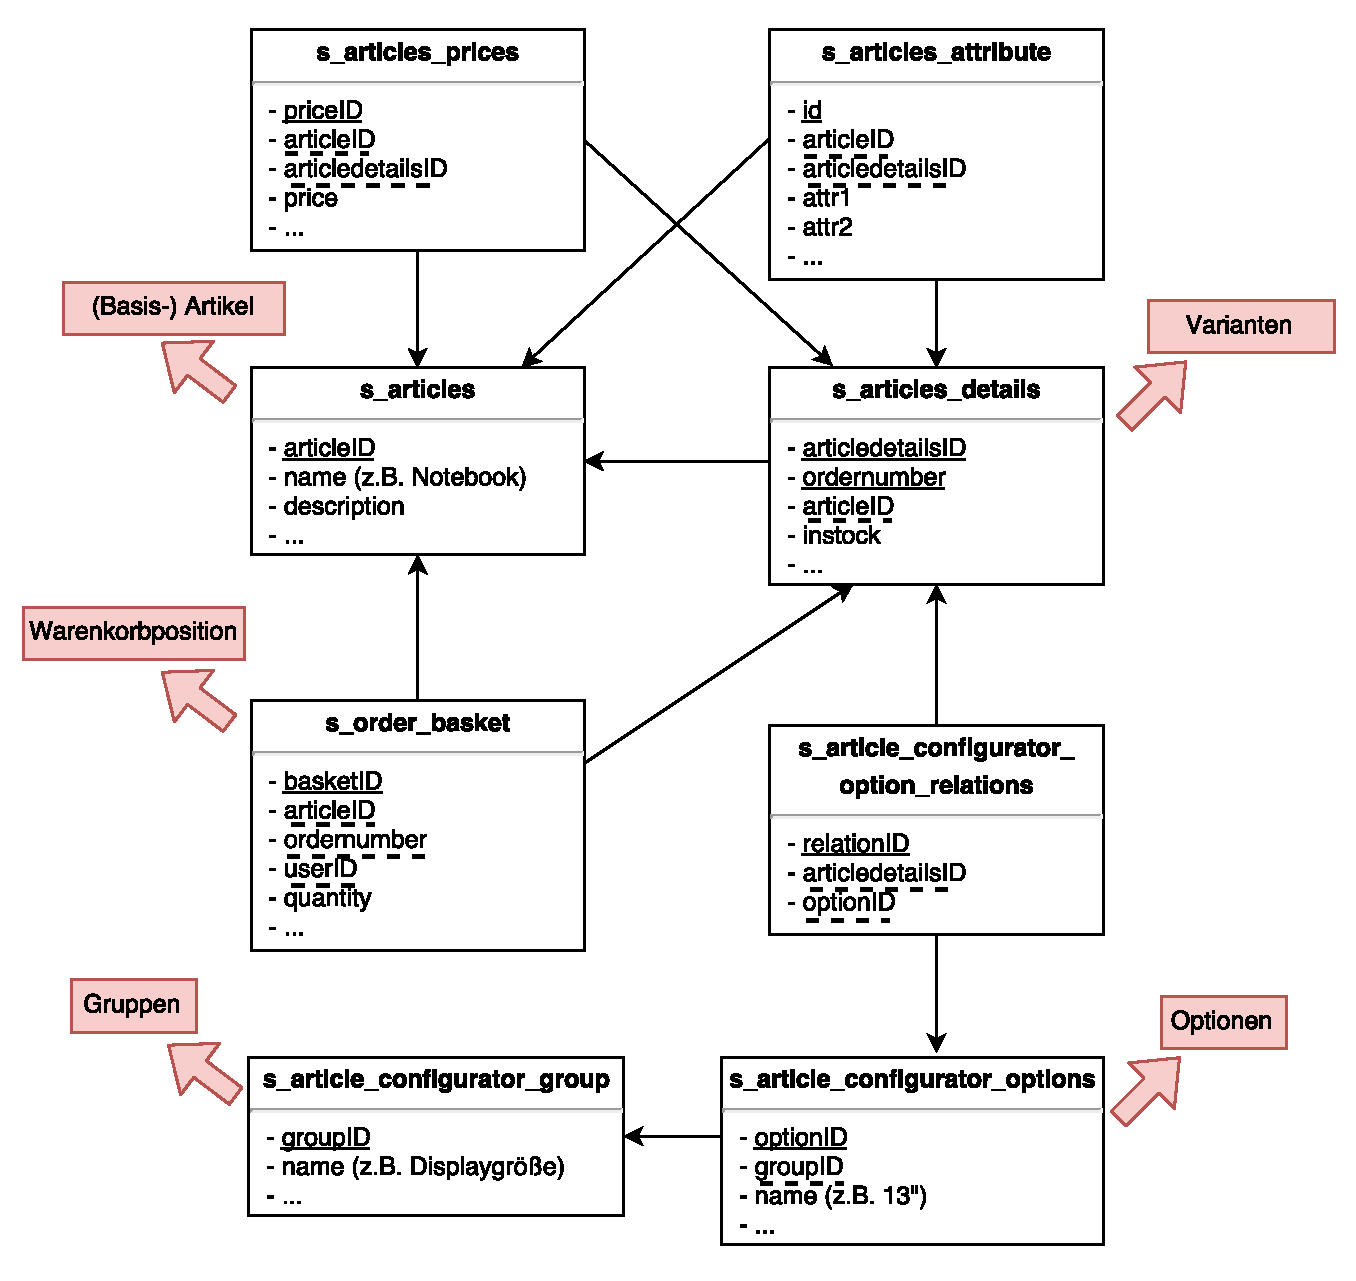
\includegraphics[width=0.7\linewidth]{Abbildungen/shopwareArtikelRelationenModell.pdf}
	\captionof{figure}[Ausschnitt des Relationenmodells von Shopware]{Ausschnitt des Relationenmodells von Shopware}
	\label{fig:shopwareArtikelRelationenModell}
\end{minipage}
\vspace{0.3em}

Abbildung \ref{fig:shopwareArtikelRelationenModell} zeigt einen Ausschnitt des Shopware-Datenbankschemas als Relationenmodell. Eine vollständige Übersicht ist \citet{shopwareDatabaseScheme} zu entnehmen. Auf der Abbildung sind die im Analysekapitel \ref{Shopsystem} verwendeten Begriffe rot zugeordnet. Dem Relationenmodell ist zu entnehmen, dass Artikel (\emph{s\_articles}) und deren Varianten (\emph{s\_articles\_details}) in unterschiedlichen Tabellen gespeichert werden. Artikel und Varianten stehen in einer 1-zu-n Beziehung. Dabei kennen Varianten ihren jeweiligen Basisartikel, aber nicht umgekehrt. Es ist anzumerken, dass auch zu einem nichtkonfigurierbaren Artikel zumindest eine Zeile in \emph{s\_articles\_details} angelegt wird\footnote{Solche Kardinalitäten können in einem Relationenmodell nicht ausgedrückt werden.}. Der Artikel steht dann mit einer Variante in einer 1-zu-1 Beziehung. Diese Variante ist damit automatisch immer die \emph{Basisvariante}\footnote{Der Begriff Basisvariante wurde in Kapitel \ref{shopwareEinkaufsvorgang} definiert}. Daraus lässt sich ableiten, dass in \emph{s\_articles} Informationen stehen, die für alle Varianten gelten (z.B. die allgemeine Produktbeschreibung \emph{description}) während \emph{s\_articles\_details} detailliertere Informationen enthält (z.B. der jeweilige Lagerbestand \emph{instock}). Es ist hervorzuheben, dass \emph{s\_articles\_details} zwei Primärschlüssel besitzt -- \emph{articledetailsID} und \emph{ordernumber}. Die \emph{articledetailsID} wird vom System vergeben, während die \emph{ordernumber} vom Administrator bestimmt werden kann. Somit ist die \emph{ordernumber} ein menschenlesbarer Identifikator, der vom Vertrieb dem Produktkatalog des Unternehmens zugeordnet werden kann.

Die Verbindung zwischen einer Variante und den Optionen (\emph{s\_article\_configurator\_options }), aus denen sie generiert wurde, wird über die Tabelle \emph{s\_article\_configurator\_option\_relations} hergestellt. Weder sind Optionen inhärenter Bestandteil einer Variante, noch besitzt \emph{s\_articles\_details} obligatorische Fremdschlüsselverweise auf \emph{s\_article\_configurator\_options}. Damit ist eine Variante nicht existentiell auf Optionen angewiesen. Daraus wird geschlussfolgert, dass während des Einkaufsprozesses Varianten dynamisch, d.h. bei Bedarf, generiert werden können.

Im Gegensatz dazu hat eine Warenkorbposition (\emph{s\_order\_basket}) einen obligatorischen Fremdschlüsselverweis auf eine Variante -- und ist damit von deren Existenz abhängig. Ein Warenkorbposition kann zeitlich nicht vor der zugehörigen Variante angelegt werden. Es wird geschlussfolgert, dass eine Variante noch nicht zum Beginn des Einkaufsvorgangs, aber spätestens beim Ablegen in den Warenkorb erstellt werden muss. Damit steht der zeitliche Spielraum für die dynamische Variantengenerierung fest.

\subsection{Einkaufsvorgang}
Abbildung \ref{fig:konzeptionEinkausvorgang1} stellt den neuen Einkaufsvorgang dar. Er entsteht aus dem Einkaufsvorgang in Abbildung \ref{fig:shopwareKonfigurationFlussdiagramm}, wenn folgende Sachverhalte berücksichtigt werden:
\begin{enumerate}
\item Es wird mit dem TCsite-Plugin kommuniziert (dargestellt als Wolken).
\item Varianten werden dynamisch angelegt.
\item Wird eine Warenkorbposition umkonfiguriert, entsteht keine neue Warenkorbposition. Stattdessen wird die entsprechende Warenkorbposition aktualisiert.
\end{enumerate}

\vspace{1em}
\begin{minipage}{\linewidth}
	\centering
	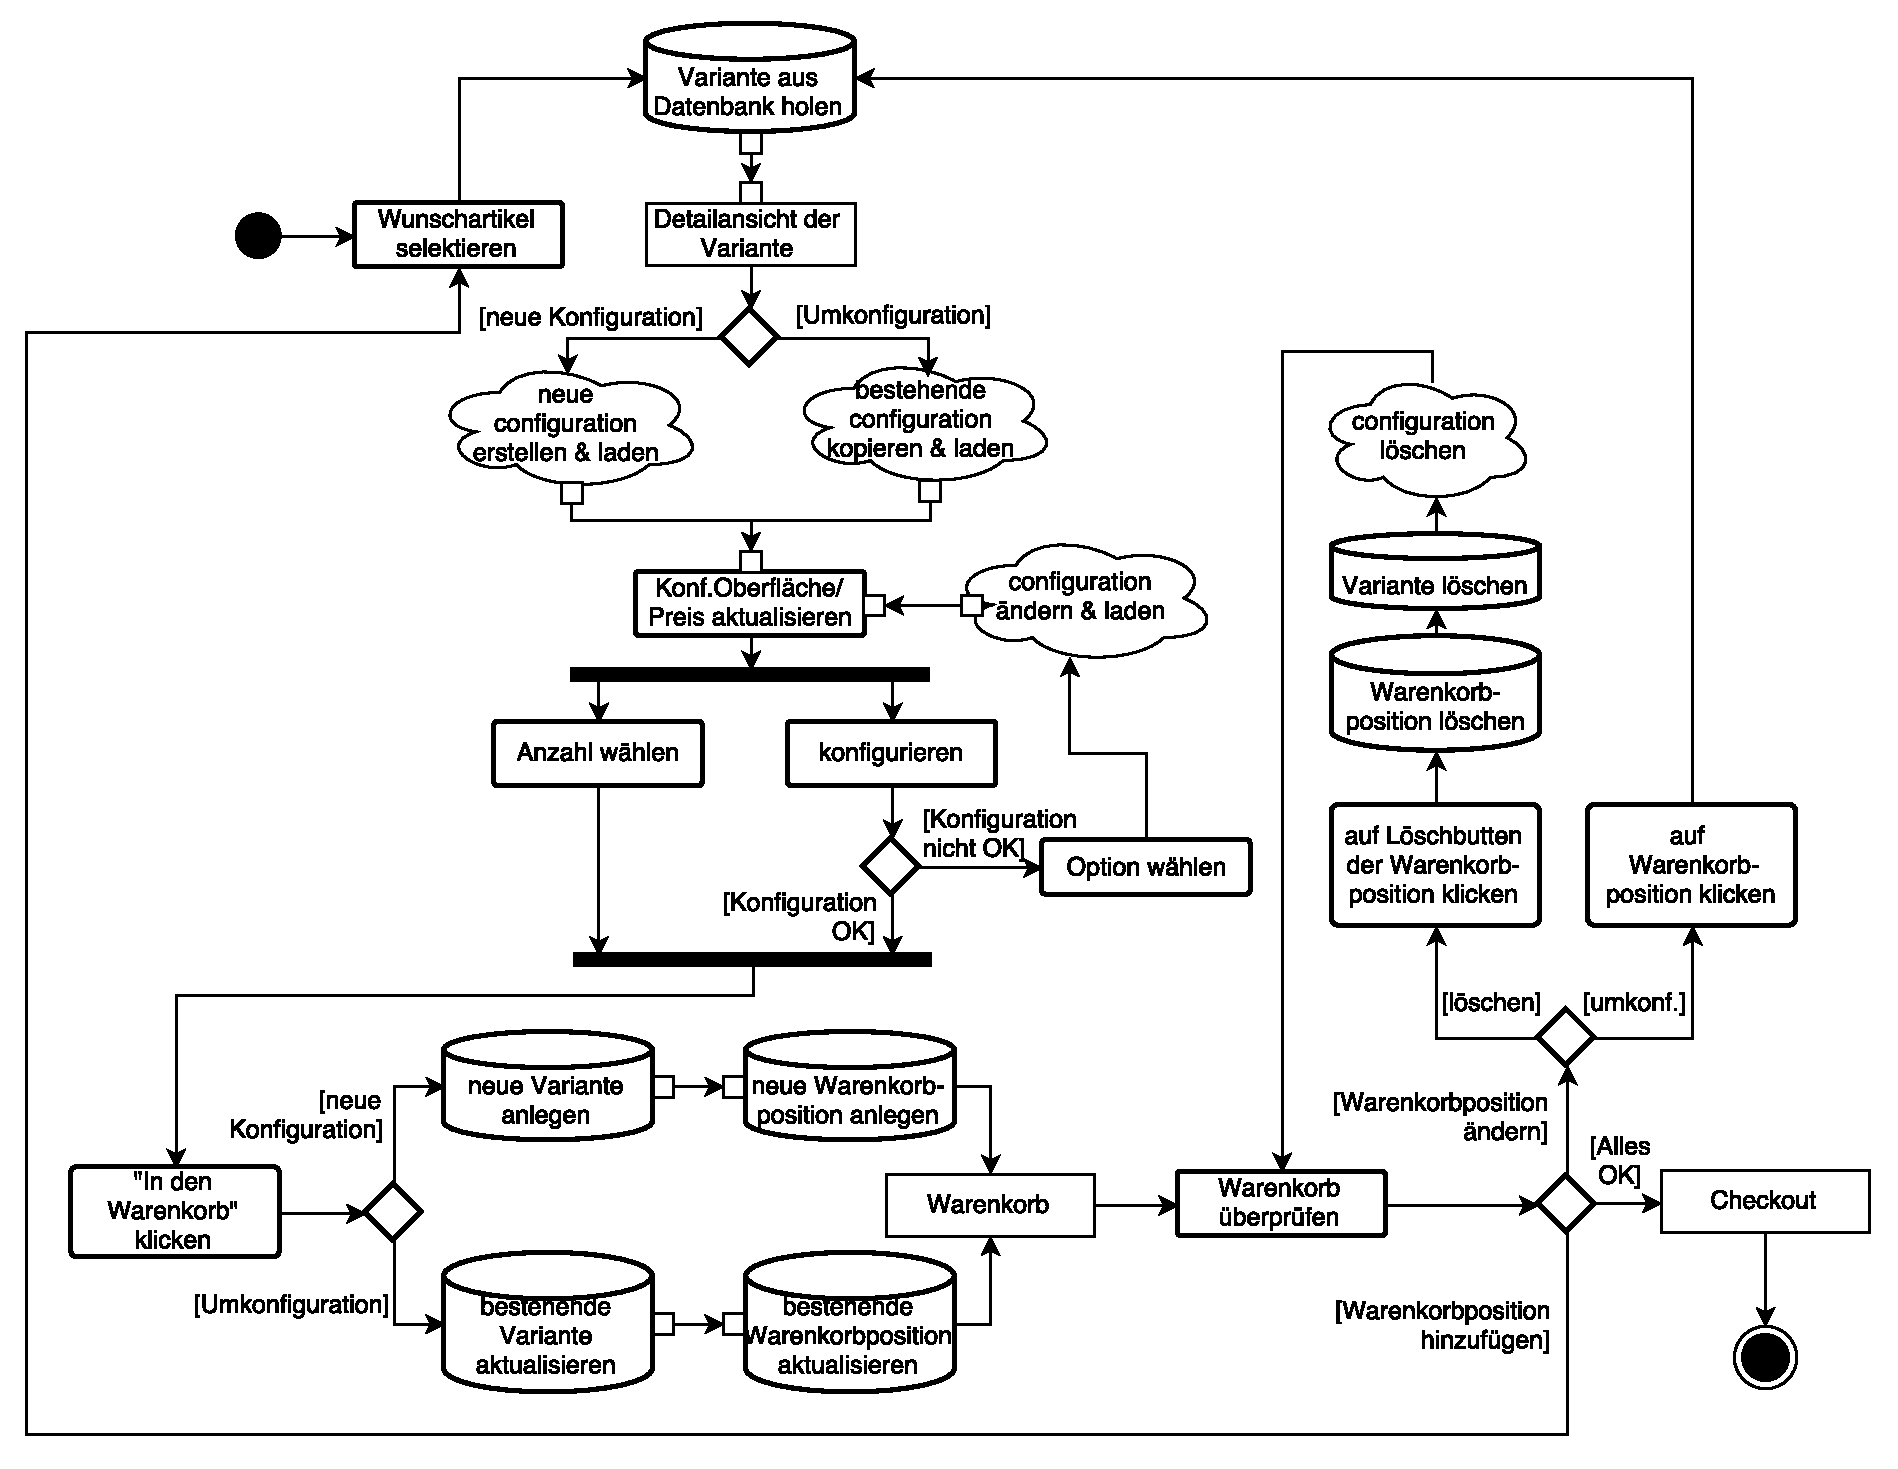
\includegraphics[width=1\linewidth]{Abbildungen/konzeptionEinkausvorgang1.pdf}
	\captionof{figure}[Aktivitätsdiagramm des Einkaufsvorgangs von Artikeln, die via Plugin konfiguriert werden]{Aktivitätsdiagramm des Einkaufsvorgangs von Artikeln, die via Plugin konfiguriert werden}
	\label{fig:konzeptionEinkausvorgang1}
\end{minipage}
\vspace{0.3em}

Das Aktivitätsdiagramm (Abbildung \ref{fig:konzeptionEinkausvorgang1}) bildet den \glqq roten Faden\grqq{} für die folgende Konzeption. Während der chronologischen Erläuterung des Einkaufsvorgangs werden die Daten und Prozesse erläutert, die vom Service bereit gestellt werden müssen. Gleichzeitig wird besprochen, welche Modifikationen der Shopware-Funktionalität vorgenommen werden müssen und welche der Erweiterungskonzepte aus Kapitel \ref{shopwareErweiterbarkeit} dafür jeweils in Frage kommen.

\subsubsection*{Artikellisting}
Der Einkaufsvorgang beginnt mit dem Auswählen des gewünschten Artikels. Das kann über verschiedene Wege passieren, zum Beispiel über das Artikellisting. Anhang \ref{app:shopwareArtikelListing} zeigt, dass dabei standardmäßig Preise angezeigt werden. Gemäß Anforderung SW.F16 dürfen konfigurierbare Artikel aber keinen Preis ausweisen.

Bereits zu diesem Zeitpunkt muss also vom System interpretierbar sein, welche Artikel via Plugin konfiguriert werden. Demzufolge muss bei den betreffenden Artikeln ein Hinweis über deren \glqq Konfigurierbarkeit\grqq{} hinterlegt werden. Das entspricht Anforderung SW.F17, gemäß derer im Backend die via Plugin konfigurierbaren Artikel markierbar sein müssen. Gleichzeitig fordert SW.F18 die Angabe, welchem TCsite-Produkt ein Shopware-Artikel entspricht. Im Folgenden wird diese Zuordnung als \emph{korrespondierendes TCsite-Produkt} bezeichnet. Es wird festgelegt: besitzt ein Artikel diese Zuordnung, ist es via Plugin konfigurierbar.

Zum Hinterlegen der Zuordnung wird eine Datenbank-Erweiterung genutzt. Konkret wird das in Kapitel \ref{shopwareErweiterbarkeit} angesprochene System der Attributtabellen verwendet. Plugins können Attributtabellen\footnote{Attributtabellen sind daran erkennbar, dass ihre Bezeichnung auf \emph{\_attributes} endet.} Spalten hinzufügen. Abbildung \ref{fig:shopwareArtikelRelationenModell} zeigt \emph{s\_articles\_attributes}, die Attributtabelle von Artikeln und ihren Varianten. Shopware legt zu jeder Zeile in \emph{s\_articles\_details} automatisch eine zugehörige Zeile in der Attributtabelle an. Es wird die Entwurfsentscheidung getroffen, der Tabelle die Spalte \emph{correspondingTcsiteProduct} hinzuzufügen.

Um diese Spalte im Backend befüllen zu können, wird ein entsprechendes Textfeld per \emph{Ext JS}-Erweiterung dem Artikelmenü (dargestellt in Anhang \ref{app:shopwareBackendArtikel}) hinzugefügt. In Kapitel \ref{shopwareErweiterbarkeit} wurde außerdem erwähnt, dass Smarty-Templates logische Einheiten via \emph{Blöcke} auszeichnen. Der Block namens \emph{frontend\_listing\_box\_article\_price\_default} beinhaltet den Preis eines Artikels im Artikellisting. Über eine Template-Erweiterung muss dieser Block ersetzt werden. Er soll künftig überprüfen, ob für den aktuell zu rendernden Artikel ein Eintrag in der Spalte \emph{correspondingTcsiteProduct} vorliegt und die Ausgabe entsprechend anpassen. Statt des Preises wird dann die Nachricht \glqq Preis entsprechend Konfiguration\grqq{} angezeigt. Somit werden die Anforderungen SW.F16, SW.F17 und SW.F18 erfüllt.

\subsubsection*{Detailseite}
Der Anwender befindet sich nun auf der Detailseite eines Artikels, der via Plugin konfigurierbar ist. Wie in Kapitel \ref{shopwareEinkaufsvorgang} besprochen, wird von Shopware die Basisvariante geladen und angezeigt. Der Artikel wurde im Backend nie als \emph{Varianten-Artikel} markiert. Darum wird nicht der Standard-Konfigurationsmechanismus von Shopware getriggert. Demzufolge wird auch kein Konfigurationsmenü wie in Anhang \ref{app:shopwareNotebookDetail} angezeigt. Aus Shopware-Sicht handelt es sich um einen normalen, nichtkonfigurierbaren Artikel.

Stattdessen startet nun der Konfigurationsprozess über das Shopware-Plugin. Dazu müssen Daten vom TCsite-Plugin geladen werden. Diese Daten werden im Rest der Konzeption unter dem Begriff \textbf{configuration} zusammengefasst. Aus Shopware-Sicht ist das ein \emph{Aggregat}\footnote{Das Aggregat als Ressourcentyp wurde in Kapitel \ref{Einschränkungen} vorgestellt}, welches alle Informationen zum Rendern der Konfigurationsoberfläche und zur Integration der entstehenden Variante in den Einkaufsvorgang enthält. Ob und wie dieses Aggregat als einzelne Ressourcen modelliert wird, ist der Verantwortungsbereich der späteren Webservice-Konzeption. Fest steht jetzt bereits, dass die \emph{configuration}-Ressource als JSON-Objekt repräsentiert wird. TCsite hat für Webcontroller eingebaute Komponenten zum serialisieren und deserialisieren von JSON-Objekten \citep{tactonTCsiteDevelopmentManual}.

\vspace{1em}
\begin{minipage}{\linewidth}
	\centering
	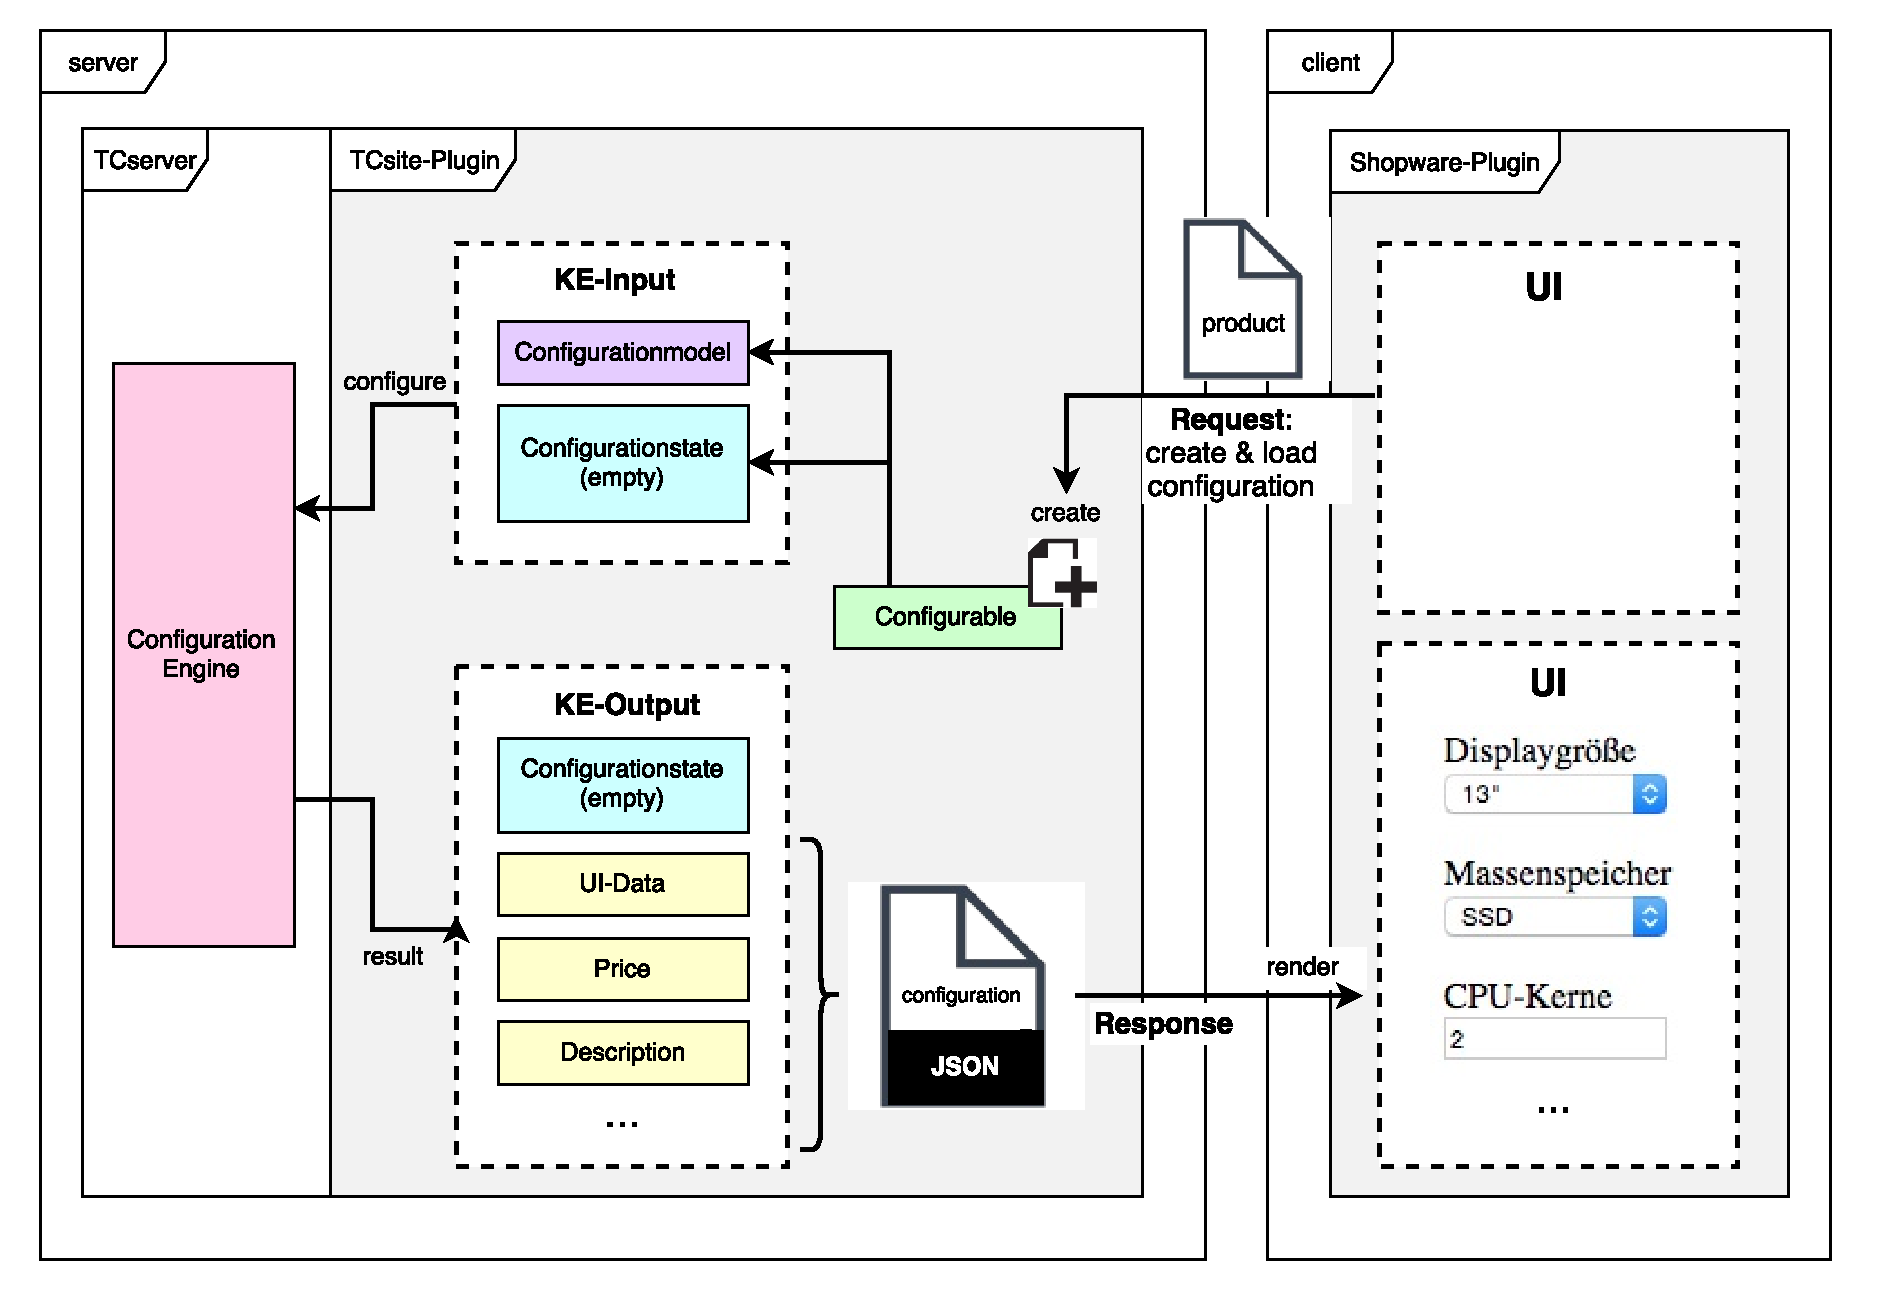
\includegraphics[width=1\linewidth]{Abbildungen/konzeptCreate.pdf}
	\captionof{figure}[Erstellen \& Laden einer neuen \emph{configuration}-Ressource]{Erstellen \& Laden einer neuen \emph{configuration}-Ressource}
	\label{fig:konzeptCreate}
\end{minipage}
\vspace{0.3em}

Abbildung \ref{fig:konzeptCreate} demonstriert den technischen Vorgang während der Aktivität \glqq neue \emph{configuration} erstellen \& laden\grqq{} (siehe Abbildung \ref{fig:konzeptionEinkausvorgang1}). Das Shopware-Plugin teilt dem TCsite-Plugin mit, für welches Produkt (z.B. Notebook) eine Konfiguration starten soll. Das TCsite-Plugin erstellt und speichert ein \emph{Configurable}-Objekt, welches in Verbindung mit dem entsprechenden Konfigurationsmodell und dem Konfigurationszustand steht. Der Konfigurationszustand ist leer, da zu diesem Zeitpunkt noch keine Optionen gewählt wurden. Es wird ein KE-Input definiert, der mit einem KE-Output beantwortet wird. Aus diesem werden die relevanten Informationen extrahiert, als JSON verpackt und dem Shopware-Plugin geschickt.

Der neuerstellten \emph{configuration} muss außerdem eine ID zugewiesen werden, die dem Shopware-Plugin in der Antwort mitgeteilt wird. Diese ID wird von nun an als \emph{configurationID} bezeichnet. Die Generierung und Semantik der ID wird während der Konzeption des TCsite-Plugins geklärt. Damit Shopwareseitig die ID für spätere Aufrufe gespeichert werden kann, muss die Datenbanktabelle \emph{s\_articles\_details} um die Spalte \emph{configurationID} ergänzt werden. Der Eintrag der ID folgt jedoch später.

Die Beschreibung des Aktivitätsdiagramms (Abbildung \ref{fig:konzeptionEinkausvorgang1}) wird fortgeführt\footnote{Die Erläuterung von \glqq bestehende \emph{configuration} kopieren \& laden\grqq{} erfolgt zu einem späteren Zeitpunkt.}. Es folgt das initiale Rendern der Konfigurationsoberfläche und die Aktualisierung der Preisanzeige mittels der Daten aus der \emph{configuration}, welche in der HTTP-Antwort übertragen wurden. Hierfür werden Template-Erweiterungen genutzt. Der Smarty-Block \emph{frontend\_detail\_index\_detail} zeichnet den Bereich der Detailseite aus, welcher das Artikelbild enthält (siehe Anhang \ref{app:shopwareNotebookDetail}). Unterhalb wird die Konfigurationsoberfläche angehangen. Außerdem wird die Preisanzeige aktualisiert. Für diese Vorgänge wird DOM-Manipulation und clientseitige Logik benötigt. Das bedeutet, es müssen Javascript-Dateien eingebunden werden. Hierfür steht der Smarty-Block \emph{frontend\_index\_header\_javascript} zur Verfügung.

Die Analyse des Konfigurationsprozesses in TCsite (Kapitel \ref{TCsiteKonfigurationsprozess}) hat ergeben, dass dieser in drei Phasen abläuft. Dabei wurde beschrieben, dass erst in der letzten Phase der Preis aus dem KE-Output extrahiert wird. Oben wurde jedoch dargestellt, dass Preisinformationen bereits beim initialen Aufbau der Konfigurationsoberfläche benötigt werden. Demzufolge läuft der Konfigurationsprozess im Integrationsszenario nicht phasenbasiert ab, sondern wird nach jedem Aufruf der Konfigurationsengine als potentiell abgeschlossen betrachtet.

\subsubsection*{Konfigurationsprozess}
Es folgt der Konfigurationsprozess. Entsprechend Anforderung SW.F02 interagiert der Anwender nun mit der Konfigurationsoberfläche. Das bedeutet er wählt Optionen, tätigt Eingaben, wechselt Steps etc. Abbildung \ref{fig:konzeptChange} stellt die Kommunikation zwischen dem Shopware-Plugin und dem TCsite-Plugin nach jeder Nutzerinteraktion dar.

\vspace{1em}
\begin{minipage}{\linewidth}
	\centering
	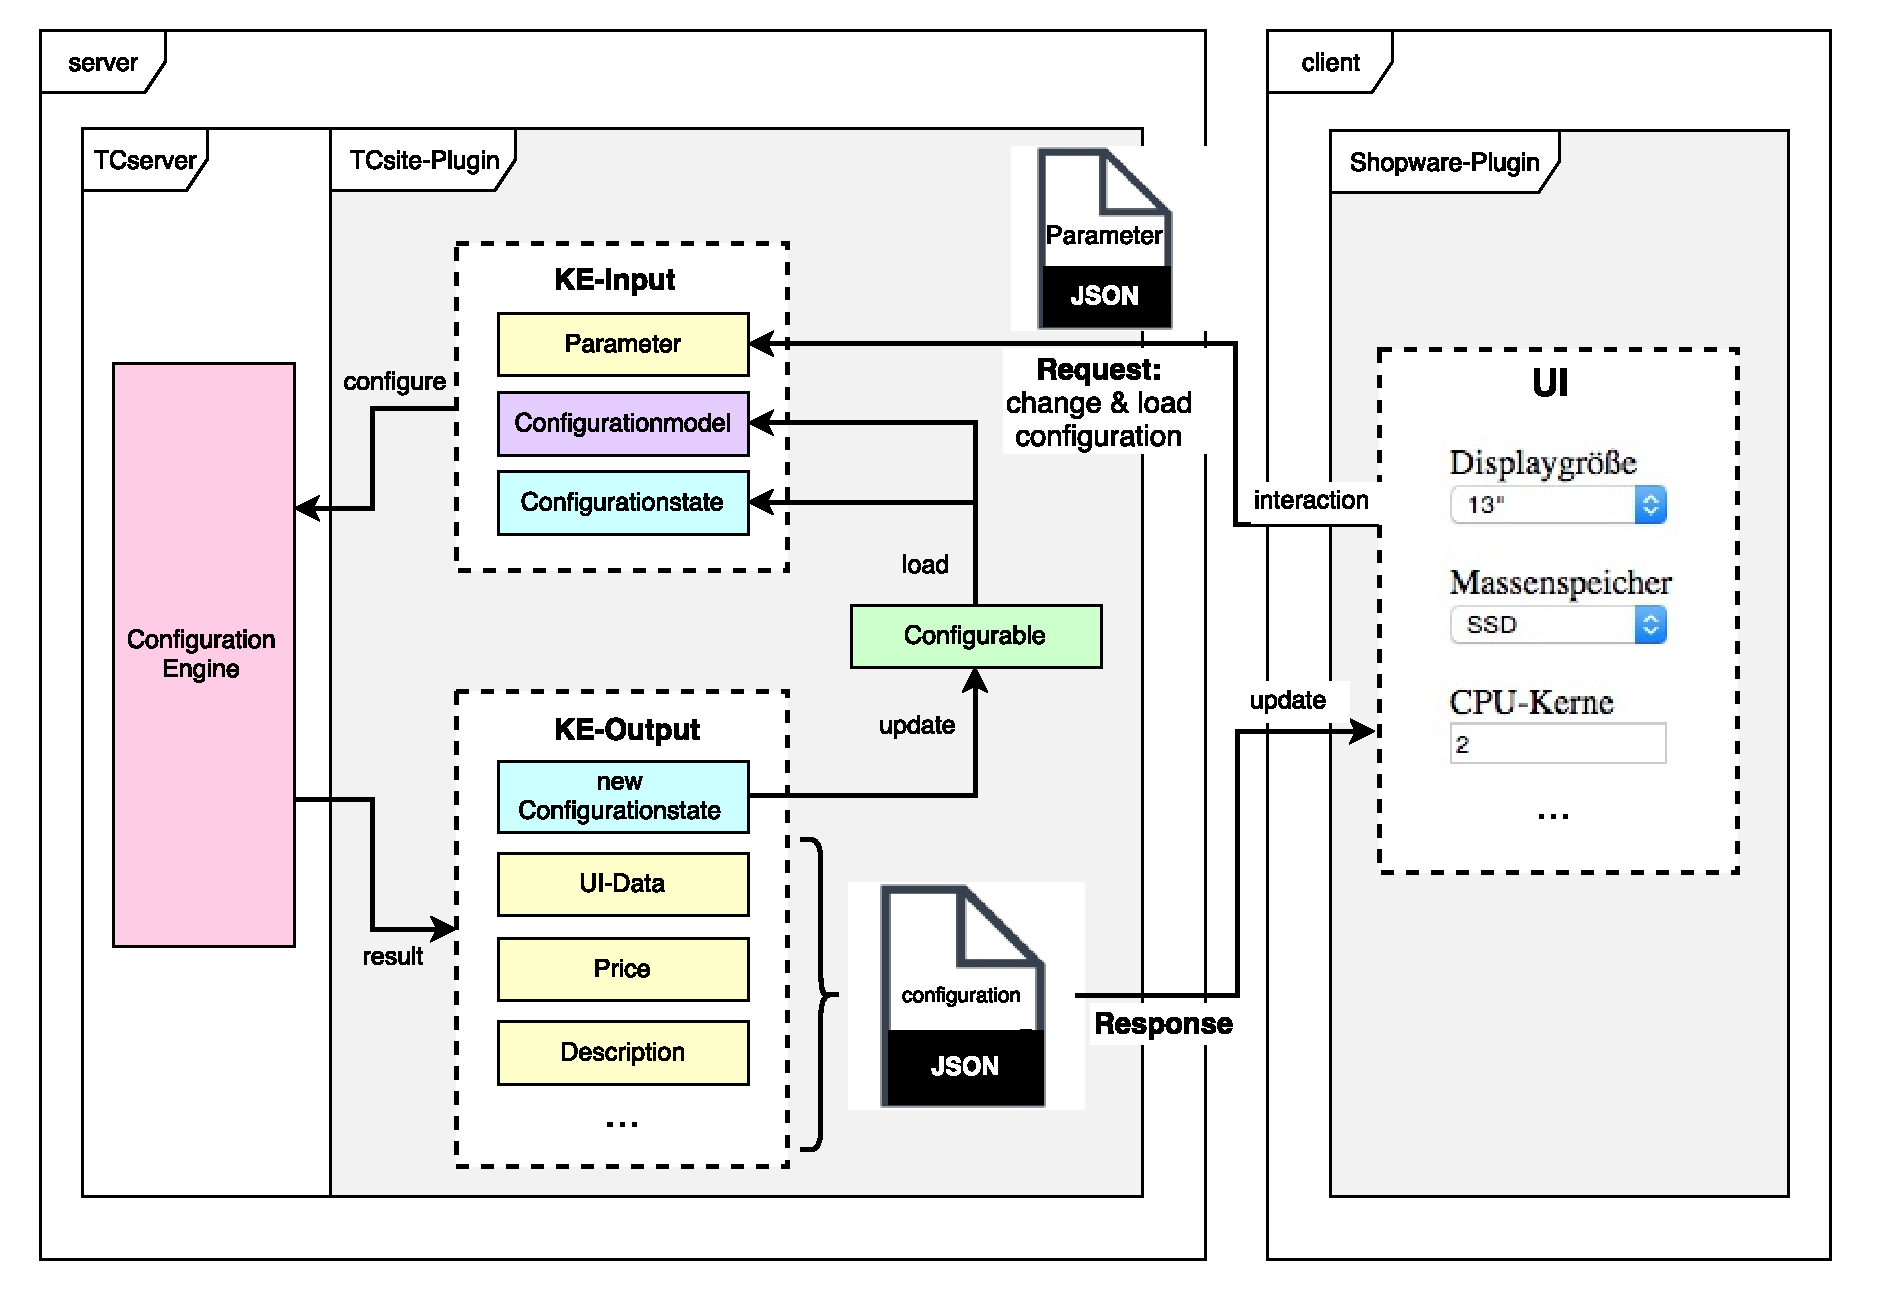
\includegraphics[width=0.9\linewidth]{Abbildungen/konzeptChange.pdf}
	\captionof{figure}[Ändern \& Laden der \emph{configuration}-Ressource]{Ändern \& Laden der \emph{configuration}-Ressource}
	\label{fig:konzeptChange}
\end{minipage}
\vspace{0.3em}

In Folge einer Nutzerinteraktion übermittelt das Shopware-Plugin den Eingabeparameter an das TCsite-Plugin. Außerdem muss die \emph{configurationID} übertragen werden, welche das Shopware-Plugin beim initialen Anfordern der \emph{configuration} erhalten hat. So kann das TCsite-Plugin zuordnen, auf welches \emph{Configurable} sich der Eingabeparameter bezieht und einen KE-Input definieren. Der KE-Output enthält den neuen Konfigurationszustand. Das \emph{Configurable} wird entsprechend aktualisiert und gespeichert. Aus den übrigen relevanten Daten generiert das TCsite-Plugin die \emph{configuration}-Ressource und verschickt diese in der HTTP-Antwort. Das Shopware-Plugin nimmt die \emph{configuration} entgegen und aktualisiert die Konfigurationsoberfläche und Preisanzeige.

Jede Interaktion des Anwenders mit der Oberfläche löst den eben beschriebenen Prozess aus. Dieser Kreislauf wiederholt sich solange, bis der Anwender im letzten Step angekommen und mit allen Optionen zufrieden ist. Gemäß Anforderung SW.F06 wird der \glqq In den Warenkorb\grqq{}-Button erst jetzt aktiviert, wodurch der Konfigurationsprozess abgeschlossen werden kann.

Insgesamt werden so die Anforderungen SW.F01\footnote{Die Bereitstellung einer Konfigurationsoberfläche.} und SW.F04\footnote{Die Anzeige des aktuellen Preises.} erfüllt. SW.0F2 fordert außerdem, dass der Konfigurationsprozess äquivalent zu TCsite verläuft. Die genaue Nachempfindung der Abläufe ist ein Implementierungsdetail, welches in Kapitel \ref{Umsetzung} angerissen wird.

\subsubsection*{Dynamische Variantengenerierung}
Der Klick auf den \glqq In den Warenkorb\grqq{}-Button führt bei einer neuen Konfiguration zum Anlegen einer Warenkorbposition (entspricht Anforderung SW.F05)\footnote{Die Unterscheidung dieses Falles von einer Umkonfiguration wird später erläutert.}. Standardmäßig wird durch den Button die \emph{ajaxAddArticleCart}-Action des Checkout-Controllers ausgelöst\footnote{Die Controller-Terminologie wurde in Kapitel \ref{shopwareArchitektur} vorgestellt}. In der Action wird erst die Warenkorbposition angelegt und dann der Warenkorb angezeigt. In der Vorbetrachtung dieses Entwurfskapitels wurde festgestellt, dass bei der Erstellung einer Warenkorbposition die zugehörige Variante bereits existieren muss. Der Konfigurationsprozess fand aber statt, während auf der Detailseite noch die Basisvariante geladen war. Die aus dem Konfigurationsprozess resultierende Variante muss also erst noch generiert werden. Die Analyse der Shopware-Erweiterbarkeit in Kapitel \ref{shopwareErweiterbarkeit} hat ergeben, dass Controller-Actions überschreibbar sind. \emph{ajaxAddArticleCart} wird also durch eine vom Shopware-Plugin bereitgestellte Funktion ersetzt, um die dynamische Variantengenerierung zu hinzuzufügen.

Abbildung \ref{fig:dynamischeVariantengenerierung} visualisiert die Vorgänge in der \emph{ajaxAddArticleCart} des Plugins. Zunächst wird eine neue Variante angelegt, die sich auf den gleichen Artikel wie die Basisvariante bezieht. Das bedeutet, es wird eine neue Zeile in der Tabelle \emph{s\_articles\_details} mit einem Fremdschlüsselverweis auf \emph{s\_articles} erzeugt (siehe Abbildung \ref{fig:shopwareArtikelRelationenModell}). Die \emph{ordernumber} (d.h. der menschenlesbare Primärschlüssel) wird dabei automatisch generiert. Außerdem wird die entsprechende \emph{configurationID} in der Tabelle \emph{s\_articles\_details} hinterlegt. So ist die Variante mit der \emph{configuration}-Ressource verknüpft, die während des Konfigurationsprozesses verwendet wurde. Der Preis wird in der Tabelle \emph{s\_articles\_details} angelegt und der Variante zugeordnet.

\vspace{1em}
\begin{minipage}{\linewidth}
	\centering
	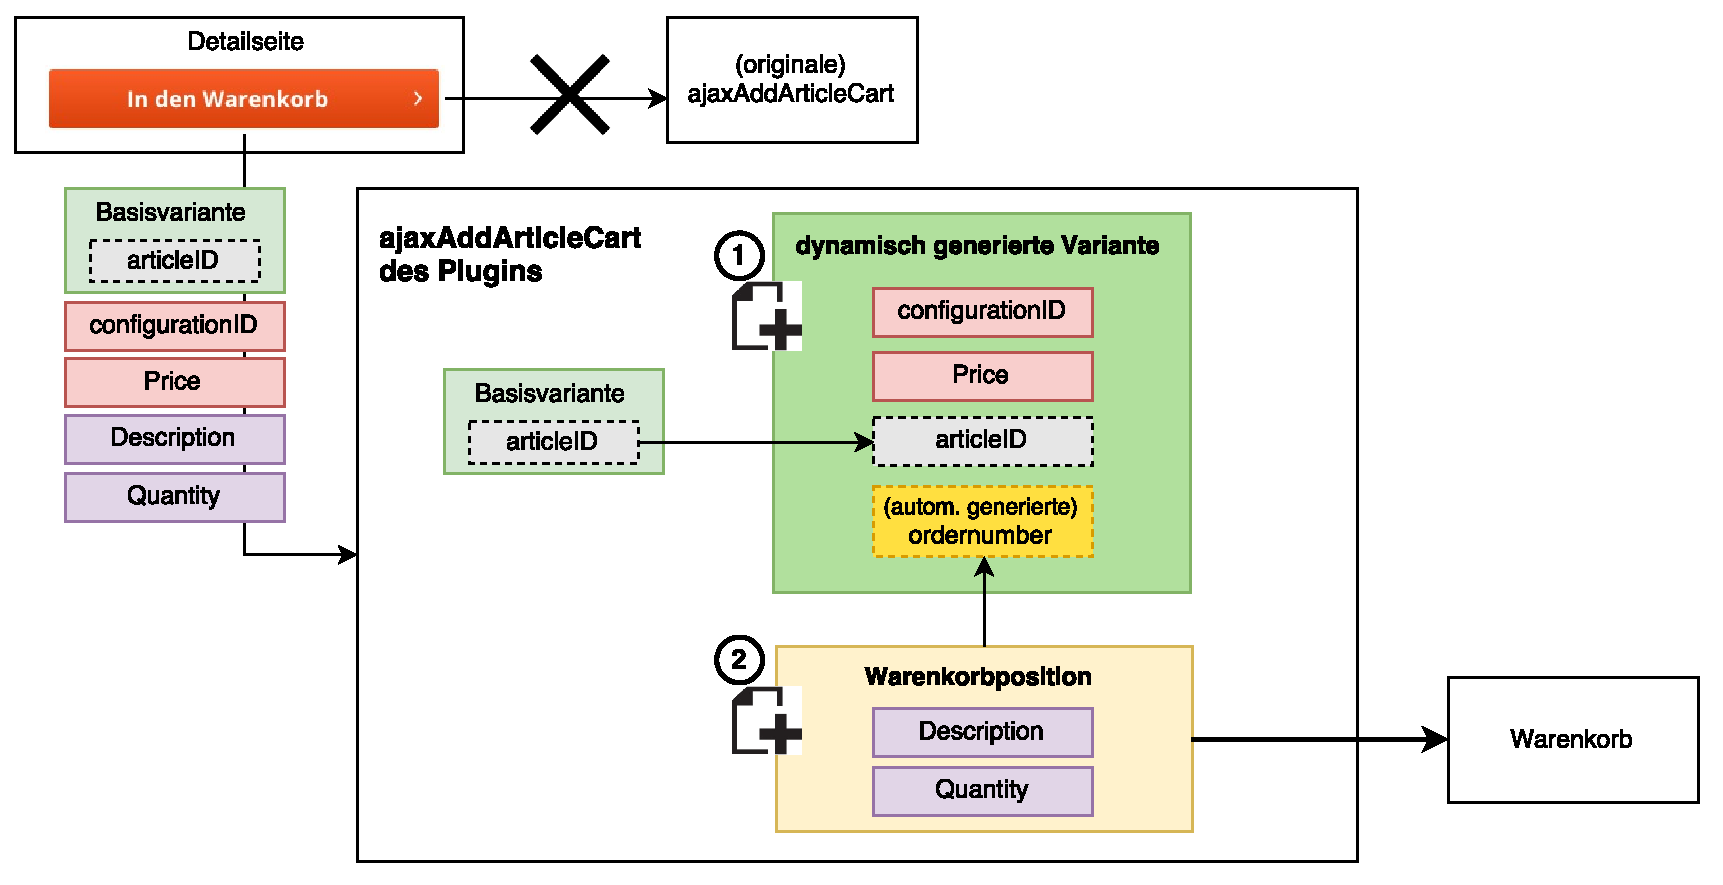
\includegraphics[width=1\linewidth]{Abbildungen/dynamischeVariantengenerierung.pdf}
	\captionof{figure}[Dynamische Variantengenerierung]{Dynamische Variantengenerierung}
	\label{fig:dynamischeVariantengenerierung}
\end{minipage}
\vspace{0.3em}

Jetzt wird die Warenkorbposition in der entsprechenden Anzahl eingetragen. Dementsprechend wird eine neue Zeile in der Tabelle \emph{s\_articles\_basket} erzeugt. Zum Erfüllen der Anforderung SW.F07 wird der Name der Warenkorbposition (Spalte \emph{articlename}) zu einer Kurzbeschreibung\footnote{Die Kurzbeschreibung stammt ebenfalls aus der \emph{configuration}-Ressource.} der Variante geändert (z.B. \glqq Notebook OSX Yosemite 4GB RAM\grqq{}).

Zusammengefasst muss die überschriebene \emph{ajaxAddArticleCart}-Action im Gegensatz zur Standardmethode drei zusätzliche Informationen verarbeiten -- die \emph{configurationID}, den Preis und die Kurzbeschreibung.

\subsubsection*{Warenkorb}
Die aktuelle Station des Einkaufsvorgangs ist der Warenkorb (siehe Abbildung \ref{fig:konzeptionEinkausvorgang1}). Möchte der Anwender weitere Artikel konfigurieren, schließt er den Warenkorb und beginnt den Einkaufsvorgang von vorne. Damit wiederholt sich der bisher beschriebene Prozess. Ist der Anwender mit einer Warenkorbposition unzufrieden, kann er diese löschen (SW.F13) oder umkonfigurieren (SW.F08).

Im Gegensatz zum ursprünglichen Einkaufsvorgang (siehe Abbildung \ref{fig:shopwareKonfigurationFlussdiagramm}) hat das Löschen einer Warenkorbposition weitere Löschvorgänge zur Folge. Eine Variante wurde nur erstellt, um als Bezugspunkt einer Warenkorbposition zu dienen. Das Löschen einer Position macht auch die zugehörige Variante obsolet. Dementsprechend wird diese aus der Datenbank entfernt. Durch die in Abbildung dargestellten \ref{fig:shopwareArtikelRelationenModell} Fremdschlüsselverweise werden auch die entsprechenden Zeilen aus \emph{s\_articles\_prices} und \emph{s\_articles\_details}  gelöscht. Gleichzeitig wird die zugehörige \emph{configuration} funktionslos. Dementsprechend muss ein Löschbefehl an das TCsite-Plugin abgesetzt werden.

Der Löschvorgang einer Warenkorbposition wird in Shopware von der Methode \emph{sDeleteArticle} des Moduls \emph{sBasket} realisiert (siehe Abbildung \ref{fig:tcsiteLowLevel}). Weder handelt es sich um eine Controller-Action, noch enthält die Funktion Notify-Events. Entsprechend der Erläuterung der logischen Erweiterungen in Kapitel \ref{shopwareErweiterbarkeit} muss also auf das Hooksystem zurückgegriffen werden. \emph{sDeleteArticle} wird eine Funktion nachgeschaltet, worin das Löschen der entsprechenden Variante und \emph{configuration} nachgeholt wird. SW.F13 wird so erfüllt.

\subsubsection*{Umkonfiguration}
Durch einen Klick auf eine Warenkorbposition gelangt der Anwender zur Detailansicht der Variante. Dies entspricht soweit dem Shopware-Standard und erfordert keine zusätzliche Logik. Somit wird Anforderung SW.F09 erfüllt. Zusätzlich muss die Konfigurationsoberfläche wieder aufgebaut und der Preis abgeholt werden, um SW.F10 zu erfüllen. Beim Anlegen der Variante wurde die zugehörige \emph{configurationID} gespeichert. Somit kann die entsprechende \emph{configuration} geladen werden. Dies entspricht der Aktivität \glqq bestehende \emph{configuration} kopieren und laden\grqq{} aus Abbildung \ref{fig:konzeptionEinkausvorgang1}.

\vspace{1em}
\begin{minipage}{\linewidth}
	\centering
	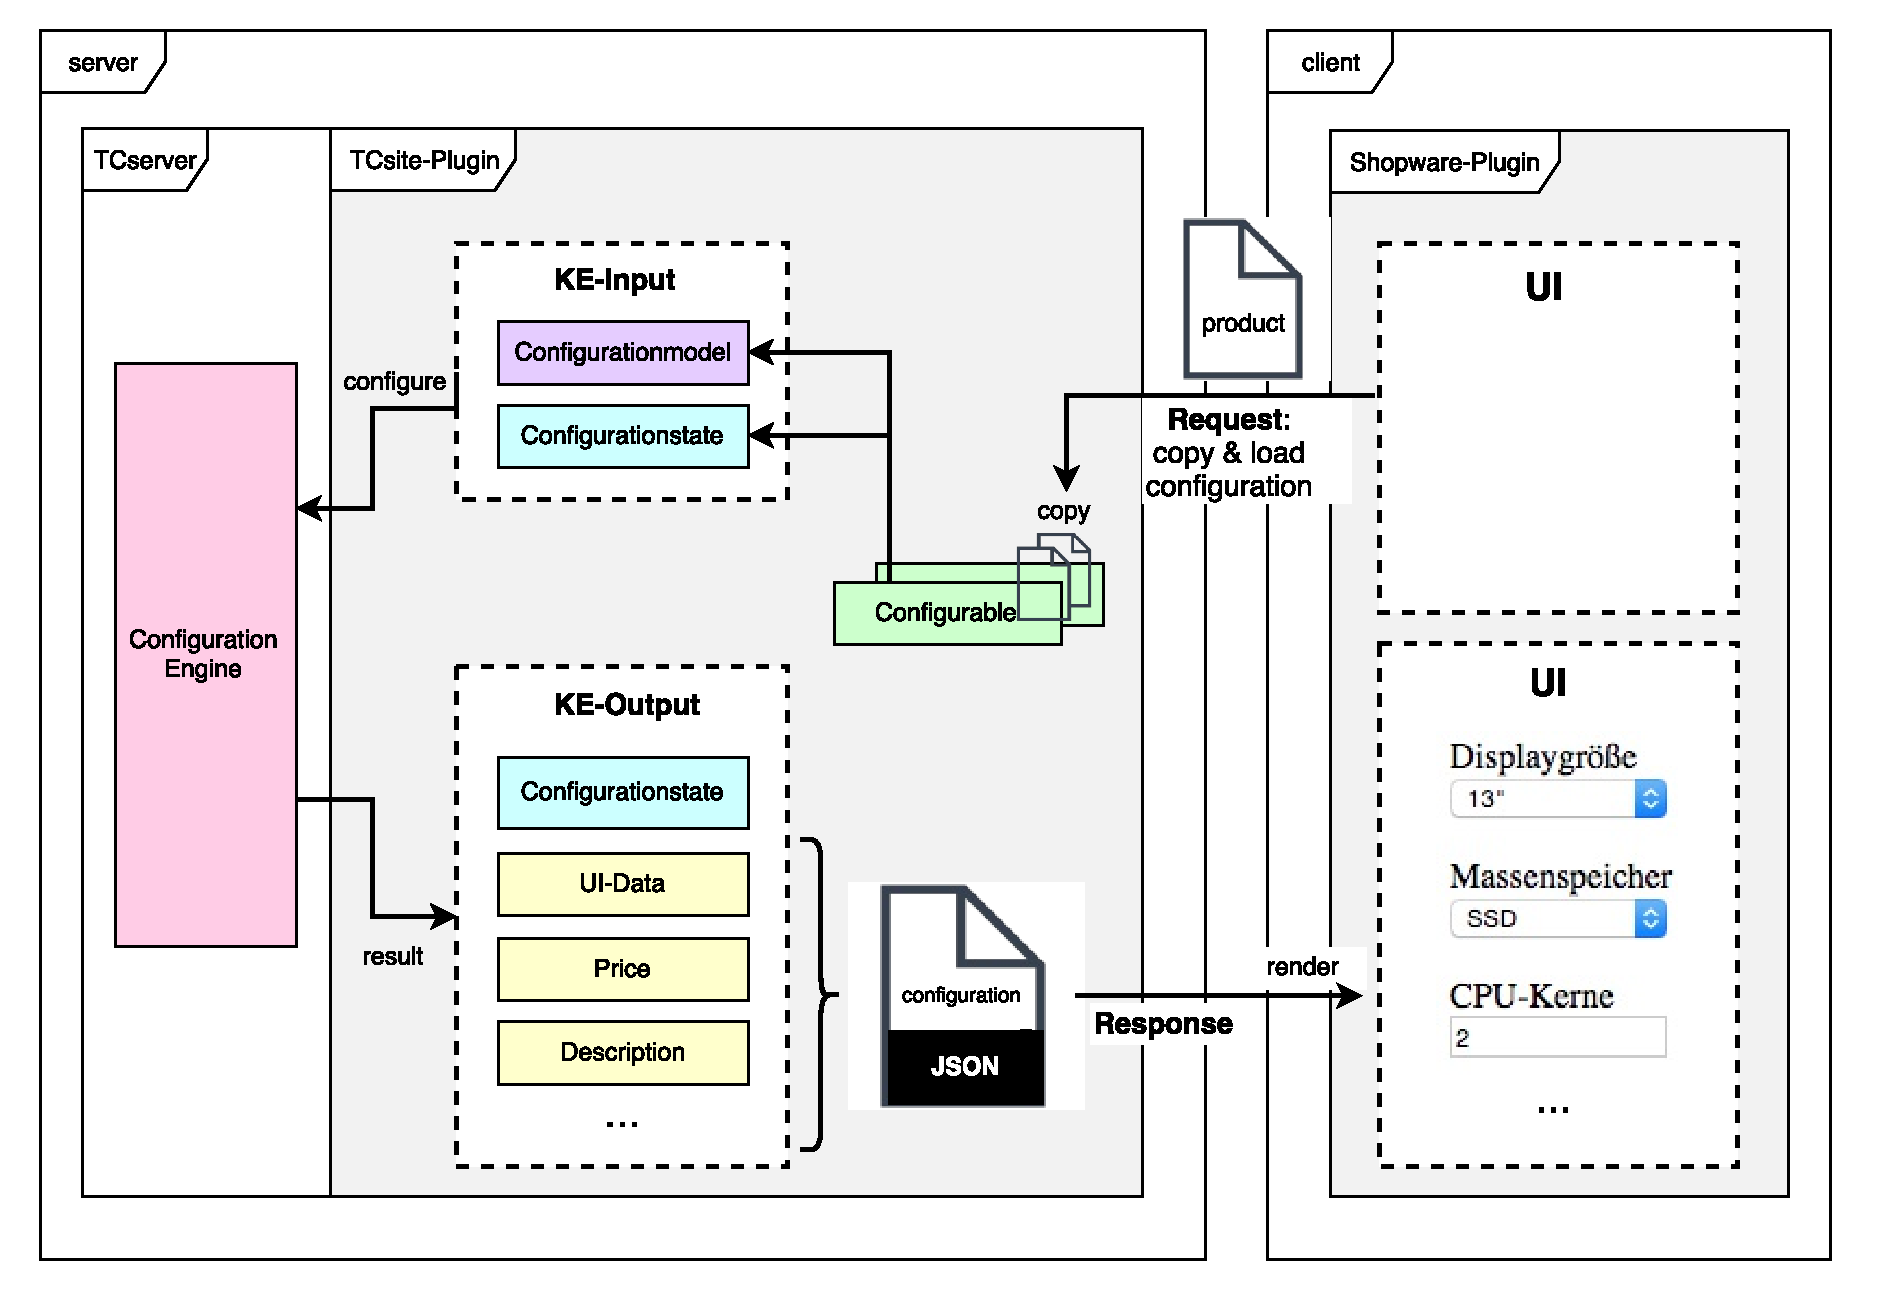
\includegraphics[width=1\linewidth]{Abbildungen/konzeptCopy.pdf}
	\captionof{figure}[Kopieren \& Laden einer bestehenden \emph{configuration}]{Kopieren \& Laden einer bestehenden \emph{configuration}}
	\label{fig:konzeptCopy}
\end{minipage}
\vspace{0.3em}

Abbildung \ref{fig:konzeptCopy} stellt den dabei ablaufenden Prozess dar. Er entspricht insofern der Aktivität \glqq neue \emph{configuration} erstellen \& laden\grqq{} (siehe Abbildung \ref{fig:konzeptCreate}), als dass der KE-Input ohne Eingabeparameter verarbeitet wird. Dementsprechend ist der Konfigurationszustand vor und nach dem Aufruf der Konfigurationsengine gleich. Jedoch geschieht der Umkonfigurationsprozess auf einer Arbeitskopie, wobei der Konfigurationszustand der ursprünglichen \emph{configuration} übernommen wird. Grund dafür ist Anforderung SW.F11, gemäß derer die Umkonfiguration erst abschließend vom Anwender bestätigt werden muss. Es ist also möglich, dass der Anwender zunächst andere Optionen wählt, die Änderungen aber verwerfen möchte (z.B. indem er die Detailseite ohne Bestätigung der Umkonfiguration verlässt). Ohne das Anfertigen einer Arbeitskopie würde im Falle des Verwerfens eine Diskrepanz zwischen einer Variante und der zugeordneten \emph{configuration} entstehen.

Die Beschriftung des \glqq In den Warenkorb\grqq{}-Buttons wird auf \glqq Neue Konfiguration speichern\grqq{} geändert. So wird darauf hingewiesen, dass der Button ein geändertes Verhalten aufweist. Die entsprechende Warenkorbposition wird nicht inkrementiert, sondern aktualisiert. Die Aktualisierung betrifft den Preis (Spalte: \emph{price}; Tabelle: \emph{s\_articles\_prices}), die Beschreibung (Spalte: \emph{articlename}; Tabelle: \emph{s\_order\_basket}) und die Anzahl (Spalte: \emph{quantity}; Tabelle: \emph{s\_order\_basket}). Außerdem muss die \emph{configurationID} auf die der Arbeitskopie aktualisiert werden, da diese nun den aktuellen Konfigurationszustand enthält.

Zwar wurde die Beschriftung des \glqq In den Warenkorb\grqq{}-Buttons geändert, er triggert aber immer noch die gleiche Controller-Action. Darum kann zur Implementierung des neuen Verhalten die bereits überschriebene \emph{ajaxAddArticleCart}-Funktion genutzt werden. In dieser muss unterschieden werden, ob es sich um eine neue Konfiguration oder eine Umkonfiguration handelt. Letzteres ist dann der Fall, wenn für die Variante bereits eine \emph{configurationID} hinterlegt ist.

Der vorangegangen Erläuterung ist zu entnehmen, dass zwei Varianten nie auf inhaltliche Gleichheit überprüft werden. Auch wenn der Anwender zweimal hintereinander genau die gleiche Konfiguration vornimmt, werden separate Warenkorbpositionen angelegt, da jede im Zusammenhang mit einer eigenen \emph{configuration} steht. Somit wird Anforderung SW.F12\footnote{Jede Variante muss im Warenkorb eine eigene Position darstellen.} erfüllt.

\textbf{Bestellung}\\
Die erstellten Varianten gehen als normale Artikel in den Bestellprozess ein (SW.F14). Durch die Entscheidung, die Kurzbeschreibung einer Variante zum Namen der Warenkorbposition zu machen, erscheint diese auch in der Bestellbestätigung (SW.F15).

Im Eingang dieses Kapitels wurde erwähnt, dass über die \emph{ordernumber} einer Variante (Tabelle: \emph{s\_articles\_details}) die bestellte Warenkorbposition vom Vertrieb dem Produktkatalog zugeordnet werden kann. Die \emph{ordernumber} wurde im eben dargestellten Ablauf jedoch automatisiert generiert. Allein durch die Bestellbestätigung ist also noch nicht klar, welche Varianten hier eigentlich beauftragt wurden. Zur Lösung des Problems gibt es zwei Ansätze:
\begin{enumerate}
\item Die Kurzbeschreibung der Variante ist aussagekräftig genug. Das ist allerdings nur bei Varianten mit wenig Optionen realistisch.
\item Die \emph{configurationID} ermöglicht die Auswertung der Daten, die bei TCsite mit der jeweiligen Variante im Zusammenhang stehen. Genaueres zur dieser Vorgehensweise wird in der Konzeption des TCsite-Plugins besprochen.
\end{enumerate}

\subsection{Zusammenfassung}
Vorausgehend wurden die notwendigen Erweiterungen entlang des Einkaufsvorgangs aus Abbildung \ref{fig:konzeptionEinkausvorgang1} beschrieben und begründet. Implizit wird so Anforderung SW.F03\footnote{Die Integration der Varianten in Einkaufsvorgang.} erfüllt. Im Folgenden werden noch einmal alle Erweiterungen nach Typ sortiert und zusammengefasst:
 
\begin{enumerate}
\item \textbf{Daten-Erweiterungen:}
\begin{enumerate}[(a)]
\item Hinzufügen von Variantenattributen\\
Tabelle: \emph{s\_articles\_details}, Spalten: \emph{correspondingTcsiteProduct}/\emph{configurationID}
\end{enumerate}
\item \textbf{Template-Erweiterungen:}
\begin{enumerate}[(a)]
\item Ersetzen des Preises im Artikellisting\\Smarty-Block: \emph{frontend\_listing\_box\_article\_price\_default}
\item Einfügen der Konfigurationsoberfläche in die Detailseite\\Smarty-Block: \emph{frontend\_detail\_index\_detail}
\item Einfügen von clientseitiger Logik mittels Einbindung von Javascript-Dateien in der Detailseite\\Smarty-Block: \emph{frontend\_index\_header\_javascript}
\item Einfügen eines Textfeldes im Artikelmenü des Backends zur Eingabe des korrespondierenden TCsite-Produkts\\Block: \emph{frontend\_index\_header\_javascript}
\end{enumerate}
\item \textbf{logische Erweiterungen:}
\begin{enumerate}[(a)]
\item Überschreiben der Controller-Action zum Hinzufügen von Warenkorbpositionen\\
Controller: \emph{Checkout}, Action: \emph{ajaxAddArticleCart}
\item \glqq Hooken\grqq{} der Methode zum Löschen von Warenkorbartikeln\\
Modul: \emph{sBasket}, Methode: \emph{sDeleteArticle}
\end{enumerate}
\end{enumerate}

Anforderung SW.F19\footnote{Die Einstellung im Backend, unter welcher URI das TCsite-Plugin erreichbar ist.} schlägt die Brücke zur folgenden Konzeption des TCsite-Plugins. Dieses ist ein Webservice und hat dementsprechend eine Adresse im Web. Die Adresse muss dem Shopware-Plugin noch bekannt gegeben werden. Shopware erlaubt dem Administrator im Backend neben der Aktivierung und Deaktivierung von Plugins auch dessen \glqq Konfiguration\grqq{}\footnote{Konfiguration bedeutet in diesem Kontext, dass Einstellungen an Plugins vorgenommen werden können.} über Formularfelder \citep{shopwarePluginKonfiguration}. Durch die Einrichtung des Textfeldes \glqq Webadresse des TCsite-Plugins\grqq{} wird SW.F19 erfüllt. Alle funktionalen Anforderungen des Shopware-Plugins wurden somit entworfen.

\section{TCsite-Plugin}
\label{TCsite-Plugin}
Äquivalent zur Konzeption des Shopware-Plugins findet zunächst eine technische Vorbetrachtung statt. Der vorausgehende Entwurf hat gezeigt, dass jeder Prozess im TCsite-Plugin mit der Verarbeitung eines \emph{Configurable}-Objekts verbunden ist. Im Folgenden wird untersucht, wie der Zugriff auf das Objekt realisiert wird. Daraus resultieren Erkenntnisse, die entscheidend für die Konzeption der Serviceendpunkte sind.

\subsection{Vorbetrachtung}
\label{TCsite-PluginVorbetrachtung}
Abbildung \ref{fig:konzeptConfigurableUML} visualisiert die Beziehungen zwischen \emph{Quotations}, \emph{QuotationItems} und \emph{Configurables}. Eine \emph{Quotation} besitzt eine beliebige Anzahl \emph{QuotationItems}. Jedes \emph{QuotationItem} steht in einer 1-zu-1 Beziehung mit einem \emph{Configurable}. \citet{tactonTCsiteDevelopmentManual} rät davon ab, ein \emph{Configurable} direkt per Konstruktor zu erstellen. Zur vollen Einsatzbereitschaft des Objekts seien weitere initialisierende Schritte notwendig. Welche, verrät die Dokumentation nicht. Stattdessen wird auf die Methode \emph{createAndAddQuoteItem} der Serviceklasse \emph{QuotationService} verwiesen. Diese erstellt zu einer gegebenen \emph{Quotation} ein \emph{QuotationItem} mit dem entsprechenden \emph{Configurable}. Dabei werden alle initialisierenden Schritte übernommen. Die Implementierung von TCsite zwingt so zur zusätzlichen Verwaltung von \emph{Quotations} und \emph{QuotationItems}, auch wenn nur das \emph{Configurable} für den Konfigurationsprozess unmittelbar relevant ist.

\vspace{1em}
\begin{minipage}{\linewidth}
	\centering
	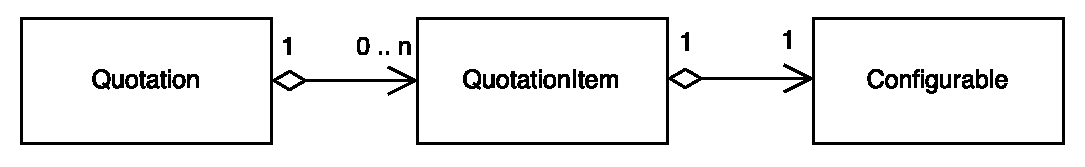
\includegraphics[width=1\linewidth]{Abbildungen/konzeptConfigurableUML.pdf}
	\captionof{figure}[Beziehungen zwischen \emph{Quotations}, \emph{QuotationItems} und \emph{Configurables}]{Beziehungen zwischen \emph{Quotations}, \emph{QuotationItems} und \emph{Configurables}}
	\label{fig:konzeptConfigurableUML}
\end{minipage}
\vspace{1em}

\emph{Quotations} und \emph{QuotationItems} sind nicht nur Mittel zum Zweck der Erstellung eines \emph{Configurables}. Das Auswerten von Preisinformationen und die Zusammenstellung der Kurzbeschreibung wird ebenfalls durch API-Methoden des \emph{QuotationService} realisiert. Die hierfür zuständigen Methoden benötigen neben dem KE-Output und dem \emph{Configurable} auch die zugehörige \emph{Quotation} und das \emph{QuotationItem}. Zusammenfassend wird festgestellt, dass jede Verarbeitung eines \emph{Configurable} nur im Kontext einer \emph{Quotation} möglich ist.

Es wird die Entwurfsentscheidung getroffen, zu jedem \emph{Configurable} genau eine \emph{Quotation} anzulegen und zu persistieren (entspricht Anforderung TC.F02). Diese Entscheidung hat zwei Vorteile:
\begin{enumerate}
\item Da jede \emph{Quotation} nur ein \emph{Configurable} enthält, identifiziert die ID der \emph{Quotation} gleichzeitig das \emph{Configurable}. Damit ist nun klar, was die \emph{configurationID} im Entwurf des Shopware-Plugins ist -- die ID einer \emph{Quotation}.
\item In der Quotation-View von TCsite (Abbildung \ref{fig:tcsiteQuotationNumbered}) existiert ein Index, der alle \emph{Quotations} auflistet. Wird eine Variante in Shopware bestellt, kann so über die hinterlegte \emph{configurationID} die zugehörige \emph{Quotation} in TCsite geöffnet werden. In der \emph{Quotation} befindet sich nur ein \emph{QuotationItem} -- und zwar die Variante, die der Shopwarekunde bestellt hat. So wird das Problem gelöst, welches im Abschnitt \glqq Bestellung\grqq{} der Konzeption des Shopware-Plugins angesprochen wurde -- der Vertrieb kann interpretieren, welche Varianten in Shopware eigentlich bestellt wurden.
\end{enumerate}

Durch Anforderung TC.NF03 steht bereits fest, dass das TCsite-Plugin einen Webservice implementiert, der den Einschränkungen des REST-Architekturstils gerecht werden soll. Entsprechend der vorgestellten Theorie in Kapitel \ref{REST} müssen die Ressourcen mit deren Repräsentationen und Verknüpfungen (Hypermedia) entworfen werden. Weitergehend wird entschieden, unter welcher URI und mit welchen Methoden die Interaktion mit den Ressourcen stattfindet.

\subsection{Ressourcen}
Im Entwurf des Shopware-Plugins wurde bereits die Ressource \emph{configuration} modelliert. Entsprechend der Ressourcentypisierung, die in Kapitel \ref{Einschränkungen} vorgestellt wurde, handelt es sich um ein \emph{Aggregat}. Es enthält unterschiedliche Daten -- Preisinformationen (Anforderung TC.F05), eine Kurzbeschreibung für die Warenkorbposition (Anforderung TC.F06) und die Datengrundlage zum Rendern der Konfigurationsoberfläche (Anforderung TC.F01). Diese Informationen könnten auch auf mehrere Ressourcen aufgeteilt werden. Da das vorliegende Konzept des Shopware-Plugins aber alle Daten zum gleichen Zeitpunkt benötigt, würde eine feingranularere Ressourcenmodellierung nur zu mehr Serveraufrufen führen.

Außerdem wurde festgestellt, dass eine \emph{configuration} die eigene ID enthalten muss (entspricht Anforderung TC.F03). Das spielt bei den Aktivitäten \glqq neue \emph{configuration} erstellen \& laden\grqq{} sowie \glqq bestehende \emph{configuration} kopieren \& laden\grqq{} eine Rolle (siehe Abbildung \ref{fig:konzeptionEinkausvorgang1}). Hier erfährt das Shopware-Plugin erst in der Serverantwort die \emph{configurationID} für die weitere Kommunkation. In diesem Grenzfall verweist eine Ressource auf sich selbst, was dennoch eine Orientierungshilfe für den Clienten darstellt. Somit wird die REST-Einschränkung \emph{Hypermedia} erfüllt.

In der Konzeption des Shopware-Plugins wurde festgelegt, dass die Ressourcen in Form von JSON repräsentiert werden. Listing \ref{lst:configuration} skizziert die Form der \emph{configuration} am Notebook-Beispiel mit exemplarischen Werten. Die Daten für die Konfigurationsoberfläche (\emph{ui-data}) sind ein komplexes Konstrukt. TCsite stellt Methoden bereit, die den KE-Output auslesen und die \emph{ui-data} durch die Ineinanderschachtelung von JSON-Objekten als serialisierten Baum darstellen. Die dabei stattfindenden Prozesse sind für den Plugin-Entwickler nicht einsehbar und werden in der Arbeit nicht weiter ausgeführt. Letztendlich muss das Shopware-Plugin diesen Baum traversieren und so die Konfigurationsoberfläche aufbauen.

\vspace{1em}
\begin{lstlisting}[caption=Beispiel einer \emph{configuration}, label=lst:configuration]
{
	"price": 420,
	"summary": "hallo"
	"ui-data": {
			steps: [...],
			groups: [...],
			...
	 },
	"configurationID": "1024"
}
\end{lstlisting}

\subsection{Serviceendpunkte}
Im nächsten Schritt werden die URIs der Ressourcen entworfen und festgelegt, welche Methoden diese jeweils unterstützen.

Zunächst einmal hat das Plugin einen Basispfad im Web, der Teil jeder Ressourcen-URI ist. Wie dieser aussieht, hängt von der Adresse der TCsite-Installation ab. Im Folgenden wird mit der exemplarischen URI \glqq http://tcsite-uri.de/path-to-the-plugin/\grqq{} gearbeitet. Als Adresse für die \emph{configuration} wird entschieden, den Namen der Ressource als Pfadende zu verwenden (z.B. \glqq http://tcsite-uri.de/path-to-the-plugin/configuration\grqq{}).

Der Identifikator einer Ressource ist ein Parameter, der Teil der URI ist. Laut \citet{tilkov11} ist es Geschmackssache, ob er als Pfad-Parameter (z.B. \glqq http://tcsite-uri.de/path-to-the-plugin/configuration/1024\grqq{}) oder Query-Parameter (z.B. \glqq http://tcsite-uri.de/path-to-the-plugin/configuration?id=1024\grqq{}) entworfen wird. Da im Laufe der folgenden Erläuterung noch weitere Query-Parameter eingeführt werden, wird aus Konsistenzgründen letztere Variante gewählt.

Als nächstes müssen die HTTP-Methoden definiert werden, welche die Ressource unterstützt. Die Wolken in Abbildung \ref{fig:konzeptionEinkausvorgang1} zeigen alle Operationen, die vom Service implementiert werden müssen. Im Folgenden wird unter Berücksichtigung der HTTP-Spezifikation (siehe Tabelle \ref{tab:restMethoden}) besprochen, auf welche HTTP-Methode jede der Operation abgebildet werden darf. Außerdem werden bei Bedarf zusätzliche Query-Paramter definiert.

\begin{enumerate}
\item[\textbf{\emph{configuration} löschen:}] Entspricht semantisch der HTTP-Methode DELETE.
\begin{addmargin}[25pt]{0pt} 
Beispiel: Ein DELETE-Request an\\
\glqq http://tcsite-uri.de/path-to-the-plugin/configuration?id=1024\grqq{}
\\löscht die \emph{Quotation} mit der ID 1024 und alle assoziierten Objekte (\emph{Configurable} etc.).
\end{addmargin}
\item[\textbf{neue \emph{configuration} erstellen \& laden:}] Das Anlegen einer Ressource entspricht semantisch der HTTP-Methode PUT. Allerdings fordert die Spezifikation, dass die Ressource künftig unter der gleichen Adresse erreichbar ist, unter der sie via PUT angelegt wurde. Zum Erstellungszeitpunkt kennt der Client die URI der entstehenden \emph{configuration} aber noch nicht. Diese wird ihm erst in der Antwort mittels der \emph{configurationID} mitgeteilt. Die Operation entspricht also eher der Methode POST im engeren Sinne, d.h. das Anlegen einer Ressource unter einer vom Service bestimmten URI.\\Da im Folgenden noch weitere Operationen POST verwenden, wird der Query-Parameter \emph{operation} eingeführt. Durch diesen wird dem Webservice mitgeteilt, welche Operation im Falle eines POST erwünscht ist. Das Erstellen einer \emph{configuration} bekommt das Schlüsselwort \emph{create} zugeordnet. Weiterhin muss kommuniziert werden, für welches TCsite-Produkt eine \emph{configuration} erstellt werden soll. Hierfür wird der Query-Parameter \emph{product} eingeführt.
\begin{addmargin}[25pt]{0pt} 
Beispiel:
\\Ein POST-Request an \glqq http://tcsite-uri.de/path-to-the-plugin/
\\configuration?operation=create\&product=notebook\grqq{}\\
erstellt eine neue Notebook-Konfiguration.
\end{addmargin}
\item[\textbf{bestehende \emph{configuration} kopieren \& laden:}] Es existiert keine HTTP-Methode, die semantisch dem Kopieren entspricht. Die Operation muss also auf POST abgebildet werden, da sie die einzige Methode ohne sichtbare Semantik ist. Für den \emph{operation}-Parameter wird das Schlüsselwort \emph{copy} gewählt.
\begin{addmargin}[25pt]{0pt} 
Beispiel:\\
Ein POST-Request an \glqq http://tcsite-uri.de/path-to-the-plugin/
\\configuration?id=1024\&operation=copy\grqq{}
\\kopiert die \emph{Quotation} mit der ID 1024.
\end{addmargin}
\item[\textbf{bestehende \emph{configuration} ändern \& laden:}] Bedeutet die Verarbeitung eines Eingabeparameters, während der Anwender in Shopware konfiguriert (entspricht Anforderung TC.F04). Semantisch wird dadurch ein Prozess ausgedrückt. Prozesse werden der Methode POST (im weiteren Sinne) zugeordnet. Für den \emph{operation}-Parameter wird das Schlüsselwort \emph{change} gewählt, da sich der Konfigurationszustand innerhalb des zugehörigen \emph{Configurables} ändert. Weiterhin muss der Methode der Eingabeparameter mitgeteilt werden. Die Codierung dieser Information ist ein Implementierungsdetail und wird in der Arbeit nicht weiter besprochen\footnote{Genaueren Aufschluss gibt \citet{tactonTCsiteDevelopmentManual} im Abschnitt \glqq ConfigurationActionBean\grqq{}.}. Um nicht zu viele Query-Parameter zu erzeugen, wird der Eingabeparameter als JSON codiert und im Entity-Body des HTTP-Requests mitgeschickt.
\begin{addmargin}[25pt]{0pt} 
Beispiel:\\
Ein POST-Request an \glqq http://tcsite-uri.de/path-to-the-plugin/
\\configuration?id=1024\&operation=change\grqq{}
\\mit einer JSON-Payload, in welcher die Wahl des Betriebssystems 'OSX Yosemite' codiert wird, setzt diese Option unverhandelbar im Konfigurationszustand (falls sie nicht im Konflikt mit einer anderen Option steht).
\end{addmargin}
\end{enumerate}

\subsection{Zusammenfassung}
Tabelle \ref{tab:konzeptRestZusammenfassung} fasst die Spezifikation des  \emph{configuration}-Ressourcenendpunkts tabellarisch zusammen.

\vspace{1em}
\begin{minipage}{\linewidth}
	\centering
	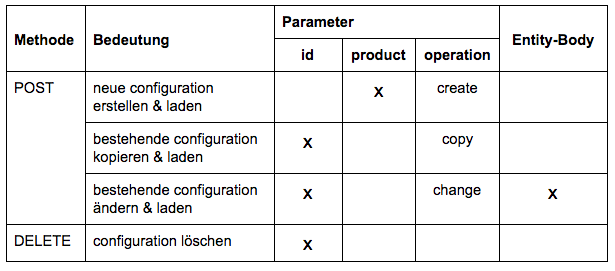
\includegraphics[width=1\linewidth]{Abbildungen/konzeptRestZusammenfassung.png}
	\captionof{table}[Zusammenfassung der REST-Schnittstelle]{Zusammenfassung der REST-Schnittstelle}
	\label{tab:konzeptRestZusammenfassung}
\end{minipage}
\vspace{1em}

\chapter{Umsetzung}
\label{Umsetzung}
Im Folgenden findet ein Überblick über die Herangehensweise an die Umsetzung statt. Der Ablauf der Implementierung wird episodisch besprochen. Währenddessen werden ausgewählte Umsetzungsdetails vorgestellt. Jeder Abschnitt schließt mit einer Zusammenfassung des jeweiligen Ergebnisses ab. Voraussetzung zum Verständnis dieses Kapitels sind Kenntnisse über die Grundlagen der Webprogrammierung.

Im Gegensatz zur Konzeptionsreihenfolge wurde die Entwicklung mit dem TCsite-Plugin begonnen. Zunächst wurde eine Webcontroller-Erweiterung zum Testen der Verbindung geschrieben. Um den Zugriff auf TCsite-Funktionalitäten zu ermöglichen, musste der in Kapitel \ref{TCsiteArchitektur} erwähnte Integrationsuser angelegt und dem Plugin zugewiesen werden. Als Testclient diente eine einfache HTML-Seite, die XMLHttpRequests (d.h. die HTTP-Kommunikation mit Javascript) via \ac{AJAX} an den Webcontroller absetzt. Hierbei hat sich herausgestellt, dass \ac{CORS} beachtet werden muss. Im Folgenden wird die Problematik näher erläutert.

Browser implementieren ein Sicherheitskonzept namens \ac{SOP}. Dieses verhindert XMLHttpRequests an eine andere Domain als diejenige, von welcher der Request stammt. Beispielsweise würde eine Anfrage von der Domain \glqq http://shopware-test.de\grqq{} an \glqq http://tcsite-test.de\grqq{} blockiert werden. Die Serverantwort käme zwar an, jedoch wird vom Browser vor dessen Auswertung der HTTP-Header ‘Access-Control-Allow-Origin‘ kontrolliert. Durch diesen wird signalisiert, welche Domains mit der angeforderten Ressource interagieren dürfen. Ist die Domain des Clienten nicht eingetragen, wirft der Browser einen Fehler \citep{mozillaCORS}. Eine genauere Darstellung des Sachverhalts ist Anhang \ref{app:mozillaCORS} zu entnehmen. Sicherheitsaspekte wurden bei den nichtfunktionalen Anforderungen der Anforderungsanalyse (siehe Kapitel \ref{nichtfunktionaleAnforderungen}
) noch nicht berücksichtigt. Darum wurde der Tomcat von TCsite so eingestellt, dass er Requests von allen Domains akzeptiert. Das Ergebnis dieses Abschnitts ist die Herstellung einer Client-Server Kommunikation zwischen unterschiedlichen Domains.

Nachdem die Kommunikation zwischen dem Testclienten und dem TCsite-Plugin erfolgreich funktioniert hat, wurde das Erstellen einer \emph{Quotation} samt \emph{QuotationItem} und \emph{Configurable} umgesetzt. Als Testprodukt diente dabei eine Umsetzung der exemplarischen Notebook-Konfiguration. Im nächsten Schritt wurde die Generierung und Verarbeitung eines KE-Inputs erprobt. Der KE-Input wird in TCsite durch die Klasse \emph{ConfigurationActionBean} implementiert. Aus dem KE-Output wurden die Daten für den initialen Aufbau der Konfigurationsoberfläche mittels Standardmethoden von TCsite zusammengestellt. Diese wurden als JSON-Payload an den Testclienten in der HTTP-Antwort zurückgeschickt. Während der Konzeption des TCsite-Plugins wurde erwähnt, dass die Daten für die Konfigurationsoberfläche als serialisierter Baum übertragen werden. Der Baum wird von TCsite als \emph{grouptree} bezeichnet. Die erste Version der \emph{configuration}-Ressource enthält also nur UI-Daten. Das Ergebnis dieses Abschnitts ist ein erster Austausch von Ressourcen.

Danach wurde das Wählen von Optionen innerhalb des TCsite-Plugins simuliert. Dabei wurde mit verschiedenen Werten für die Attribute der \emph{ConfigurationActionBean} experimentiert. Im Testclienten war anhand der Serverantwort beobachtbar, ob der KE-Input erfolgreich von der Konfigurationsengine verarbeitet werden konnte, welche Optionen gesetzt wurden und welche Auswirkungen das auf den \emph{grouptree} hat. Nun wurde im Testclienten eine provisorische Eingabemaske (siehe Anhang \ref{app:provisorischeEingabemaske}) eingerichtet, die das Wählen von Optionen ermöglicht und die Eingabeparameter an den Service schickt. Das Ergebnis dieses Abschnitts ist das Wählen von Optionen über einen Clienten, welche im TCsite-Plugin verarbeitet werden.

Bis jetzt wurde die \emph{Quotation} mit den dazugehörigen Objekten nach der Generierung der Serverantwort -- welche bis dahin nur aus dem \emph{grouptree} bestand -- sofort wieder vergessen. Mittels der Serviceklasse \emph{ResourceService} des Repository-Moduls wurde das Speichern und Laden von \emph{Quotations} erprobt. In Kapitel \ref{TCsiteArchitektur} wurde der Unterschied zwischen dem globalen und lokalen Speicher erklärt. Da die Anforderungsanalyse keine weiteren Detailbedingungen an die Persistierung des Konfigurationszustands stellt (siehe TC.F02), wurde immer mit dem globalen Repository gearbeitet. Entitäten im globalen Speicher sind nutzerübergreifend sichtbar, was das Öffnen und Überprüfen der via Plugin gespeicherten \emph{Quotations} in der Nutzerobefläche von TCsite erlaubt. Um zu gewährleisten, dass bei aufeinanderfolgenden Eingabeparametern immer die gleiche \emph{Quotation} geladen wird, musste die \emph{configuration}-Ressource um die \emph{configurationID} ergänzt werden. Diese wurde von nun an bei jedem Request mitgeschickt und die entsprechende \emph{Quotation} geladen. Das Ergebnis dieses Abschnitts ist das sukzessive Wählen von Optionen per Client und das Speichern der sich ändernden Konfigurationszustände in TCsite. Somit konnte der Konfigurationsprozess über eine externe Domain gesteuert werden -- wenn auch nur mittels einer provisorischen Konfigurationsoberfläche.

Nun begann die Entwicklung des Shopware-Plugins. Mittels der im Konzeptionsteil vorgestellten Template-Erweiterungen wurde die provisorischen Eingabemaske des Testclienten in die Detailseite von Shopware übertragen. So wurde zunächst sichergestellt, dass die Kommunikation mit TCsite auch von Shopware aus funktioniert. Als nächstes wurde die Konfigurationsoberfläche zum Ersatz der bisherigen Eingabemaske implementiert. Dafür wurde ein jQuery-Plugin geschrieben, welches mit einem rekursivem Algorithmus den \emph{grouptree} parst und währenddessen die entsprechenden DOM-Elemente generiert und verkettet. Die resultierende HTML-Struktur wurde in den DOM-tree der Detailseite einhängt. Per CSS wurde die Darstellung der Oberfläche an das Shopware-Design angepasst. Als nächstes wurde über die Registrierung von Eventhandlern die Funktionalität der Interaktionselemente (Steps, Felder vom Typ \emph{Menu} und \emph{Number}) hergestellt. Außerdem wurde der Mechanismus zum Wechseln der Optionszustände zwischen verhandelbar/unverhandelbar implementiert. Der Eingabeparamter, der aus jeder Nutzerinteraktion resultiert, wurde via AJAX an den Server übertragen, daraufhin der neue \emph{grouptree} in der HTTP-Antwort entgegengenommen und die Konfigurationsoberfläche aktualisiert. Somit läuft der Konfigurationsprozess wie eine Single-Page-Application ab, d.h. ohne Seitenreload. Ergebnis dieses Abschnitts ist die Erstellung der Konfigurationsoberfläche, die einen Konfigurationsprozess äquivalent zu TCsite ermöglicht (entspricht Anforderung SW.F02). Dieser Teil der Umsetzung hat den größten Teil der praktischen Bearbeitungszeit ausgemacht. Anhang \ref{app:finaleKonfigurationsOberflaeche} zeigt das letztendliche Design der Konfigurationsoberfläche in Shopware. Die Darstellung ist vergleichbar mit Abbildung \ref{fig:tcsiteConfigurationChoice}.

Nun wurde die resultierende Variante in den Einkaufsvorgang integriert. Alle  Umsetzungsschritte entsprechen den Beschreibungen aus Kapitel \ref{Shopware-Plugin}. Darin wurden die verwendeten Erweiterungspunkte bereits erläutert. Der Lebenszyklus der dynamisch generierten Varianten wurde stets mit der mySQL-Administrationsanwendung \emph{phpMyAdmin} überprüft und auf Fehler kontrolliert. Die Funktionalität des Webservices wurde nur bei Bedarf erweitert. So wurde der Serviceendpunkt zum Löschen einer \emph{Quotation} erst eingerichtet, als auch das Löschen der dynamisch generierten Varianten in Shopware implementiert wurde. Das Umkonfigurieren von Varianten wurde als Letztes umgesetzt. Ergebnis dieses Abschnitts ist die Integration der Varianten in den Einkaufsvorgang, die aus dem Konfigurationsprozess resultieren. Damit ist die Implementierung abgeschlossen.

\subsection*{Zusammenfassung}
Zunächst wurde eine Grundlage für die Kommunikation von TCsite mit externen Systemen geschaffen (CORS/Integrationsuser). Danach wurden die Serviceendpunkte im TCsite-Plugin soweit implementiert, dass der Konfigurationsprozess durch einen externen Clienten durchgeführt werden konnte. Anschließend wurde die Konfigurationsoberfläche implementiert -- zunächst außerhalb von Shopware, dann auf der Detailseite innherhalb des eShop-Systems. Letztendlich wurden die Varianten in den Einkaufsvorgang integriert.

Die Herangehensweise unterstreicht den wiederverwendbaren Charakter der Lösung. Erst gegen Ende der Entwicklung spielten die spezifischen Erweiterungspunkte von Shopware eine Rolle. Der Größte Teil der Entwicklungszeit floss jedoch in die Implementierung des jQuery-Plugins, welches unter Nutzung des Webservices den Konfigurationsprozess steuert. Dieser Teil der Umsetzung ist auch auf andere eShop-Systeme übertragbar. Erst die Integration der resultierenden Variante in den Einkaufsvorgang ist eine spezifisch für Shopware entwickelte Lösung.

\chapter{Fazit}
\label{Fazit}
Während der Umsetzung konnten alle funktionalen und nichtfunktionalen Anforderungen erfüllt werden. Resultat dieser Arbeit sind zwei Plugins\footnote{Wie im Fazit des vorausgehenden Kapitels erwähnt, enthält das Shopware-Plugin noch ein jQuery-Plugin. Da dieses zunächst noch nicht isoliert vorliegt, wird es in diesem Fazit nicht eigenständig behandelt}. Nach deren Installation in den jeweiligen Systemen sowie geringem Einstellungsaufwand (Eintragung der Serviceadresse im Shopware-Plugin, CORS-Aktivierung bei TCsite) ermöglichen sie die Produktkonfiguration mittels des Tacton Produktkonfigurators in einem Open-Source Shopsystem. Damit war die Integration erfolgreich. Der Kunde merkt während des Einkaufsvorgangs nicht, dass der Konfigurationsprozess durch einen externen Dienst begleitet wird. Im Folgenden findet eine Diskussion des Ergebnisses statt. Dies geschieht sowohl aus einem technischen, als auch einem anwendungsbezogenen Standpunkt. Dabei werden Alternativen und Potentiale für zukünftige Entwicklungen aufgezeigt.

Es wird mit der Bewertung des Webservices begonnen. In Kapitel \ref{TCsite-Plugin} wurde die Behauptung aufgestellt, dass dieser nach dem REST-Architekturmuster entworfen wurde. In Kapitel \ref{REST-Konformität} wurde erwähnt, dass das \glqq Richardson Maturity Model\grqq{} zur abgestuften Bewertung der REST-Konformität existiert \citep{wilde11}. Je nachdem, welche Kriterien erfüllt werden, unterscheidet es vier aufeinander aufbauende Stufen:
\begin{compactitem}
\item\textbf{Level 0:} Dokumentenaustausch via HTTP. Auch SOAP würde dieses Kriterium erfüllen.
\item\textbf{Level 1:} Exponierung adressierbarer Ressourcen. Die Interaktion mit dem Webservice findet dabei nur über diese Ressourcen statt.
\item\textbf{Level 2:} Einhaltung der uniformen Schnittstelle, d.h. die Implementierung der Methoden entspricht der HTTP-Spezifikation.
\item\textbf{Level 3:} Verknüpfung der Ressourcen untereinander, d.h. Hypermedia.
\end{compactitem}

Im Folgenden wird das Bewertungsmodell auf die Implementierung des TCsite-Plugins angewandt:
\begin{compactitem}
\item\textbf{Level 0:} Das Plugin verwendet Webcontroller, welche HTTP-Requests verarbeiten und beantworten. Damit ist die Bedingung für Level 0 erfüllt.
\item\textbf{Level 1:} Das Plugin exponiert die \emph{configuration}-Ressource. Es gibt keine weiteren Endpunkte, die nicht mit dieser Ressource in Verbindung stehen. Damit ist die Bedingung für Level 1 erfüllt.
\item\textbf{Level 2:} In Kapitel \ref{REST-Eigenschaften} wurde erwähnt, dass laut \citet{richardson07} die Verwendung von POST im weiteren Sinne (d.h. zum Auslösen von Prozessen) die uniforme Schnittstelle verletzt wird. Damit wird Level 2 nicht erfüllt. Da die Stufen aufeinander aufbauen, wird Level 3 nicht mehr geprüft.
\end{compactitem}

Der Implementierung des REST-Webservices entspricht also Level 1 des \glqq Richardson Maturity Models\grqq{}. Die Implementierung ist an der Einhaltung der uniformen Schnittstelle gescheitert. Verarbeitungsschritte sind aber inhärenter Bestandteil des Konfigurationsprozesses. Damit wird klar, dass sich die Produktkonfiguration nicht problemlos auf einen REST-Webservice abbilden lässt. Das Erweiterungskonzept von TCsite hat durch die Bereitstellung von Webcontrollern einen leichten Zugang zum REST-Ansatz ermöglicht. Es bleibt zu überprüfen, ob die Konfiguration bei Integrationsszenarien nicht besser mit den RPCs des SOAP-Ansatzes vereinbar ist.

Durch die momentane CORS-Aktivierung würde die Inbetriebnahme des TCsite-Plugins dem Anbieten einer öffentlichen Web-API gleichkommen. Dafür berücksichtigt die Lösung noch nicht ausreichend nichtfunktionale Aspekte. Dazu gehören zum Beispiel der Umgang mit Denial-of-Service (DoS-) Attacken oder anderen Angriffen. Ein Überblick über Best Practices für Web-APIs ist \citet{tilkov11} zu entnehmen.

Bei der aktuellen Lösung wird jedes mal, wenn die Detailseite eines konfigurierbaren Artikels in Shopware aufgerufen wird, eine Quotation in TCsite angelegt. Zu keinem Zeitpunkt wird überprüft, welche der Quotations mit einer Variante im Zusammenhang steht, die auch tatsächlich bestellt wurde. Wird eine Detailseite nur aus Interesse geöffnet, die Konfiguration abgebrochen oder der Warenkorb nie in eine Bestellung umgesetzt, werden \glqq Quotation-Leichen\grqq{} in der Datenbank von TCsite akkumuliert. Damit wirkt sich der Entwurf negativ auf die Performance von TCsite aus, was nicht im Sinne eines Integrationskonzepts sein kann. Allerdings wurde in Kapitel \ref{TCsite-PluginVorbetrachtung} begründet, dass das Erstellen von Quotations nicht vermieden werden kann. Ein Lösungsansatz ist die Entwicklung eines Mechanismus zur Garbage-Collection, der unnötige Quotations post hoc entfernt. Außerdem ist zur Reduktion der Anzahl angelegter Quotations zu überlegen, ob das Verhältnis von Configurables respektive QuotationItems zu Quotations überarbeitet wird. Intuitiver als die bisherige Lösung ist die Registrierung einer Quotation pro Warenkorb in Shopware. Innerhalb der Quotation gäbe es dann für jede Warenkorbposition ein korrespondierendes QuotationItem.

Weiterhin kann der Lebenszyklus von Quotations\footnote{Der Quotation-Lebenszyklus wurde in Kapitel \ref{TCsiteArchitektur} vorgestellt} genutzt werden, um neben der Container-Funktionalität auch die Ausdruckskraft einer Quotation zu nutzen. Die Einrichtung weiterer Zustände, wie z.B. \glqq Bestellung im Shop ausgelöst\grqq{} würde Vertriebsmitarbeitern die Verwaltung der Bestellungen erleichtern.

Dies leitet zu dem in Kapitel \ref{Konzeption} angesprochenen Problem über, dass der Vertrieb eine Möglichkeit zur Interpretation der bestellten Varianten haben muss. Der momentane Lösungsentwurf ist das Öffnen der Varianten in TCsite. Das erfordert zur Behandlung einer Bestellung den Wechsel zwischen zwei Anwendungen -- Shopware und TCsite. Neben dem umständlichen Workflow setzt diese Lösung implizit voraus, dass der entsprechende Mitarbeiter überhaupt Zugang zu TCsite hat. Ein Lösungsansatz wäre das Bereitstellen weiterer Dokumente in der Bestellübersicht von Shopware, wie z.B. Stücklisten oder Konstruktionszeichnungen.

Momentan gewährleistet die Konfigurationsoberfläche nur, dass der Shopkunde eine korrekte Variante bestellt (vorausgesetzt, das Konfigurationsmodell ist richtig definiert). Ansonsten hat der Konfigurationsprozess für den Anwender keinerlei informativen Charakter. Abgesehen von den Feldbeschreibungen bietet die Oberfläche keine Begleitinformationen. Diese muss noch mit Bildern, beschreibenden Texten oder sonstigen medialen- und interaktiven Elementen angereichert werden. Im jetzigen Stand ist die Nutzung des Konfigurators nur unter der Voraussetzung möglich, dass der Anwender bereits Vorwissen über alle wählbaren Optionen hat. Davon kann nicht ausgegangen werden, weshalb die aktuelle Implementierung für den Einsatz im Endverbrauchermarkt noch ungeeignet ist. Eine detaillierte Besprechung der nutzerfreundlichen Oberflächengestaltung von Konfiguratoren ist Kapitel 8 der Quelle \citet{felferning14} zu entnehmen.

Abschließend wird das Ergebnis der Entwicklung in den ökonomischen Bezugsrahmen eingeordnet, der zu Beginn der Arbeit eröffnet wurde. Das Potential der Integration wird sowohl im B2B- als auch B2C-Bereich erläutert.

Im B2B-Bereich ist der entscheidende Faktor der Implementierung, dass die im Shop konfigurierten Artikel in TCsite geöffnet werden können. Damit wird dem CPQ-Prozess eine neue Dimension gegeben. Mitarbeiter des Kundenunternehmens können Artikel selbst konfigurieren, welche daraufhin die Basis der Angebotserstellung im verkaufenden Unternehmen darstellen. So sind die einzelnen CPQ-Bestandteile noch stärker auf die jeweiligen Verantwortungsbereiche aufteilbar. Der Kunde drückt seine Vorstellungen im Konfigurationsprozess aus (C..) während der Anbieter die Preiskalkulation und Angebotserstellung (..PQ) durchführt. Abgesehen davon können Unternehmen, die ohnehin TCsite im Einsatz haben, mit geringem Mehraufwand eine Teilmenge des Angebots im Shop zur Selbstkonfiguration mit direkter Bestellabwicklung freigeben -- sowohl für Geschäfts- als auch Endkunden. Das schläft die Brücke zum B2C.

Aus Perspektive des B2C entspricht die entwickelte Lösung einem \glqq Mass Customization Tookit\grqq{} (siehe Kapitel \ref{Konfigurationssysteme}). Durch die Verwendung von Open-Source Technologie berücksichtigt die Implementierung die Grundwerte des \ac{MC}, die sich in der Individualisierung bei gleichzeitiger Kostenreduktion ausdrücken. Die Verwendung frei zugänglicher Software ist eine eindeutige Einsparmaßnahme. Somit wird eine Weiterverfolgung der Entwicklung nicht nur von technischem, sondern auch wirtschaftlichem Interesse sein.

\pagebreak

% ----------------------------------------------------------------------------------------------------------
% Literatur
% ----------------------------------------------------------------------------------------------------------
\renewcommand\refname{Quellenverzeichnis}
\bibliographystyle{myalpha}
\bibliography{bibo}
\pagebreak

% ----------------------------------------------------------------------------------------------------------
% Anhang
% ----------------------------------------------------------------------------------------------------------

\renewcommand\refname{Anhang}
\begin{appendix}
\chapter{Anhang}

\vspace{1em}
\begin{minipage}{\linewidth}
	\centering
	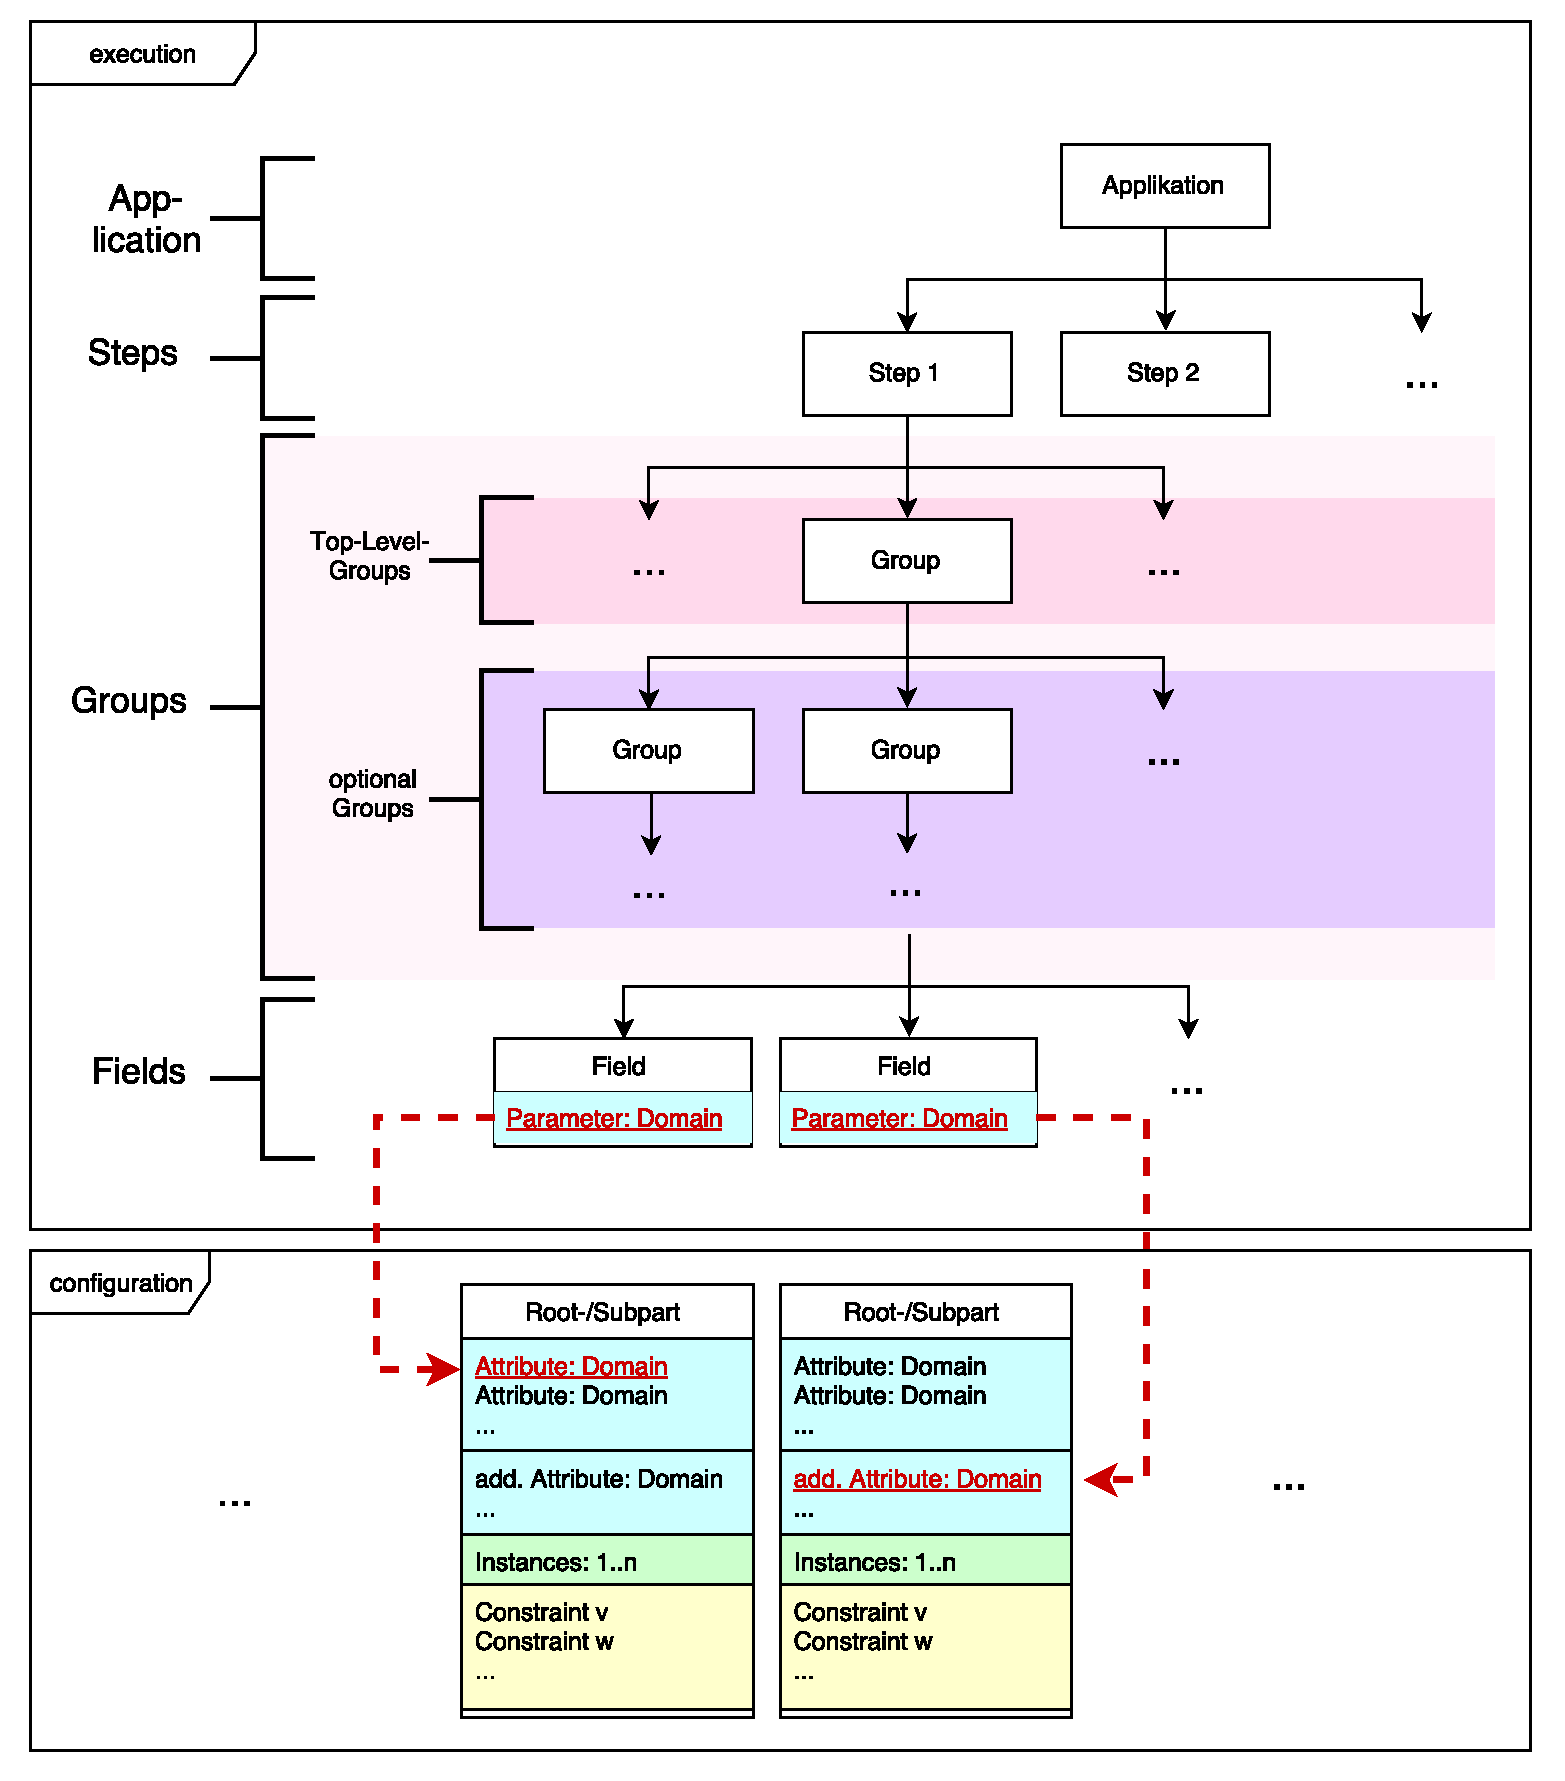
\includegraphics[width=1\linewidth]{Abbildungen/tactonModellExecution.pdf}
	\captionof{figure}[Vollständige Darstellung der generischen Execution-Struktur]{Vollständige Darstellung der generischen Execution-Struktur}
	\label{app:tactonModellExecutionLong}
\end{minipage}
\vspace{1em}

\vspace{1em}
\begin{minipage}{\linewidth}
	\centering
	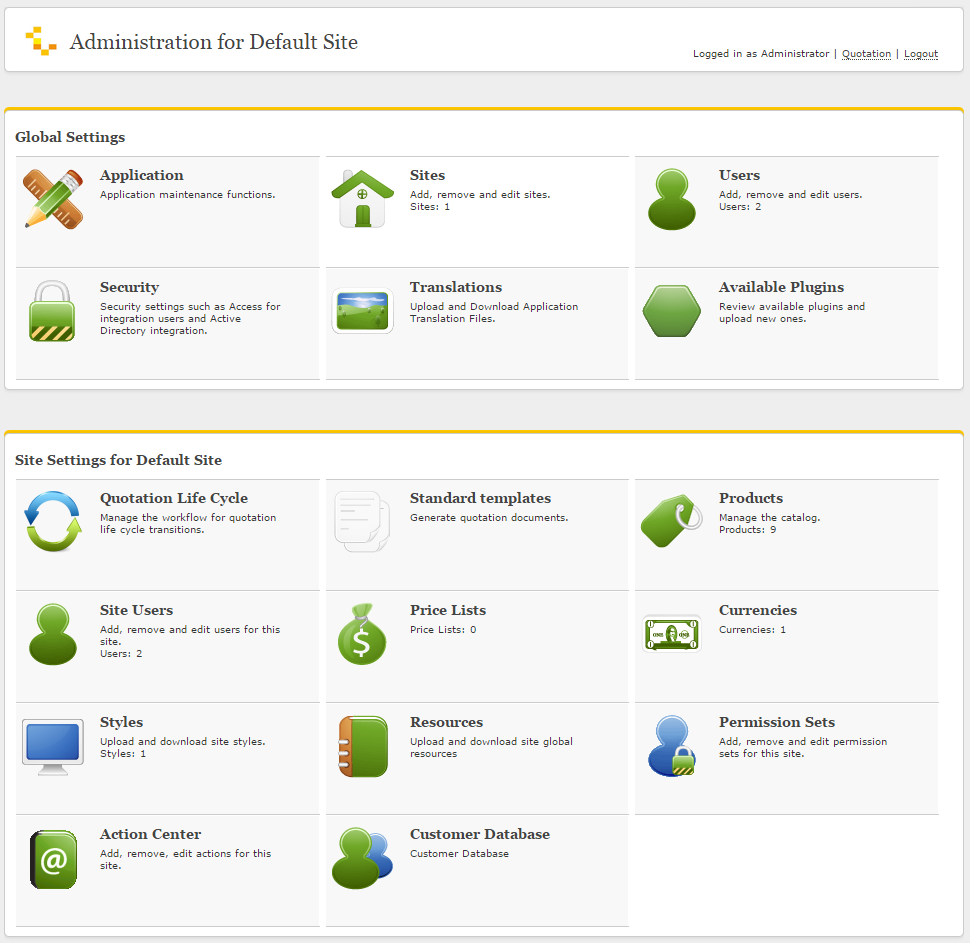
\includegraphics[width=1\linewidth]{Abbildungen/tcsiteAdministration.PNG}
	\captionof{figure}[tcsiteAdministration]{TCsite Administrationsoberfläche}
	\label{app:tcsiteAdministration}
\end{minipage}
\vspace{1em}

\vspace{1em}
\begin{minipage}{\linewidth}
	\centering
	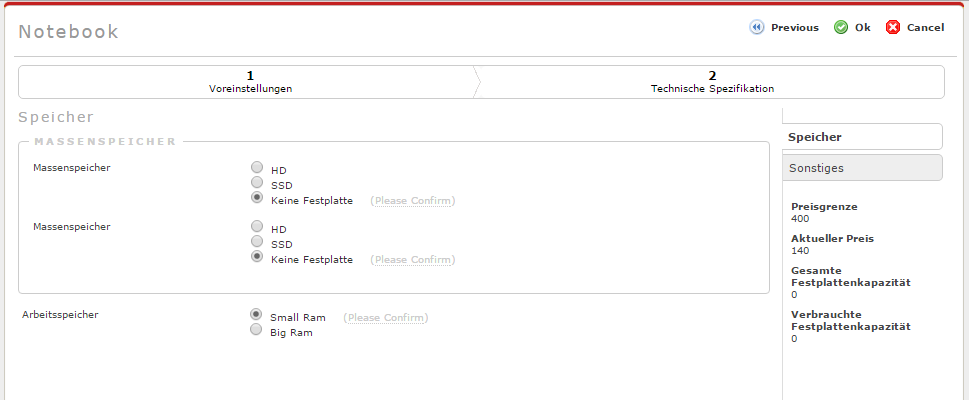
\includegraphics[width=1\linewidth]{Abbildungen/tcSiteConfigurationOptionalGroups.PNG}
	\captionof{figure}[tcSiteConfigurationOptionalGroups]{Darstellung optionaler Groups in TCsite}
	\label{app:tcSiteConfigurationOptionalGroups}
\end{minipage}
\vspace{1em}

\vspace{1em}
\begin{minipage}{\linewidth}
	\centering
	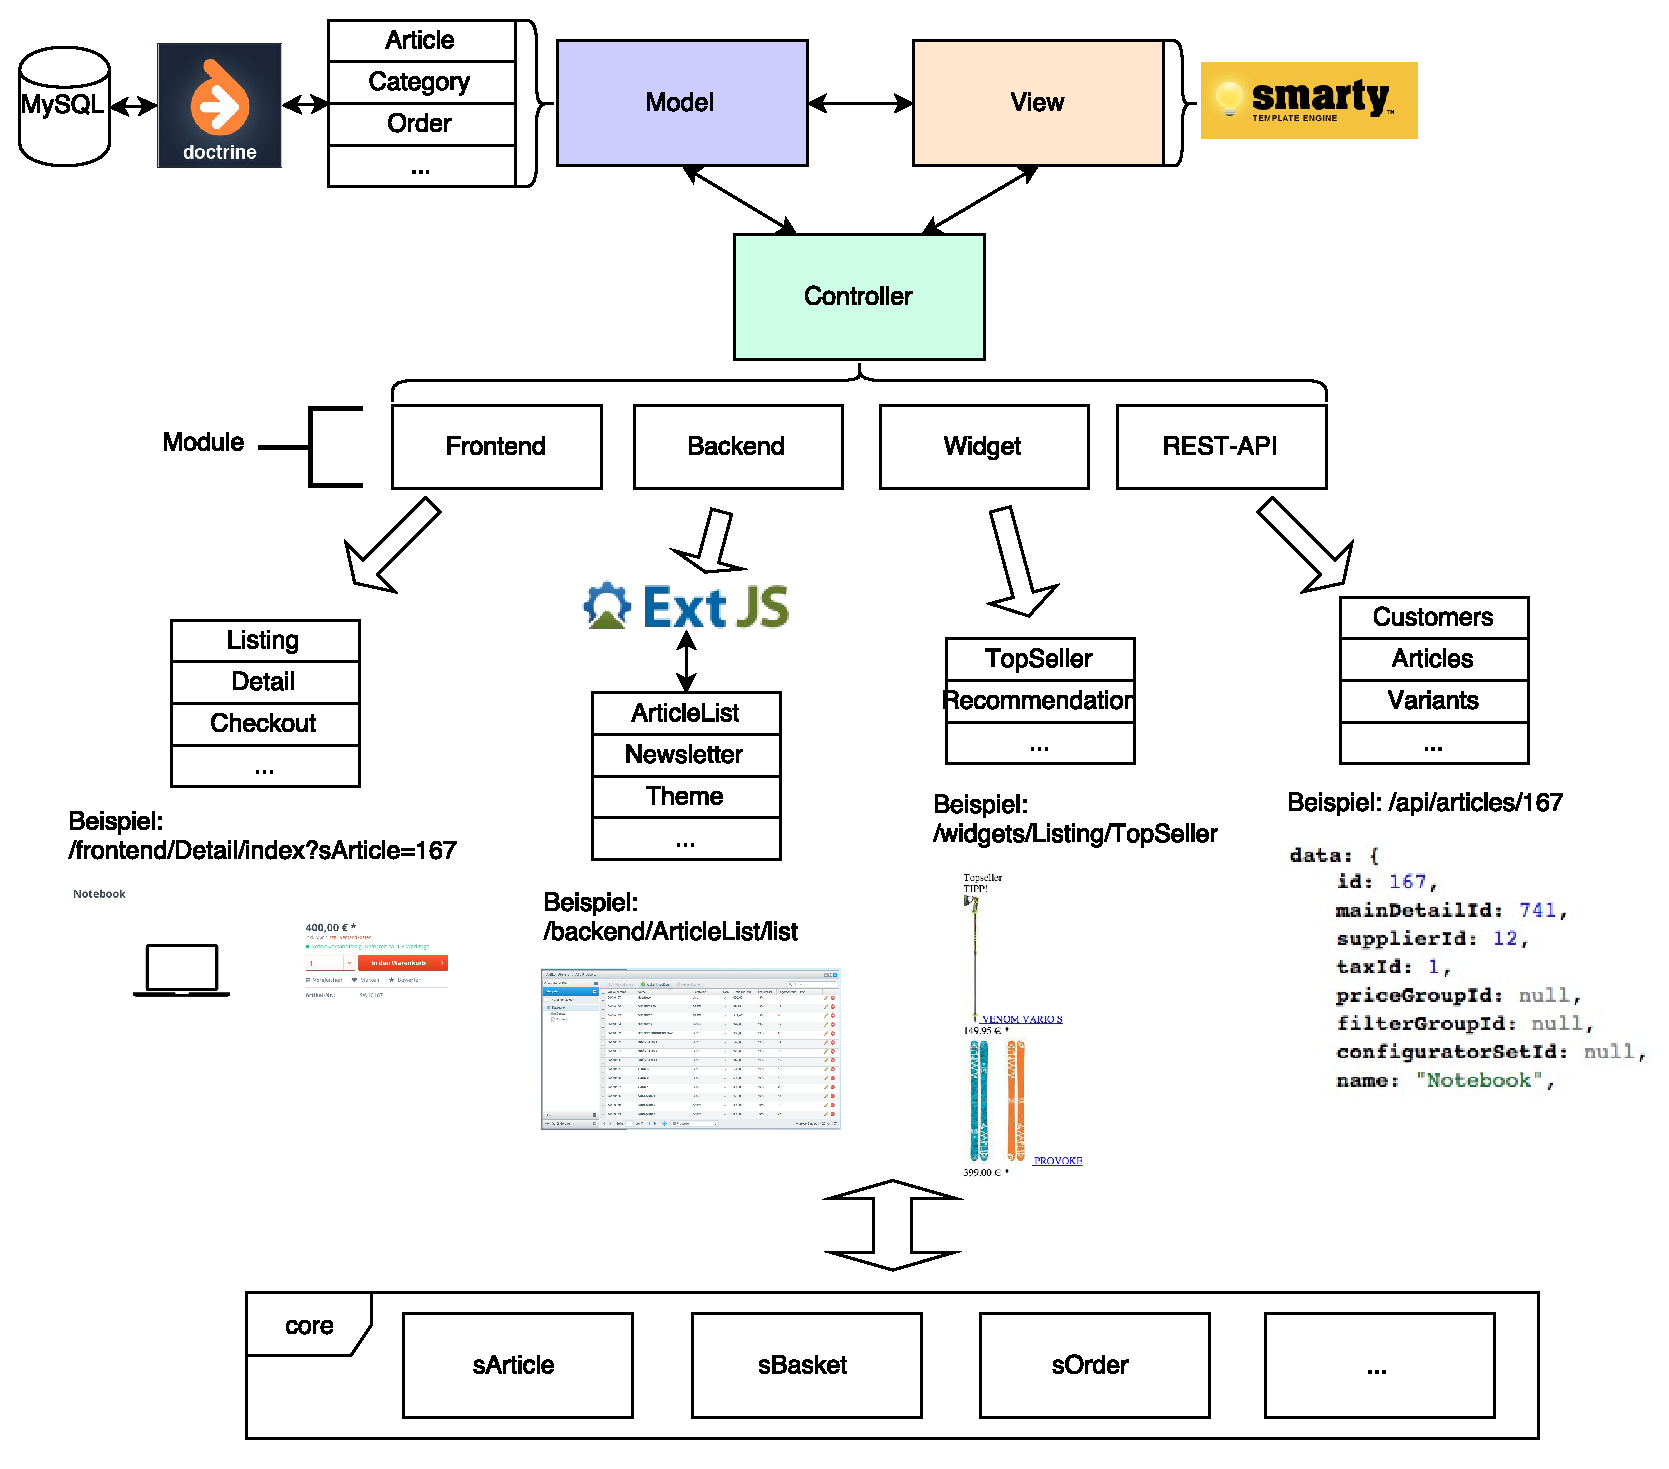
\includegraphics[width=1\linewidth]{Abbildungen/shopwareMVC.pdf}
	\captionof{figure}[vollständige High-Level-Architektur von Shopware]{vollständige Shopware High-Level-Architektur}
	\label{fig:shopwareMVCLong}
\end{minipage}
\vspace{1em}

\vspace{1em}
\begin{minipage}{\linewidth}
	\centering
	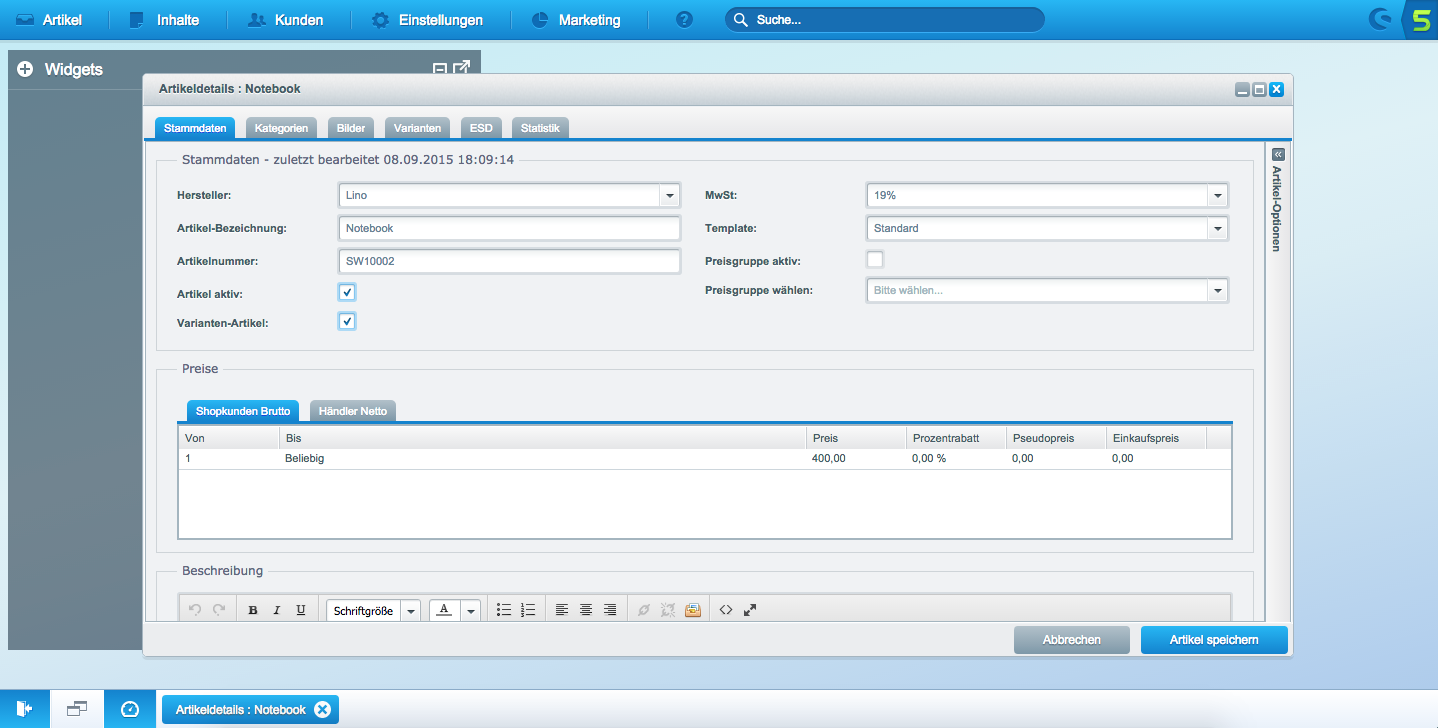
\includegraphics[width=1\linewidth]{Abbildungen/shopwareBackendArtikel.png}
	\captionof{figure}[shopwareBackendArtikel]{Anlegen eines Artikels im Backend}
	\label{app:shopwareBackendArtikel}
\end{minipage}
\vspace{1em}

\vspace{1em}
\begin{minipage}{\linewidth}
	\centering
	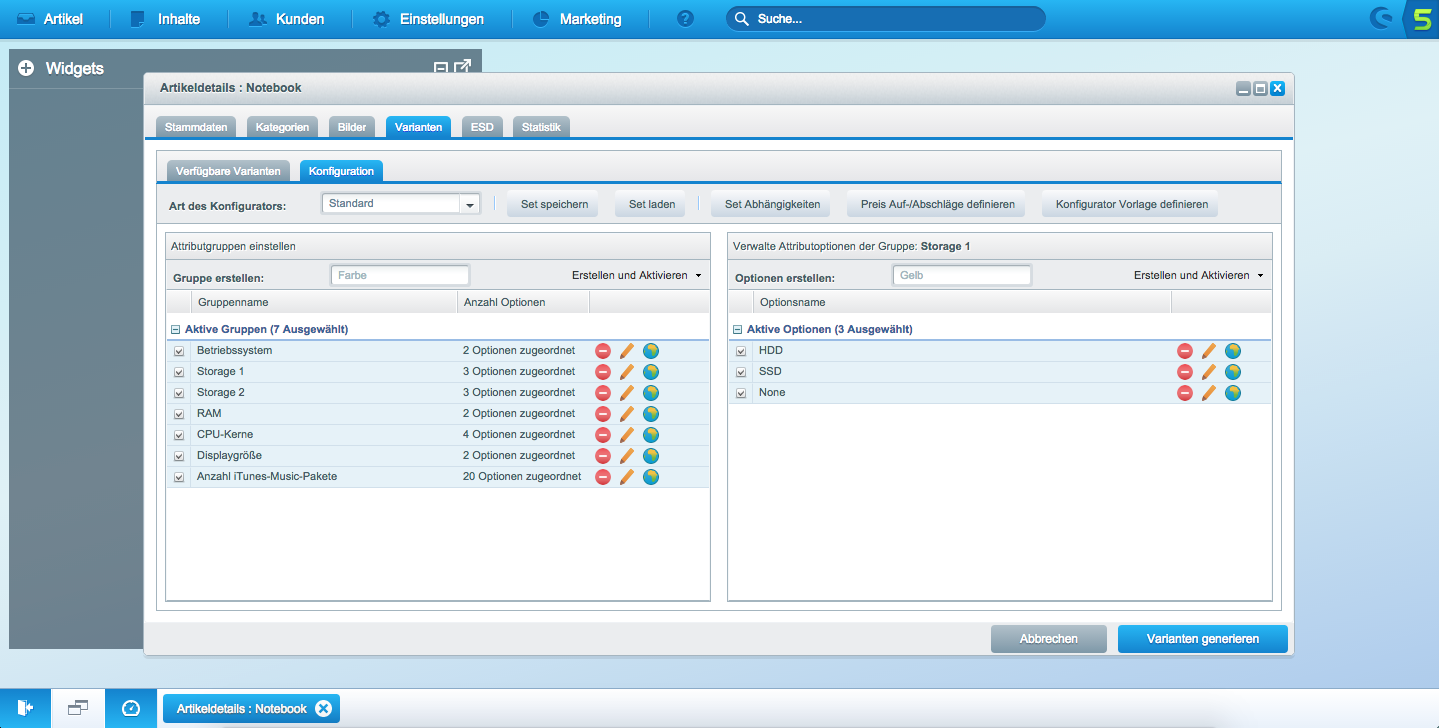
\includegraphics[width=1\linewidth]{Abbildungen/shopwareBackendArtikelVarianten.png}
	\captionof{figure}[shopwareBackendArtikelVarianten]{Generieren der Varianten im Backend}
	\label{app:shopwareBackendArtikelVarianten}
\end{minipage}
\vspace{1em}

\vspace{1em}
\begin{minipage}{\linewidth}
	\centering
	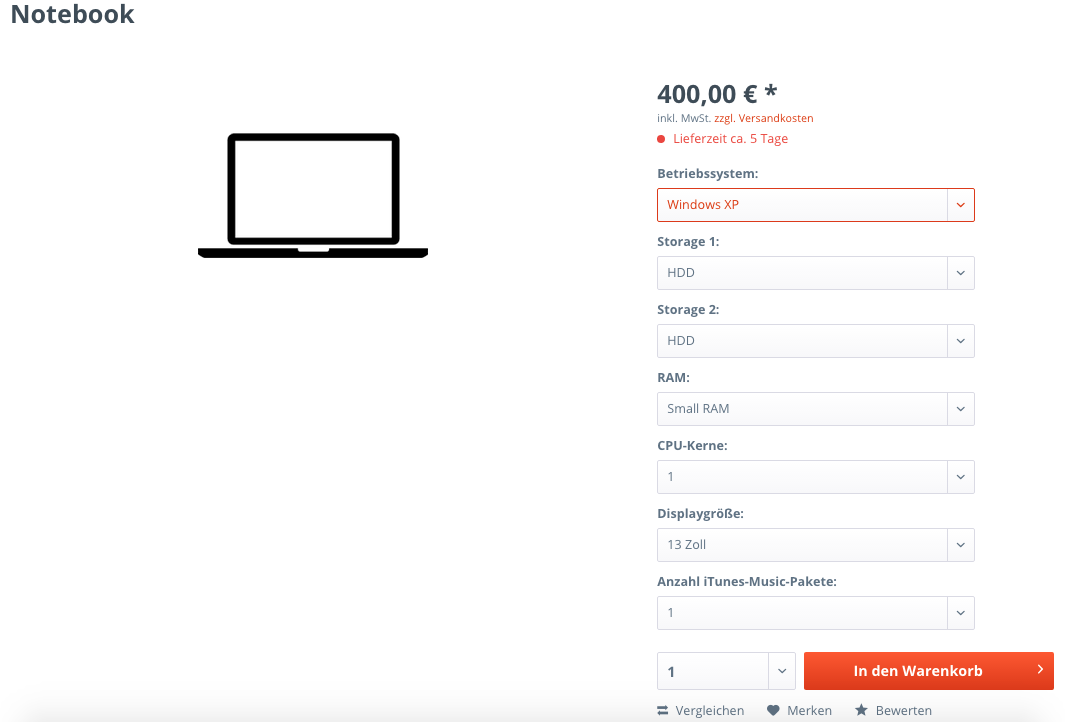
\includegraphics[width=1\linewidth]{Abbildungen/shopwareNotebookDetail.png}
	\captionof{figure}[shopwareNotebookDetail]{Detailansicht eines konfigurierbaren Notebooks in shopware.}
	\label{app:shopwareNotebookDetail}
\end{minipage}
\vspace{1em}

\vspace{1em}
\begin{minipage}{\linewidth}
	\centering
	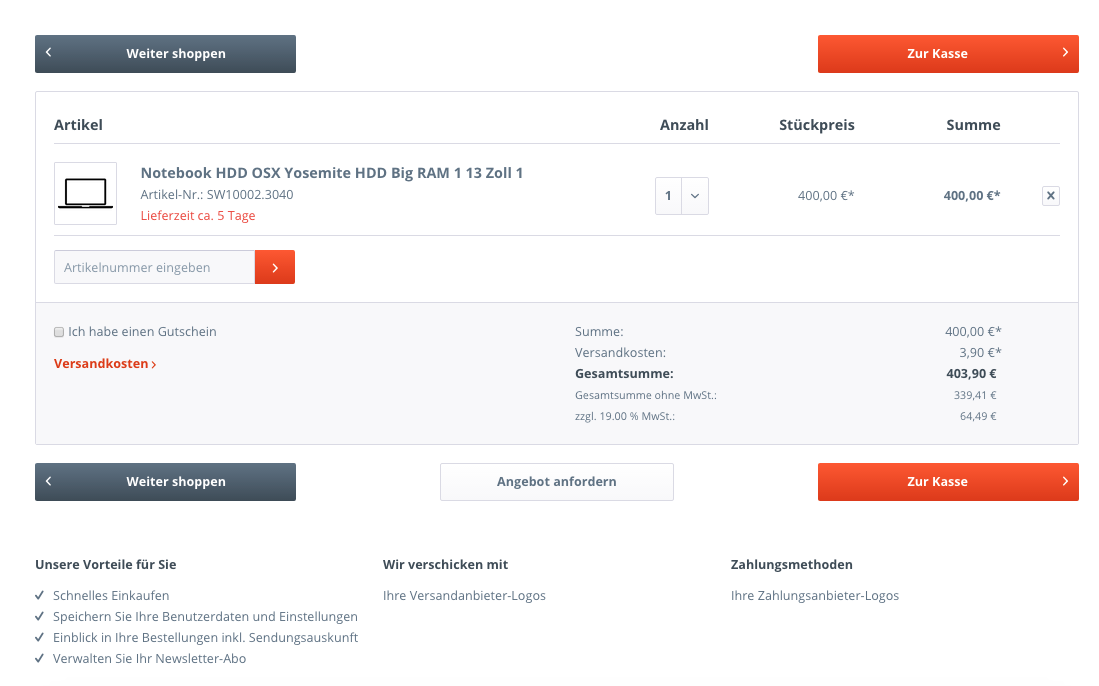
\includegraphics[width=1\linewidth]{Abbildungen/shopwareNotebookWarenkorb.png}
	\captionof{figure}[shopwareNotebookWarenkorb]{Warenkorb mit konfiguriertem Artikel.}
	\label{app:shopwareNotebookWarenkorb}
\end{minipage}
\vspace{1em}

\vspace{1em}
\begin{minipage}{\linewidth}
	\centering
	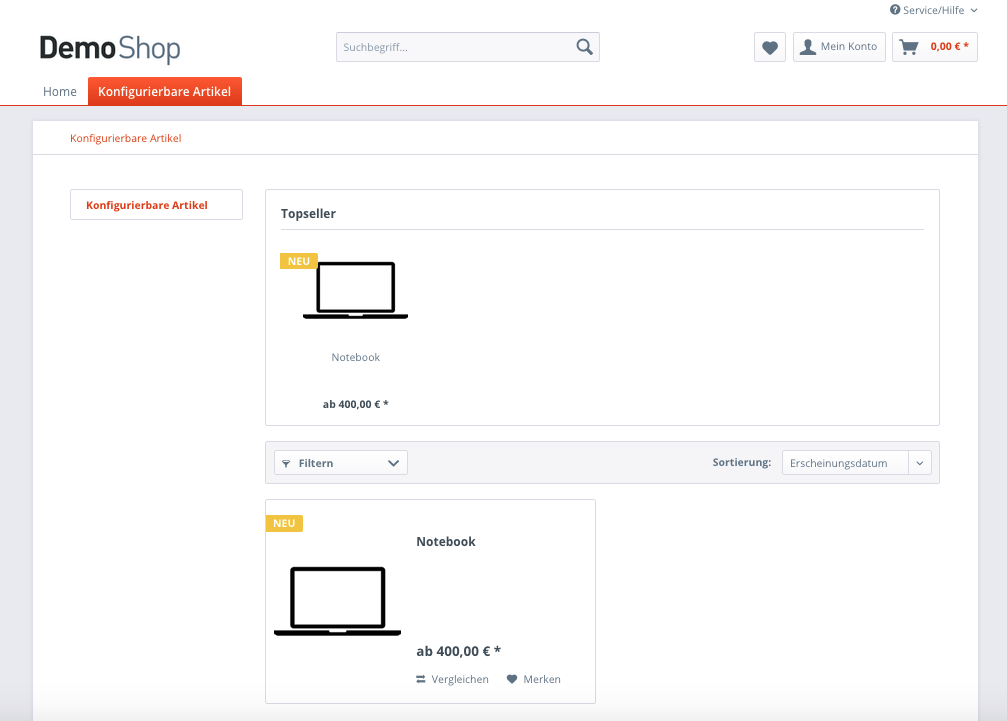
\includegraphics[width=1\linewidth]{Abbildungen/shopwareArtikelListing.png}
	\captionof{figure}[Artikellisting in Shopware]{Artikellisting in Shopware}
	\label{app:shopwareArtikelListing}
\end{minipage}
\vspace{1em}

\vspace{1em}
\begin{minipage}{\linewidth}
	\centering
	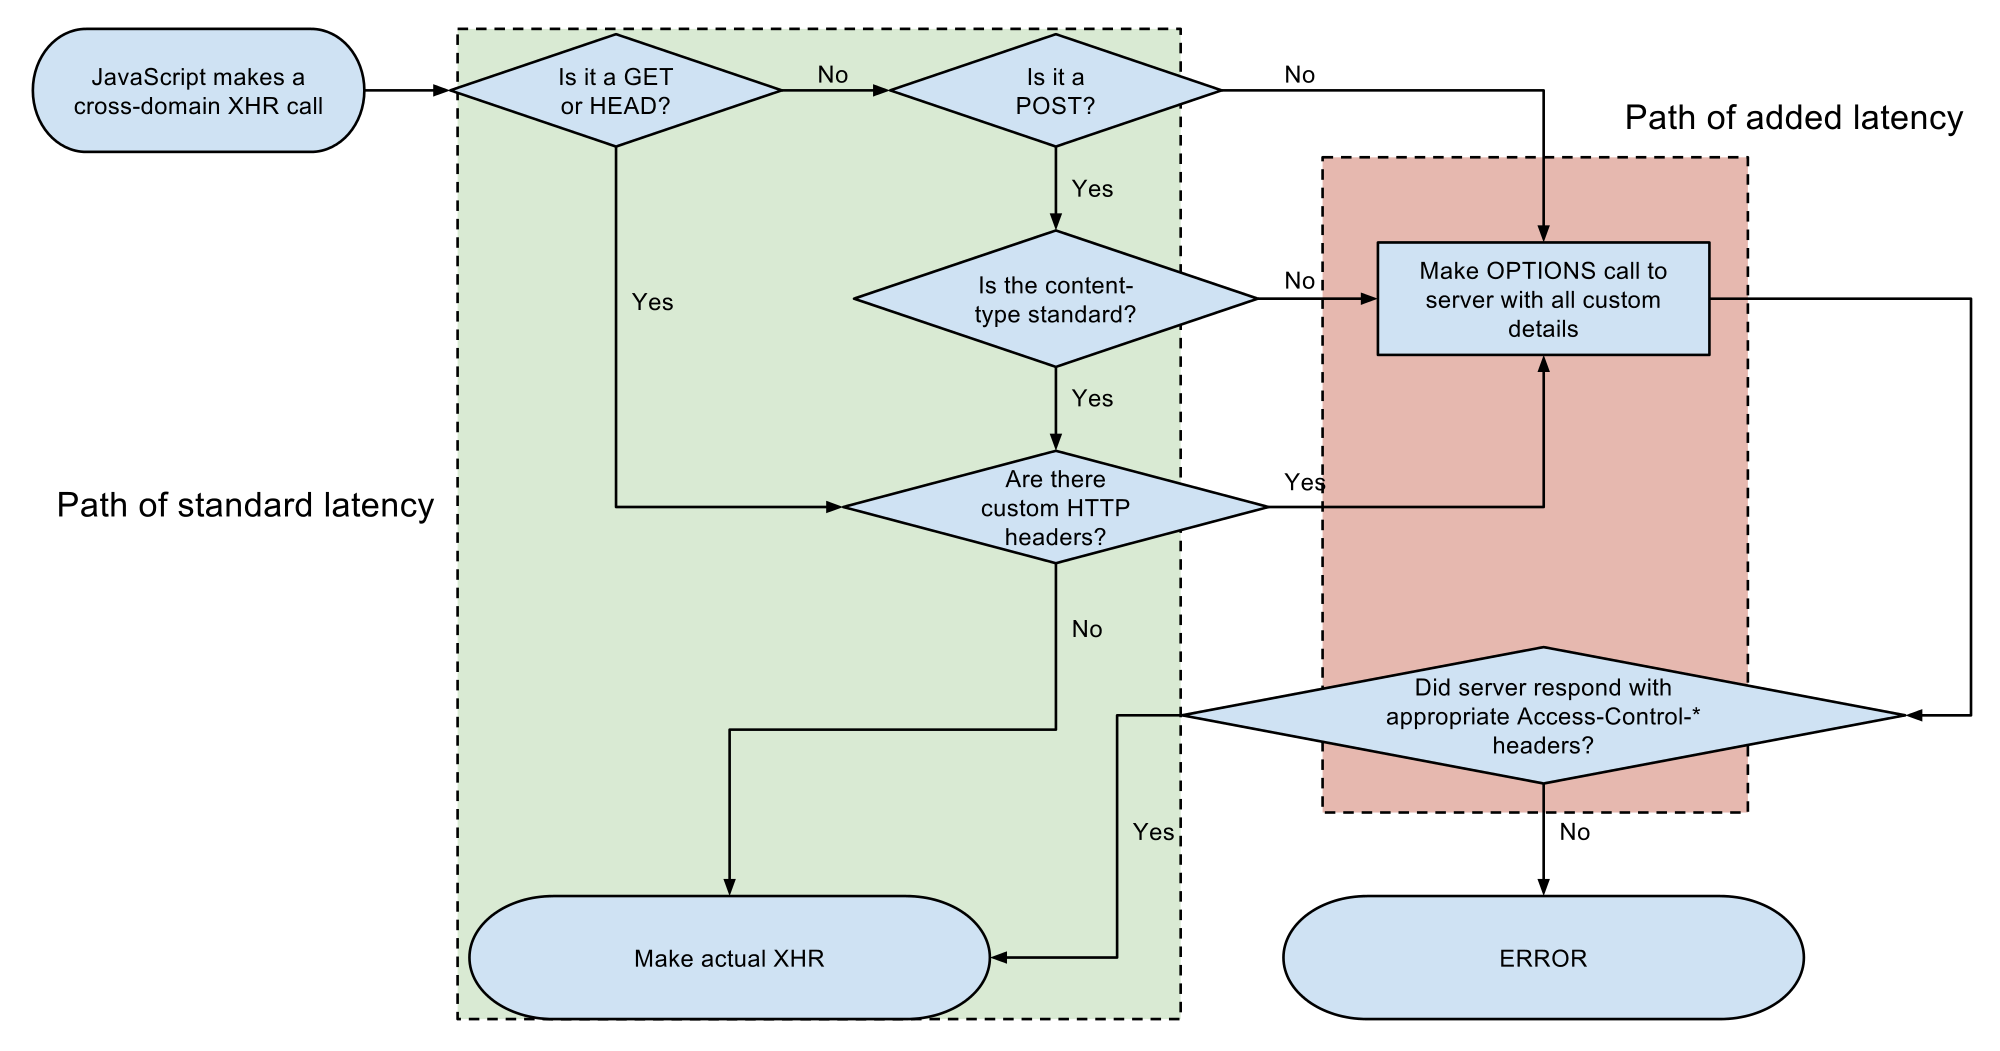
\includegraphics[width=1\linewidth]{Abbildungen/mozillaCORS.png}
	\captionof{figure}[mozillaCORS]{CORS-Flowchart.}
	\label{app:mozillaCORS}
\end{minipage}
\vspace{1em}

\end{appendix}

\chapter*{Selbstständigkeitserklärung}
\vspace{2em}
Ich versichere hiermit an Eides statt, dass ich die vorliegende Bachelorarbeit selbstständig und ohne unzulässige fremde Hilfe erbracht habe. Ich habe keine anderen als die angegebenen Quellen und Hilfsmittel benutzt sowie wörtliche und sinngemäße Zitate kenntlich gemacht. Die Arbeit hat in gleicher oder ähnlicher Form noch keiner Prüfungsbehörde
vorgelegen.

\vspace{4em}
\begin{minipage}{\linewidth}
	\begin{tabular}{p{15em}p{15em}}
		Datum: &  .......................................................\\
		& \centering (Unterschrift)\\
	\end{tabular}
\end{minipage}

\end{document}
